%\documentclass{article}
\documentclass{huawei}

% if you need to pass options to natbib, use, e.g.:
%     \PassOptionsToPackage{numbers, compress}{natbib}
% before loading neurips_2026

% The authors should use one of these tracks.
% Before accepting by the NeurIPS conference, select one of the options below.
% 0. "default" for submission
%\usepackage[preprint]{neurips_2026}
% the "default" option is equal to the "main" option, which is used for the Main Track with double-blind reviewing.
% 1. "main" option is used for the Main Track
%  \usepackage[main]{neurips_2026}
% 2. "position" option is used for the Position Paper Track
%  \usepackage[position]{neurips_2026}
% 3. "eandd" option is used for the Evaluations & Datasets Track
 % \usepackage[eandd]{neurips_2026}
% 4. "creativeai" option is used for the Creative AI Track
%  \usepackage[creativeai]{neurips_2026}
% 5. "sglblindworkshop" option is used for the Workshop with single-blind reviewing
 % \usepackage[sglblindworkshop]{neurips_2026}
% 6. "dblblindworkshop" option is used for the Workshop with double-blind reviewing
%  \usepackage[dblblindworkshop]{neurips_2026}

% After being accepted, the authors should add "final" behind the track to compile a camera-ready version.
% 1. Main Track
 % \usepackage[main, final]{neurips_2026}
% 2. Position Paper Track
%  \usepackage[position, final]{neurips_2026}
% 3. Evaluations & Datasets Track
 % \usepackage[eandd, final]{neurips_2026}
% 4. Creative AI Track
%  \usepackage[creativeai, final]{neurips_2026}
% 5. Workshop with single-blind reviewing
%  \usepackage[sglblindworkshop, final]{neurips_2026}
% 6. Workshop with double-blind reviewing
%  \usepackage[dblblindworkshop, final]{neurips_2026}
% Note. For the workshop paper template, both \title{} and \workshoptitle{} are required, with the former indicating the paper title shown in the title and the latter indicating the workshop title displayed in the footnote.
% For workshops (5., 6.), the authors should add the name of the workshop, "\workshoptitle" command is used to set the workshop title.
% \workshoptitle{WORKSHOP TITLE}

% "preprint" option is used for arXiv or other preprint submissions
 % \usepackage[preprint]{neurips_2026}

% to avoid loading the natbib package, add option nonatbib:
%    \usepackage[nonatbib]{neurips_2026}
\usepackage{amssymb} 
%\usepackage{newtxtext,newtxmath}
%\usepackage{libertinus}
%\usepackage{microtype}
%\usepackage{newtxmath}

\usepackage[T1]{fontenc}
%\usepackage{libertinus}
%\usepackage{XCharter}
\usepackage{newpxtext,newpxmath}
%\usepackage{mathpazo}
%\usepackage{microtype}
\usepackage{microtype}
\usepackage{setspace}
\usepackage{xcolor}

\setstretch{1.15}


%\usepackage{tgpagella}
%\usepackage{newtxmath}

\usepackage[most]{tcolorbox}
\usepackage[table]{xcolor}

\usepackage{xeCJK}
%\setCJKmainfont{Noto Serif CJK SC}


\definecolor{deepblue}{RGB}{37,99,235}
\definecolor{lightblue}{RGB}{239,246,255}



\usepackage[utf8]{inputenc} % allow utf-8 input
\usepackage[T1]{fontenc}    % use 8-bit T1 fonts
\usepackage{hyperref}       % hyperlinks
\usepackage{url}            % simple URL typesetting
\usepackage{booktabs}       % professional-quality tables
\usepackage{amsfonts}       % blackboard math symbols
\usepackage{nicefrac}       % compact symbols for 1/2, etc.
\usepackage{microtype}      % microtypography
\usepackage{fancyhdr}  % 引入自定义页眉页脚的宏包
\usepackage{graphicx}
\usepackage{soul}

\usepackage{multirow}
\usepackage{multicol}
\usepackage{makecell}
\usepackage{arydshln}

\usepackage{enumitem}
\usepackage{xcolor}


\usepackage{graphicx}
\usepackage{fancyhdr}
\usepackage{xcolor}


% \pagestyle{fancy}
% \fancyhf{}
% \setlength{\headheight}{24pt}
% \fancyhead[L]{\textbf{OSU NLP}}
% \fancyhead[R]{Jian Xie et al.}
% \renewcommand{\headrulewidth}{0.8pt}



\begin{document}
% \vspace*{-25mm}

% Note. For the workshop paper template, both \title{} and \workshoptitle{} are required, with the former indicating the paper title shown in the title and the latter indicating the workshop title displayed in the footnote. 
\title{
SearchArt: Training Long-Horizon Search Agent with Scalable Synthetic and Verified Tasks
\vspace{-3mm}
}

% The \author macro works with any number of authors. There are two commands
% used to separate the names and addresses of multiple authors: \And and \AND.
%
% Using \And between authors leaves it to LaTeX to determine where to break the
% lines. Using \AND forces a line break at that point. So, if LaTeX puts 3 of 4
% authors names on the first line, and the last on the second line, try using
% \AND instead of \And before the third author name.


\author{
Huawei Cloud Post-Training Team\footnote{We welcome discussion, collaboration, and contributions to SearchArt: chenchong55@huawei.com, meilang1@huawei.com}
\vspace{-5mm}
% (Full Author List in Section-Contributions)
}



%MiroThinker-1.7 & H1: Towards Heavy-Duty Research Agents via Verification，pdf地址是https://arxiv.org/pdf/2603.15726 
%Marco DeepResearch: Unlocking Efficient Deep Research Agents via Verification-Centric Design，pdf地址是https://arxiv.org/pdf/2603.28376 
%REDSearcher: A Scalable and Cost-Efficient Framework for Long-Horizon Search Agents，pdf地址是https://arxiv.org/pdf/2602.14234 
%LongSeeker: Elastic Context Orchestration for Long-Horizon Search Agents，pdf地址是https://arxiv.org/pdf/2605.05191 
%OpenSeeker-v2: Pushing the Limits of Search Agents with Informative and High-Difficulty Trajectories，pdf地址是https://arxiv.org/pdf/2605.04036 
%QUEST: Training Frontier Deep Research Agents with Fully Synthetic Tasks，pdf地址是https://arxiv.org/pdf/2605.24218




% Expand the above academic content professionally, reasonably, and concisely.
% Make professional, reasonably, and concise revisions to the writing of the above academic content.
% Compress the above academic content professionally, reasonably, and concisely.
% Analyze, summarize, and categorize the aforementioned academic content.




%\begin{myabstract}

%\end{myabstract}

\abstract{
Recent advances in large language models (LLMs) have enabled search agents to autonomously tackle complex tasks across extended search and reasoning horizons.
% \st{multi-step information retrieval and long-horizon reasoning}. 
However, training effective search agents remains challenging due to the lack of scalable and long-horizon tasks, 
% \st{the scarcity of high-quality question-answer (QA) pairs and long-horizon trajectories supervision data, the high cost of human annotation,} 
and the difficulty of evaluating and correcting intermediate reasoning and tool-use behaviors.
% \st{In this technical report,} 
We introduce \textbf{SearchArt}, a scalable framework for training long-horizon search agents through verification-driven task synthesis and a multi-stage post-training pipeline.
SearchArt constructs large-scale datasets for complex \textbf{search}-, \textbf{research}- and \textbf{user}-oriented tasks by synthesizing diverse information-seeking QA pairs and corresponding search trajectories from web documents and automatically generated evidence graphs.
To ensure the reliability of the synthesized data, we design a verification pipeline that jointly evaluates QA consistency, trajectory quality, and the relevance of retrieved evidence. The verified trajectories are subsequently used in a multi-stage training process comprising supervised fine-tuning and reinforcement learning-based policy optimization.
Search agents trained with SearchArt exhibit adaptive search planning, iterative evidence aggregation, and complex reasoning over extended interaction horizons. 
Experimental results demonstrate that, with only (Qwen3.5-) 27B parameters, SearchArt scores \textbf{74.39 on BrowseComp-ZH}, \textbf{70.06 on BrowseComp}, and \textbf{52.55 on Deepresearch-bench}, matching or surpassing frontier closed-source agents on both deepsearch and deepresearch benchmarks.
%Experimental results demonstrate that, with only 27B parameters, SearchArt matches or surpasses frontier closed-source agents on both deep search and deep research benchmarks.
% \st{Experiments on open-domain deep-research benchmarks using the Qwen3.5 model series show that our approach substantially improves task-completion accuracy relative to existing search agents of comparable scale. These results demonstrate that verification-driven synthetic task generation, combined with trajectory-level post-training, provides a practical and scalable pathway toward building more capable and reliable deep-research agents.}
}






\maketitle
\vspace{-8mm}

\begin{figure}[htbp]
    \centering
    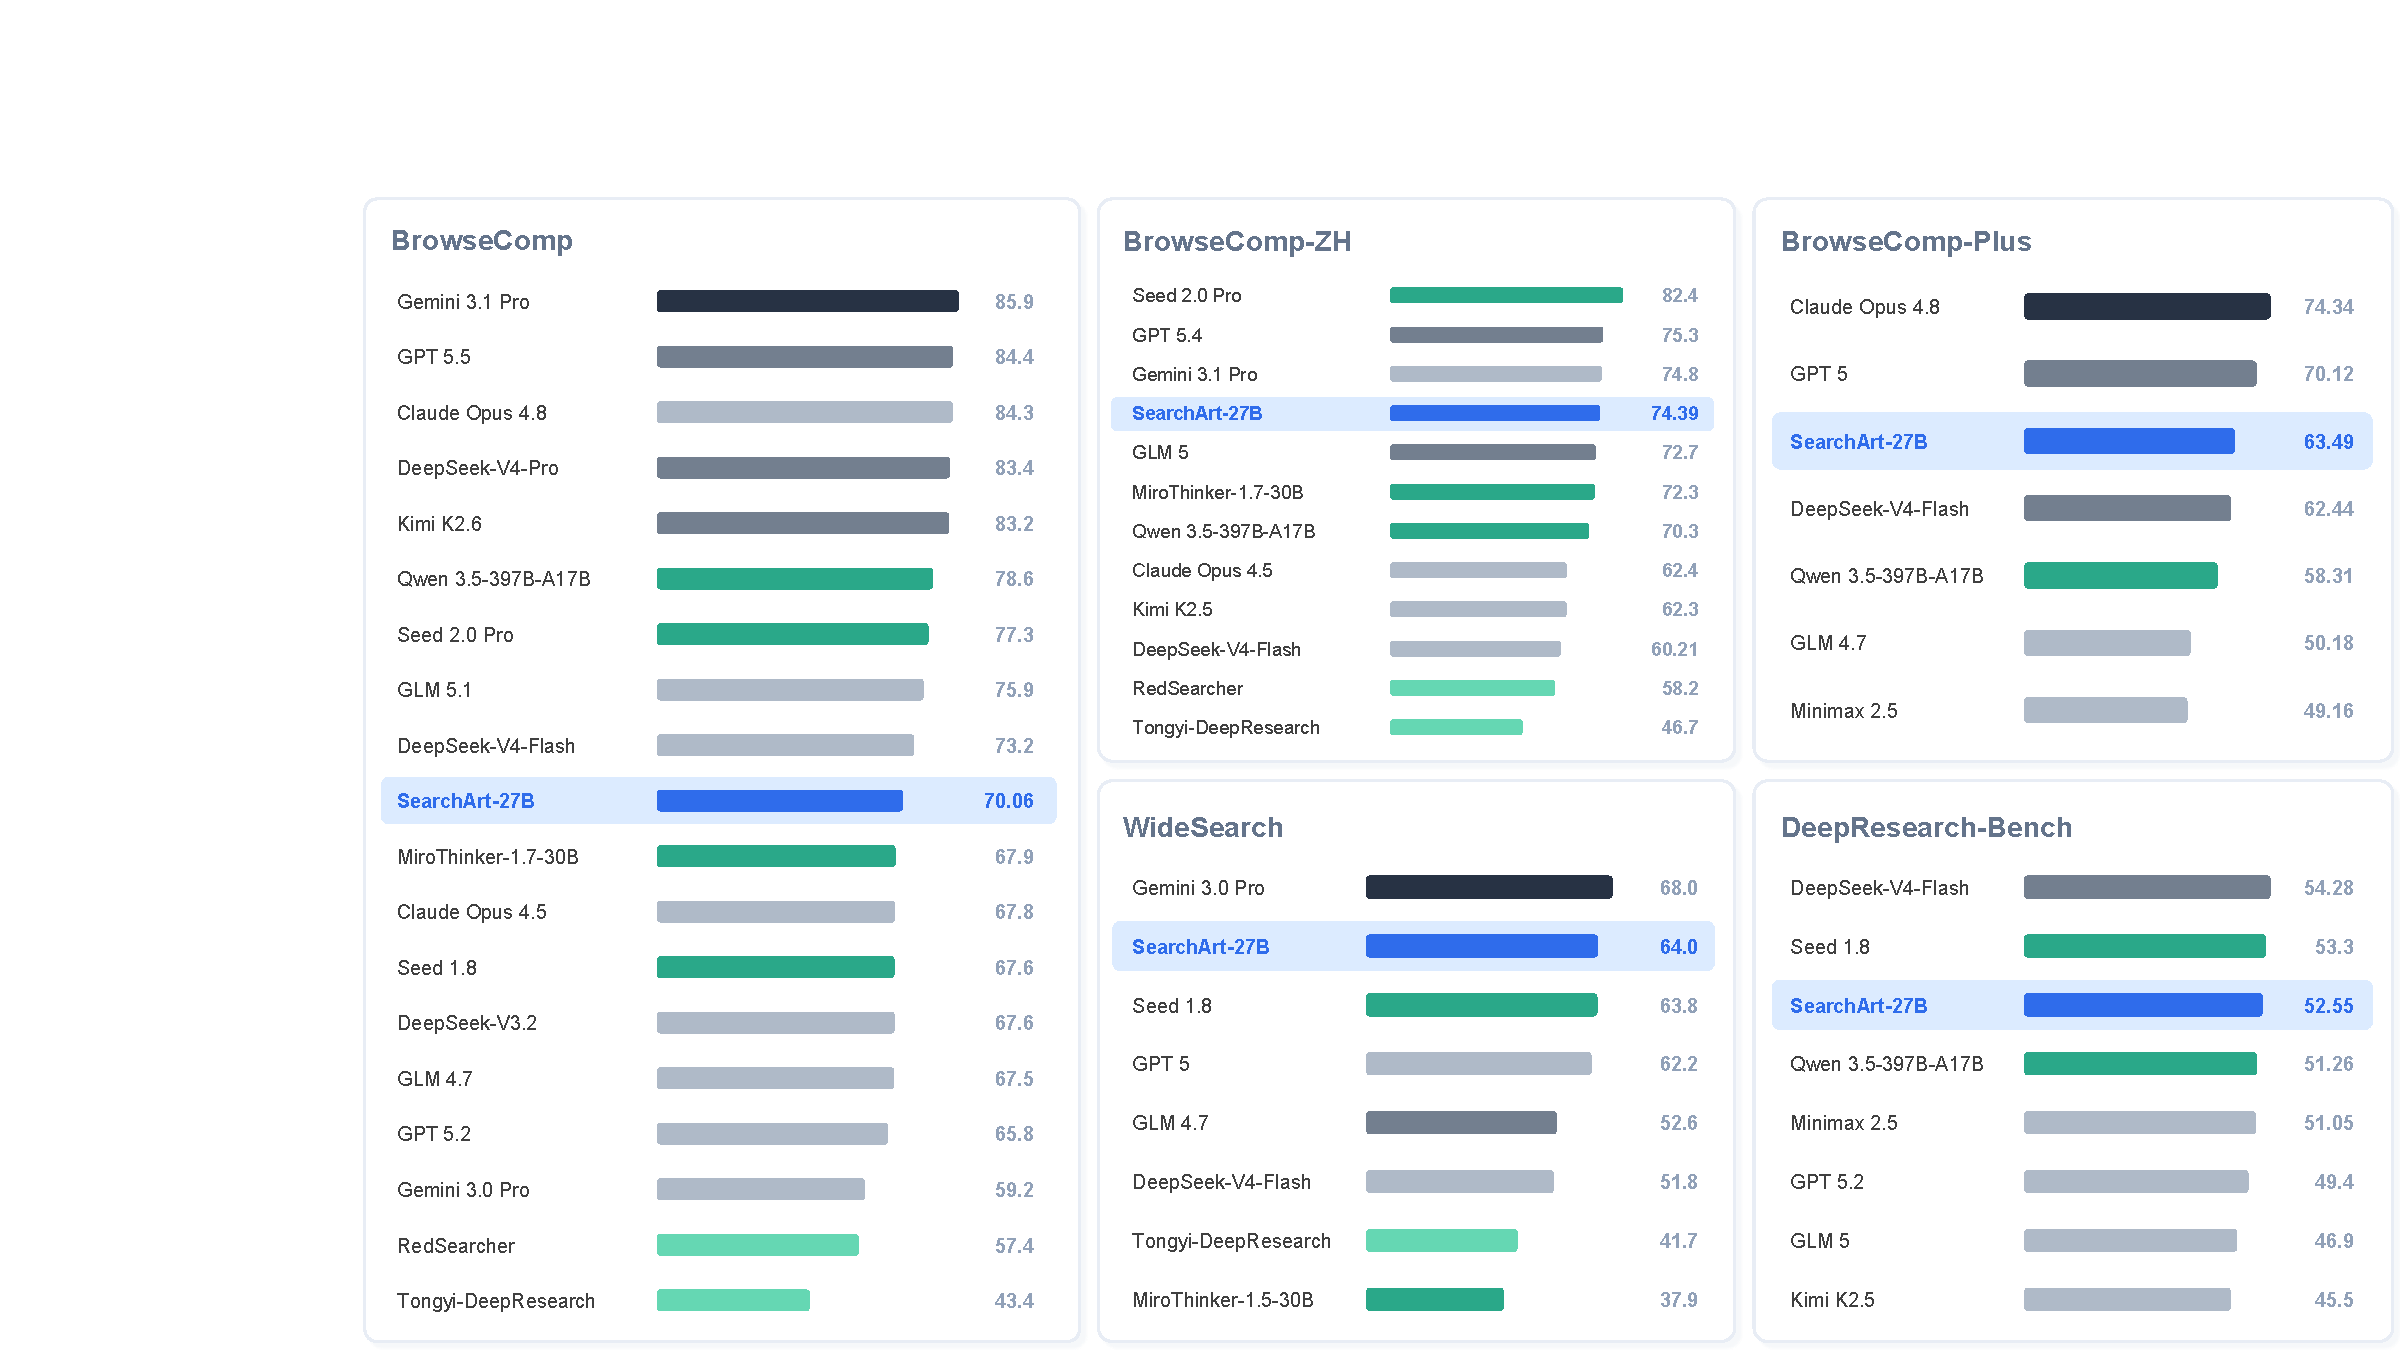
\includegraphics[width=0.96\linewidth]{img/browsecomp_leaderboard_overview_v2.pdf}
    \caption{Comprehensive comparison across five benchmarks that evaluate different capabilities.}
    \label{fig:browsecomp_leaderboard_overview}
\end{figure}

\tableofcontents
\newpage


\section{Introduction}
%大语言模型（LLMs）正日益具备作为自主智能体（autonomous agents）进行搜索、检索与信息综合的能力，并能够在多轮交互过程中完成复杂任务。与仅在固定上下文中进行推理的传统问答系统不同，长程搜索智能体需要动态规划检索行为、持续跟踪不断演化的证据状态，并在长时间推理轨迹中整合来自异构信息源的数据。这些能力对于文献分析、对比研究、科学发现以及战略决策等复杂研究型任务至关重要。
Large language models (LLMs) \cite{naveed2025comprehensive, zhao2023survey, achiam2023gpt, qwenbai2023qwen, liu2024deepseek, guo2025deepseek, xu2026deepseek, yin2024survey} are increasingly capable of acting as autonomous agents for information retrieval and synthesis, enabling them to solve complex tasks through multi-turn interactions.
Unlike conventional question-answering (QA) systems \cite{lewis2020retrieval, gao2023retrieval, mei2025survey, liu2025llm4ranking, gong2026cardrewriter, niu2025distributionally, mei2025dense, niu2025addressing, mei2023improving}, that operate over a fixed context, long-horizon search agents \cite{team2026mirothinker, chu2026redsearcher, deng2026fort, du2026openseeker, zhu2026marco, hu2025step} must dynamically formulate and revise retrieval strategies, maintain evolving representations of the available evidence, and integrate information from heterogeneous sources throughout extended reasoning processes. These capabilities are critical for research-intensive tasks, including literature analysis, comparative studies, scientific discovery, and strategic decision-making.


%尽管智能体推理（agentic reasoning）近年来取得了快速进展，但如何训练高效的搜索智能体仍然是一个充满挑战的核心问题。随着基模型的增强，大多数方法缺少高质量的问答对，面临人工注释的高成本，以及评估和纠正中间推理和工具使用行为的困难，导致了这些方案本质上难以扩展，因为长程研究任务往往需要多样化的检索路径、细致复杂的推理链条以及可靠的证据归因。此外，收集得到的轨迹质量差异较大，长程推理轨迹监督信号较为稀疏，解决问题的范式较为单一，噪声监督很容易导致模型学习到低效的搜索行为、幻觉式推理，或过早生成答案。
Although agentic reasoning \cite{singh2025agentic, wu2025agentic, wu2025agentic1} has advanced rapidly in recent years, training effective search agents \cite{team2026mirothinker, chu2026redsearcher, jin2025search, song2025r1, yu2026m, mei2025ai, xia2026search, gong2024cosearchagent, chen2026unitymas, yang2026tournament, zhang2026oases, chen2025mao, chen2026beyond, chen2026jade, chen2026improving} remains a fundamental challenge. Despite the growing capabilities of LLMs, existing approaches continue to be limited by the scarcity of high-quality QA data, the substantial cost of human annotation, and the difficulty of evaluating and correcting intermediate reasoning and tool-use behaviors.
These limitations hinder scalability, particularly for long-horizon research tasks that require diverse retrieval strategies, complex multi-step reasoning, and reliable attribution of supporting evidence.
Moreover, collected reasoning trajectories often vary considerably in quality, while supervisory signals for long-horizon reasoning remain sparse and the available solution paradigms relatively homogeneous. Consequently, noisy or insufficient supervision may lead models to adopt inefficient search strategies, generate unsupported reasoning (i.e., hallucination), or produce answers prematurely before adequate evidence has been gathered.


%越来越多的近期研究表明，合成任务生成与自动化验证可能为替代人工标注提供可扩展的解决方案。然而，当前方法仍然存在若干局限性。首先，许多合成数据流程更关注最终答案的正确性，而忽略了中间搜索决策与证据迁移过程的质量。其次，较弱的过滤机制往往会保留浅层或冗余的轨迹，无法有效训练智能体的探索能力。第三，现有训练语料通常对需要长期信息积累与自适应检索规划的高难度长程任务覆盖不足。
A growing body of recent research \cite{team2026mirothinker, chu2026redsearcher, deng2026fort, du2026openseeker, zhu2026marco, hu2025step} indicates that synthetic task generation and automated verification can serve as scalable alternatives to human annotation. 
Nevertheless, existing approaches continue to face several important limitations. 
First, many synthetic data pipelines emphasize final-answer correctness while paying insufficient attention to the quality of intermediate search decisions and transitions between pieces of evidence.
Second, weak filtering procedures often retain shallow, repetitive, or redundant trajectories, thereby providing limited supervision for learning effective exploration strategies.
Third, existing training corpora frequently underrepresent challenging, long-horizon tasks that require sustained information integration, iterative reasoning, and adaptive retrieval planning.




% 在这份技术报告中，我们提出了一种可扩展的框架，通过“验证驱动的合成任务生成（verification-driven synthetic task generation）”以及多阶段后训练流程来训练长程搜索智能体。我们的方法通过从网页文档和自动生成的证据图（evidence graphs）中合成多样化的多跳信息检索问答对及其轨迹，构建了大规模复杂搜索与研究导向任务的数据集。为了保证合成问答对与轨迹的质量，我们设计了一套验证流程，对问答一致性、轨迹质量以及检索证据相关性进行联合评估。经过验证的轨迹随后被用于监督微调（supervised fine-tuning）和基于强化学习的策略优化。在训练过程中，智能体学习如何在长程任务中协调检索与推理行为、选择性扩展证据分支，并根据任务复杂度自适应地分配搜索预算。与主要优化最终答案监督的现有方法相比，我们的框架显式建模了中间智能体行为的质量，从而能够学习更加稳定且高效的搜索策略。
In this technical report, we introduce \textbf{SearchArt}, a scalable framework for training long-horizon search agents through verification-driven synthetic task generation and a multi-stage post-training pipeline.
SearchArt constructs large-scale datasets for complex \textbf{search}-, \textbf{research}- and \textbf{user}-oriented tasks by synthesizing diverse information-seeking QA pairs, together with their corresponding search trajectories, from web documents and automatically generated evidence graphs.
To ensure the quality of the synthesized data, we develop a verification pipeline that jointly evaluates QA consistency, trajectory reliability, and the relevance of retrieved evidence. The verified trajectories are subsequently utilized for supervised fine-tuning and reinforcement learning–based policy optimization.
Through training process, the agent learns to coordinate retrieval and reasoning over long-horizon tasks, selectively expand evidence branches, and adaptively allocate search budgets according to task complexity. 
In contrast to prior approaches that primarily optimize for final-answer supervision, SearchArt explicitly models and optimizes the quality of intermediate search and reasoning behaviors. This design yields more stable, efficient, and reliable search policies for complex information-seeking tasks.




%基于该框架，我们进一步提出了 Training Long-Horizon Search Agents with Scalable Synthetic and Verified Tasks，这是一套利用自动生成监督信号构建深度研究智能体的可扩展训练方案。我们在多个开放域研究与多跳推理基准上对该方法进行了评估。实验结果表明，与现有搜索智能体训练方法相比，我们的方法在任务成功率、证据质量、检索效率以及长上下文推理鲁棒性等方面均取得了持续提升。特别是在需要大规模证据聚合与深层推理的高难度任务上，我们的方法表现出了显著优势。
Building on this framework and Qwen3.5-27B model, we evaluate our approach on a diverse set of open-domain deep-research and multi-hop reasoning benchmarks. 
Experimental results show that SearchArt, despite having only 27B parameters, achieves strong performance across multiple benchmarks, scoring \textbf{74.39 on BrowseComp-ZH}, \textbf{70.06 on BrowseComp}, \textbf{63.49 on BrowseComp-Plus}, \textbf{64.0 on WideSearch}, and \textbf{52.55 on DeepResearch-Bench}.
These findings demonstrate that SearchArt matches or even surpasses frontier closed-source agents on both deep search and deep research tasks, and significantly improves task-completion accuracy relative to existing search agents of comparable scale.
Overall, our work highlights the importance of scalable synthetic supervision and verification-centric training in developing the next generation of deep-research agents. We believe these findings provide a practical foundation for building more capable, efficient, and trustworthy search systems that can operate autonomously over complex information environments.








\section{Scalable Long-Horizon Task Synthesis \& Verification}
%We design a QA synthesis framework with two complementary pipelines: a Corpus-based Pipeline for efficient large-scale generation from structured knowledge graphs, and a Web-Augmented Multi-hop Pipeline (WebHop) that combines web knowledge expansion with explicit difficulty control. The two pipelines jointly provide breadth and depth: the Corpus-based Pipeline produces high-volume QA pairs with diverse question structures and reasoning patterns over curated corpora to build foundational reasoning capability, while WebHop generates fewer but precisely calibrated questions with verified multi-hop structure and open-web grounding. In training, Corpus-based output dominates early stages, and WebHop output is progressively introduced to push the model toward harder and more realistic challenges.



%In this section, we apply explicit verification to QA data synthesis to ensure the quality and answer uniqueness while keeping their difficulties. High-quality QA data is essential for both trajectory synthesis and optimization. A common bottleneck in existing approaches is answer non-uniqueness: to increase question difficulty, most methods obfuscate entity information in multi-hop questions [Team et al., 2025a, Xu et al., 2026b], which inevitably introduces ambiguity and may result in low-quality questions with multiple valid answers. When such data is used as ground truth, the training becomes biased and unstable. We address this problem through two complementary synthesis pipelines: graph-based and agent-based, each incorporating explicit verification to guarantee answer quality.


% In this section, we present a scalable framework for synthesizing long-horizon tasks for the training and evaluation of search agents. The framework is designed to jointly address three objectives: (1) generating realistic information-seeking tasks grounded in open-world knowledge; (2) constructing long-horizon reasoning and retrieval trajectories with controllable complexity; and (3) maintaining answer faithfulness and reliable verification throughout the synthesis process. To this end, we develop three complementary QA synthesis pipelines:
% (1) DeepSearch-oriented pipeline emphasizes scalable generation of retrieval-intensive questions with progressively increasing complexity.
% (2) DeepResearch-oriented pipeline targets research-style tasks that require extended exploration, multi-source evidence aggregation, and long-context reasoning.
% (3) Real-world User Experience–oriented pipeline collects and synthesizes difficult questions that preserve natural user intent, practical decision needs, and realistic interaction patterns, while still requiring nontrivial search depth and breadth.

%\textcolor{red}{
In this section, we present a scalable framework for synthesizing long-horizon tasks for training and evaluating search agents. The framework addresses three objectives: generating realistic information-seeking tasks grounded in open-world knowledge, constructing reasoning and retrieval trajectories with controllable complexity, and ensuring answer faithfulness and reliable verification throughout synthesis. To this end, we develop three complementary QA synthesis pipelines: (1) a DeepSearch-oriented pipeline for scalable generation of retrieval-intensive questions with increasing complexity; (2) a DeepResearch-oriented pipeline for research-style tasks requiring extended exploration, multi-source evidence aggregation, and long-context reasoning; and (3) a Real-world User Experience–oriented pipeline for difficult questions that preserve natural user intent, practical decision needs, and realistic interaction patterns while requiring substantial search depth and breadth.%}


% \subsection{DeepSearch QA Synthesis}
% Our DeepSearch QA synthesis framework is designed to construct challenging, evidence-grounded QA tasks that require sustained web exploration and multi-step reasoning, rather than reliance on parametric knowledge or superficial retrieval. The pipeline follows a progressive synthesis process that transforms carefully selected seed entities into executable long-horizon search tasks. 
% It first initializes seeds that balance knowledge novelty, structural connectivity, and domain coverage, and then expands them into a large-scale evidence-rich knowledge graph through iterative web-enhanced agentic exploration. From this graph, structurally complex and evidence-dispersed subgraphs are sampled and ranked according to their expected reasoning and retrieval difficulty. 
% Finally, the retained knowledge regions are converted into QA instances through a complexity-scaling generation procedure that incrementally introduces longer reasoning chains, distributed evidence dependencies, and hard search trajectories. Together, these stages enable the systematic generation of diverse and controllably difficult DeepSearch QA data, providing a more faithful evaluation of an agent’s ability to acquire, integrate, and reason over open-world information.
% We give the overview and statistics of the DeepSearch QA synthesis in Figure \ref{fig:deepsearch_qa_synthesis_framework} and \ref{fig:synthetic_task_qa_trajectory_distribution_bright}.

\subsection{DeepSearch QA Synthesis}
%\textcolor{red}{
We propose a shortcut-resistant and evidence-dispersed synthesis framework for constructing challenging long-horizon DeepSearch QA tasks. The framework is designed to substantially reduce reliance on parametric knowledge, surface-level retrieval cues, or isolated evidence snippets, while encouraging sustained web exploration, dispersed evidence aggregation, and compositional reasoning. As illustrated in Figures~\redref{fig:deepsearch_qa_synthesis_framework} 
and~\redref{fig:synthetic_task_qa_trajectory_distribution_bright}, the pipeline follows a progressive synthesis process that transforms selected seed entities into executable long-horizon search tasks. It first initializes seeds that balance knowledge novelty, structural connectivity and domain coverage, and then expands them into a large-scale evidence-rich knowledge graph through iterative web-enhanced agentic exploration. Structurally complex subgraphs with dispersed evidence are then sampled and ranked by their estimated reasoning and retrieval difficulty. Finally, these knowledge regions are converted into QA instances through a complexity-scaling process that increases reasoning-chain length, evidence dispersion, and search-trajectory difficulty. This process yields diverse and controllably difficult DeepSearch QA data for faithfully evaluating agent capabilities in open-world information acquisition, evidence integration, and multi-step reasoning.%}
We give QA examples in Appendix \redref{appendix:DeepSearch QA}.


\begin{figure}[!t]%[htbp]
    \centering
    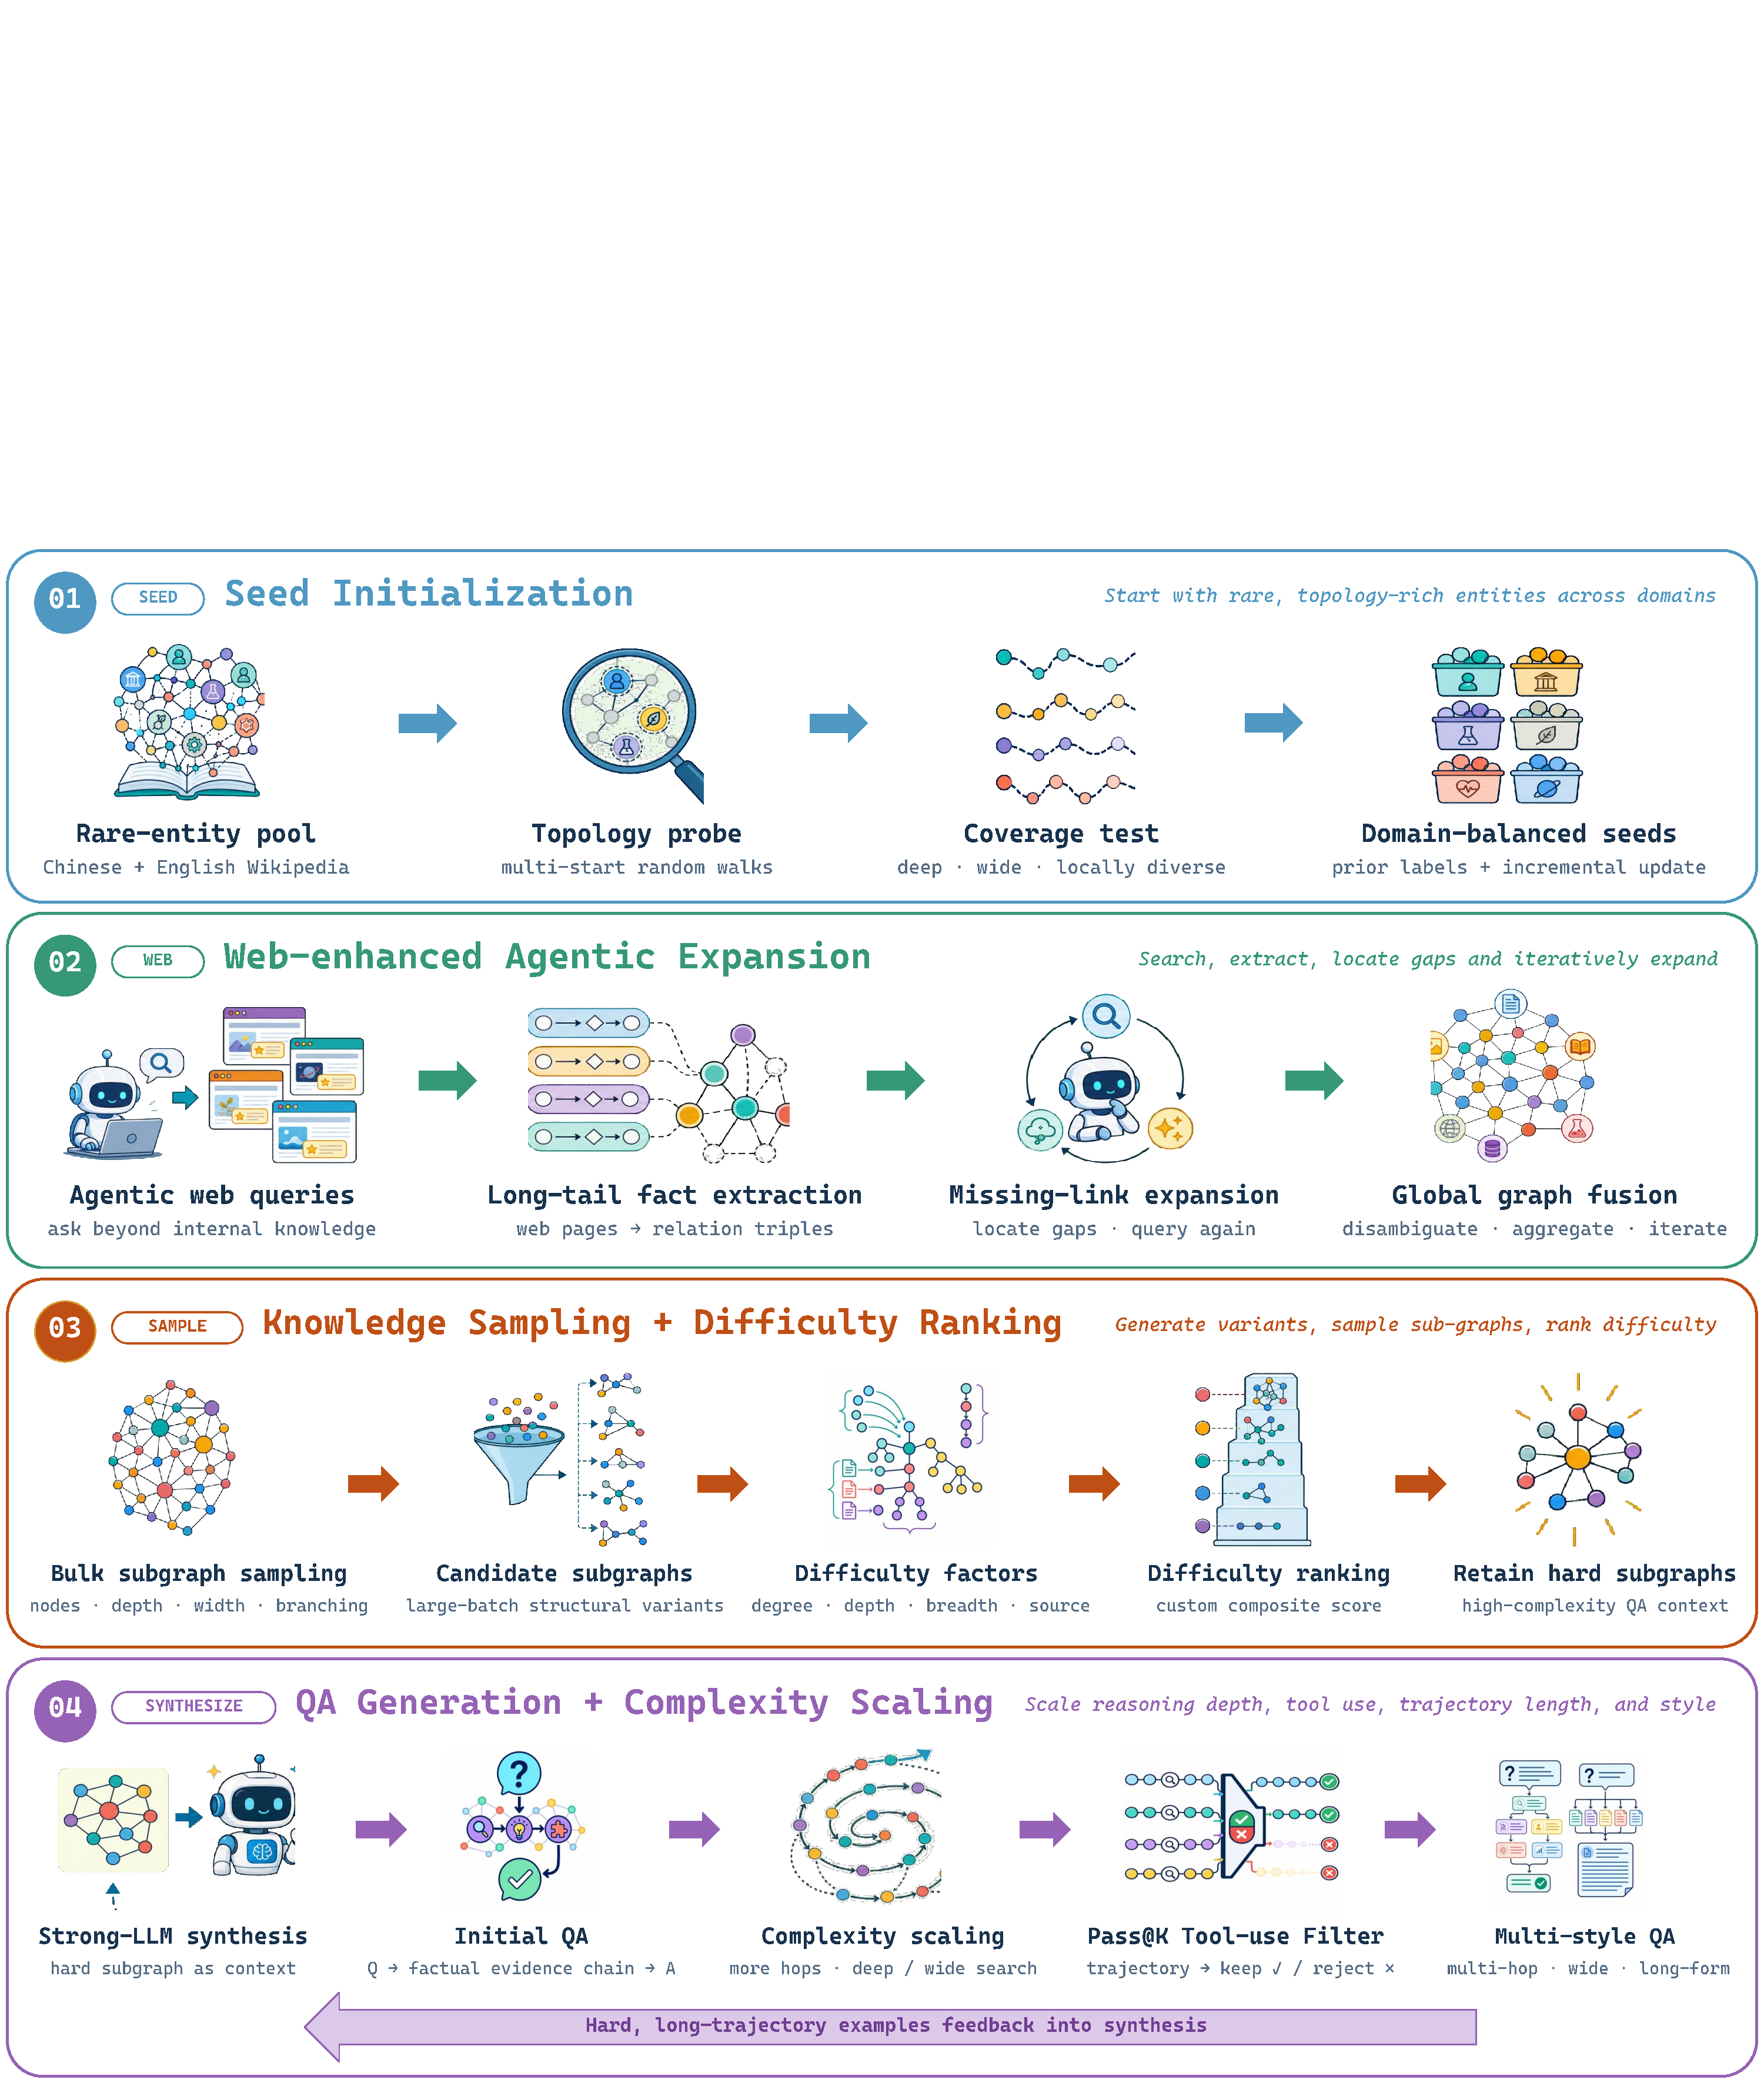
\includegraphics[width=1.0\linewidth]{img/Web_Enhanced_Complex_QA_Pipeline_Visual_Clarity_Optimized_v2.pdf}
    \caption{Overview of the DeepSearch QA Synthesis.}
    \label{fig:deepsearch_qa_synthesis_framework}
\end{figure}

\subsubsection{Seed Initialization}
Seed initialization determines the distribution from which long-horizon search tasks are drawn, and thus critically shapes their difficulty, diversity, and scalability. Instead of sampling at random, we deliberately curate a pool of \emph{long-tail} entities selected along three complementary axes—limited parametric exposure, structural richness, and balanced domain coverage—which we detail below. These entities then seed the subsequent web-enhanced agentic knowledge expansion stage. 

\paragraph{Limited Exposure in Parametric Knowledge.}
Entities that are extensively represented in a model's parametric knowledge may permit shortcut solutions, allowing the model to answer directly from memorization rather than genuine external retrieval. To suppress such shortcuts, we sample long-tail entities from large-scale multilingual knowledge graphs constructed from Wikipedia, prioritizing those with low in-degree and out-degree. Grounding tasks in these less prominent entities substantially increases the likelihood that successful completion requires actively acquiring and integrating external evidence, thereby preserving the retrieval-centric nature of the benchmark.

\paragraph{Sufficient Structural Richness.} 
Rare entities often reside in structurally sparse regions of the knowledge graph, where limited relational context constrains the construction of multi-hop reasoning chains and complex evidence dependencies. To quantify the context-expansion potential of each candidate, we perform multiple randomized graph walks originating from the entity and analyze the topology of the resulting local neighborhoods. Seeds that consistently reach structurally rich subgraphs—characterized by diverse relation types, branching evidence paths, and extended multi-hop connectivity—are assigned higher priority, ensuring that each seed can anchor a sufficiently deep and interconnected reasoning task.

\paragraph{Balanced Domain Coverage.}
Beyond structural complexity, broad topical coverage is essential for scalable task synthesis. Because graph-based sampling tends to concentrate on densely connected domains while overlooking specialized areas, we organize seed entities within a hierarchical domain taxonomy that couples predefined categories with regions discovered dynamically during expansion. Domain-specific sampling quotas are then adjusted on the fly to maintain balanced representation, preventing the resulting task set from collapsing onto a handful of popular topics and instead promoting even coverage across the knowledge landscape.


% \subsubsection{Seed Initialization}
% % Seed initialization determines the distribution from which long-horizon search tasks are constructed and therefore plays a critical role in determining the difficulty, diversity, and scalability of the resulting QA pairs.
% % Seed initialization determines the distribution of long-horizon search tasks and influences the complexity, diversity and scalability of the synthesized QA pairs. \textcolor{red}{To facilitate high-quality task construction, we select long-tail entities that satisfy three criteria: (i) limited exposure in the parametric knowledge of large language models, (ii) sufficient structural richness to support long-horizon knowledge expansion, and (iii) balanced coverage across heterogeneous knowledge domains. These entities serve as the initial seeds for the subsequent web-enhanced agentic knowledge expansion stage.}


% \paragraph{Limited Exposure in Parametric Knowledge.}
% Seeds that are extensively represented in a model’s parametric knowledge may enable shortcut solutions that require little or no external information retrieval. 
% To reduce this shortcut, we sample long-tail entities from large-scale multilingual knowledge graphs constructed from Wikipedia.
% Specifically, we select entities with low in-degree and out-degree. By constructing tasks with these less prominent entities, we increase the likelihood that successful task completion requires acquiring and integrating external evidence.
% % may enable shortcut solutions that require little or no external information retrieval. 
% % To reduce shortcut solving from memorized knowledge, we preferentially sample long-tail entities from large-scale multilingual knowledge graphs derived from Wikipedia. In particular, we prioritize entities with relatively low in-degree and out-degree, as highly connected entities are generally more prominent in pretraining corpora and may expose substantial portions of the solution path through parametric knowledge. Initializing tasks from less prominent entities increases the likelihood that agents must acquire and integrate external evidence rather than rely primarily on information already encoded in model parameters.

% \paragraph{Sufficient Structural Richness.} 
% % In contrast, seeds located in structurally sparse regions may provide insufficient relational context for constructing multi-hop reasoning chains or complex evidence dependencies. We therefore design the initialization procedure to identify entities that jointly minimize parametric-knowledge shortcuts, support structurally rich expansion, and ensure balanced coverage across knowledge domains.

% % Entity rarity, however, is not sufficient to guarantee the construction of challenging search tasks. Many long-tail entities lie in isolated or weakly connected regions of the knowledge graph and therefore provide limited support for complex reasoning chains. To estimate the expansion potential of each candidate seed, we conduct multiple randomized graph walks from the entity and examine the topology of the resulting local neighborhoods. Candidates that consistently reach structurally rich subgraphs — characterized by heterogeneous relation types, branching evidence paths, and extended multi-hop connectivity — are assigned higher priority. This procedure filters out structurally uninformative entities while retaining those that are more likely to support long-horizon search trajectories.
% Rare entities may reside in structurally sparse regions of the knowledge graph, where limited relational context constrains the construction of multi-hop reasoning chains and complex evidence dependencies. 
% To estimate the context expansion potential of each seed, we perform multiple randomized graph walks starting from the entity and analyze the topology of the resulting local neighborhoods. Seeds that consistently reach structurally rich subgraphs—characterized by diverse relation types, branching evidence paths, and extended multi-hop connectivity—are assigned higher priority. 

% \paragraph{Balanced Domain Coverage}
% % In addition to structural complexity, broad topical coverage is necessary for scalable and diverse task synthesis. Without explicit balancing, graph-based sampling can become concentrated in a small number of densely connected domains, while specialized or less represented areas remain under-sampled. We address this issue by organizing seed entities according to a hierarchical domain taxonomy constructed from both predefined vertical categories and knowledge regions incrementally identified during expansion. Each seed is assigned one or more first-level domain labels, and domain-specific sampling quotas are dynamically adjusted to maintain approximately balanced coverage. This mechanism prevents the synthesized tasks from collapsing into a narrow set of popular topics and improves the diversity in both knowledge content and search behavior.
% Beyond structural complexity, broad topical coverage is critical for scalable task synthesis. Graph-based sampling may concentrate on densely connected domains while overlooking specialized areas. To mitigate this bias, we organize seed entities using a hierarchical domain taxonomy that combines predefined categories with regions discovered during expansion. Domain-specific sampling quotas are dynamically adjusted to maintain balanced coverage, preventing tasks from concentrating on popular topics.


% The final seed pool comprises long-tail entities that satisfy three complementary criteria: limited limited exposure to parametric knowledge, sufficient structural capacity for long-horizon expansion, and balanced representation across heterogeneous knowledge domains. These entities provide the starting points for the subsequent web-enhanced agentic knowledge expansion stage.

% \iffalse
\subsubsection{Web-enhanced Agentic Knowledge Expansion}

%\textcolor{red}{
Synthesizing data for search agents requires both broad exploration and deep multi-hop reasoning, demanding comprehensive open-world knowledge coverage and diverse relational connectivity. Existing approaches typically rely on graph traversal over pre-constructed knowledge graphs, restricting exploration to predefined relations and a static knowledge coverage \cite{qwenbai2023qwen,chu2026redsearcher}.
To address these limitations, we develop an explorer agent that autonomously acquires multi-source information and progressively expands a large-scale knowledge graph, which subsequently serves as the basis for the graph sampling stage. 
%}
We give the overview of Web-enhanced Knowledge Expansion in Figure \redref{fig:placeholder}.

%\textcolor{red}{
Starting from a seed entity or an intermediate knowledge subgraph, the explorer agent iteratively expands the graph through a cycle of query generation, web retrieval, knowledge extraction, graph construction, and knowledge-gap discovery. At each iteration, the agent generates queries that go beyond the information already encoded in the current graph. Instead of focusing only on direct attributes of the target entity, it explores broader informative contexts, such as related entities, historical events, organizational affiliations, temporal developments, geographical associations, and cross-domain relations. This iterative process enables the framework to acquire knowledge that is difficult to obtain through local graph traversal alone. Newly extracted entities and relations are continuously integrated into the evolving graph, enabling the search frontier to move beyond local neighborhoods and form richer topologies such as multi-hop chains, branching paths, convergent evidence trails, and densely connected subgraphs.%}


% Starting from the initialized seed entities, our framework performs iterative, web-enhanced knowledge expansion to construct a large-scale, evidence-rich knowledge graph. In contrast to conventional knowledge graph traversal, which is constrained by predefined relations and the coverage of an existing graph, this stage enables an explorer agent to actively acquire open-world information through autonomous search and evidence-guided exploration. The objective is to incorporate knowledge that is unlikely to be fully represented in either the seed graph or the model's parametric memory, thereby improving the diversity, depth, and novelty of the constructed search tasks.

%xiaohan part
% \paragraph{Iterative Agentic Expansion.} 
% Starting from a seed entity or an intermediate knowledge subgraph, the explorer agent performs an iterative agentic expansion process that alternates among query generation, web retrieval, knowledge extraction, graph construction, and knowledge-gap discovery. At each iteration, the agent generates queries that extend beyond the information already represented in the current graph. Rather than retrieving only direct attributes of the target entity, it actively explores a broader range of informative contexts, including related entities, historical events, organizational affiliations, temporal developments, geographical associations, and cross-domain relationships. This exploration enables the framework to acquire knowledge that cannot be reached through local graph traversal alone. The newly extracted entities and relations are continuously integrated into the evolving knowledge graph, allowing it to expand both in depth and breadth across iterations. As the search frontier dynamically evolves, the agent naturally explores diverse expansion trajectories instead of remaining constrained to a single path. Consequently, the iterative expansion process promotes the emergence of increasingly rich topological structures, including multi-hop reasoning chains, branching paths, convergent evidence trails, cross-domain connections, and densely interconnected local subgraphs, thereby constructing a more comprehensive and structurally diverse knowledge representation.


% The expansion process alternates among query generation, web retrieval, knowledge extraction, graph construction, and knowledge-gap discovery. Newly acquired entities and relations are added to the evolving graph, allowing the graph to grow both in depth and breadth. As the search frontier continuously evolves across iterations, the agent naturally explores diverse expansion trajectories rather than remaining constrained to a single expansion trajectory. This process promotes the emergence of complex topological graph patterns, including multi-hop chains, branching paths, cross-domain connections, convergent evidence trails, and densely interconnected local subgraphs.

% Given a seed entity or an intermediate knowledge subgraph, the explorer agent generates queries that extend beyond the information already encoded in the current graph. Rather than retrieving only direct attributes of the target entity, the agent investigates a broader range of potentially informative contexts, including related entities, historical events, organizational affiliations, temporal developments, geographical associations, and cross-domain relationships. This active exploration allows the framework to uncover knowledge that cannot be reached through local graph traversal alone.


\paragraph{Web-guided Knowledge Acquisition.} For each generated query, the agent retrieves evidence from external web pages and extracts candidate factual statements from the returned content. To maximize the informational value of acquired information, the extraction process prioritizes uncommon facts and non-trivial entity relations over frequently repeated surface-level descriptions. Each extracted statement is converted into a structured relation representation consisting of: (1) Source entities, (2) Target entities, (3) Relation types, (4) Textual descriptions, and (5) Supporting evidence references. Relations extracted from each retrieval source are subsequently organized into source-specific local knowledge graphs.



\paragraph{Knowledge-gap Discovery \& Targeted Expansion.} A major challenge is that Evidence retrieved from the open web often yields incomplete local graph structures. For example, an entity may be introduced without sufficient contextual connections, an event sequence may contain missing intermediate steps, or a relationship may be supported only from one direction. To address this issue, we introduce a knowledge-gap discovery mechanism that analyzes the current graph and identifies regions with potentially requiring further exploration. Such regions include sparsely connected entities, unresolved references, incomplete event chains, and partially observed relationship structures. Based on these signals, the agent formulates targeted follow-up queries and initiates additional retrieval rounds to acquire complementary evidence. This mechanism allows the expansion process to progress beyond immediate entity neighborhoods and gradually reveal broader, more coherent evidence networks.

\begin{figure}[!t]
    \centering
    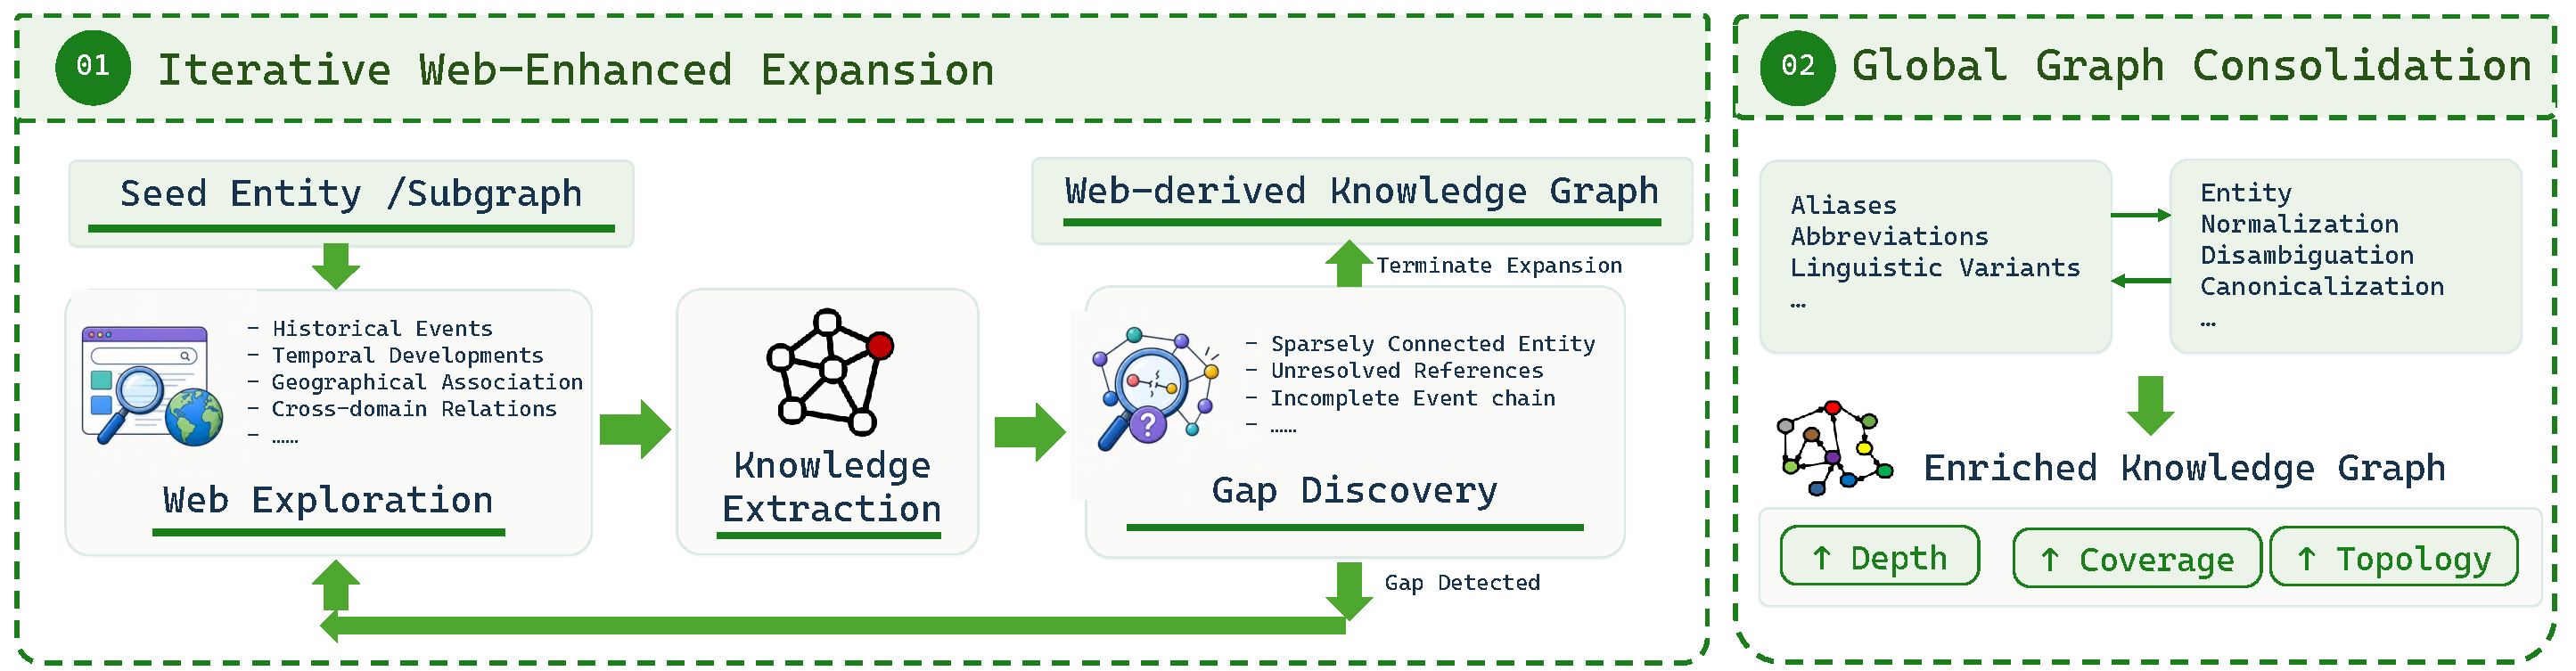
\includegraphics[width=1\linewidth]{img/deepresearch_figure_v2.pdf}
    % 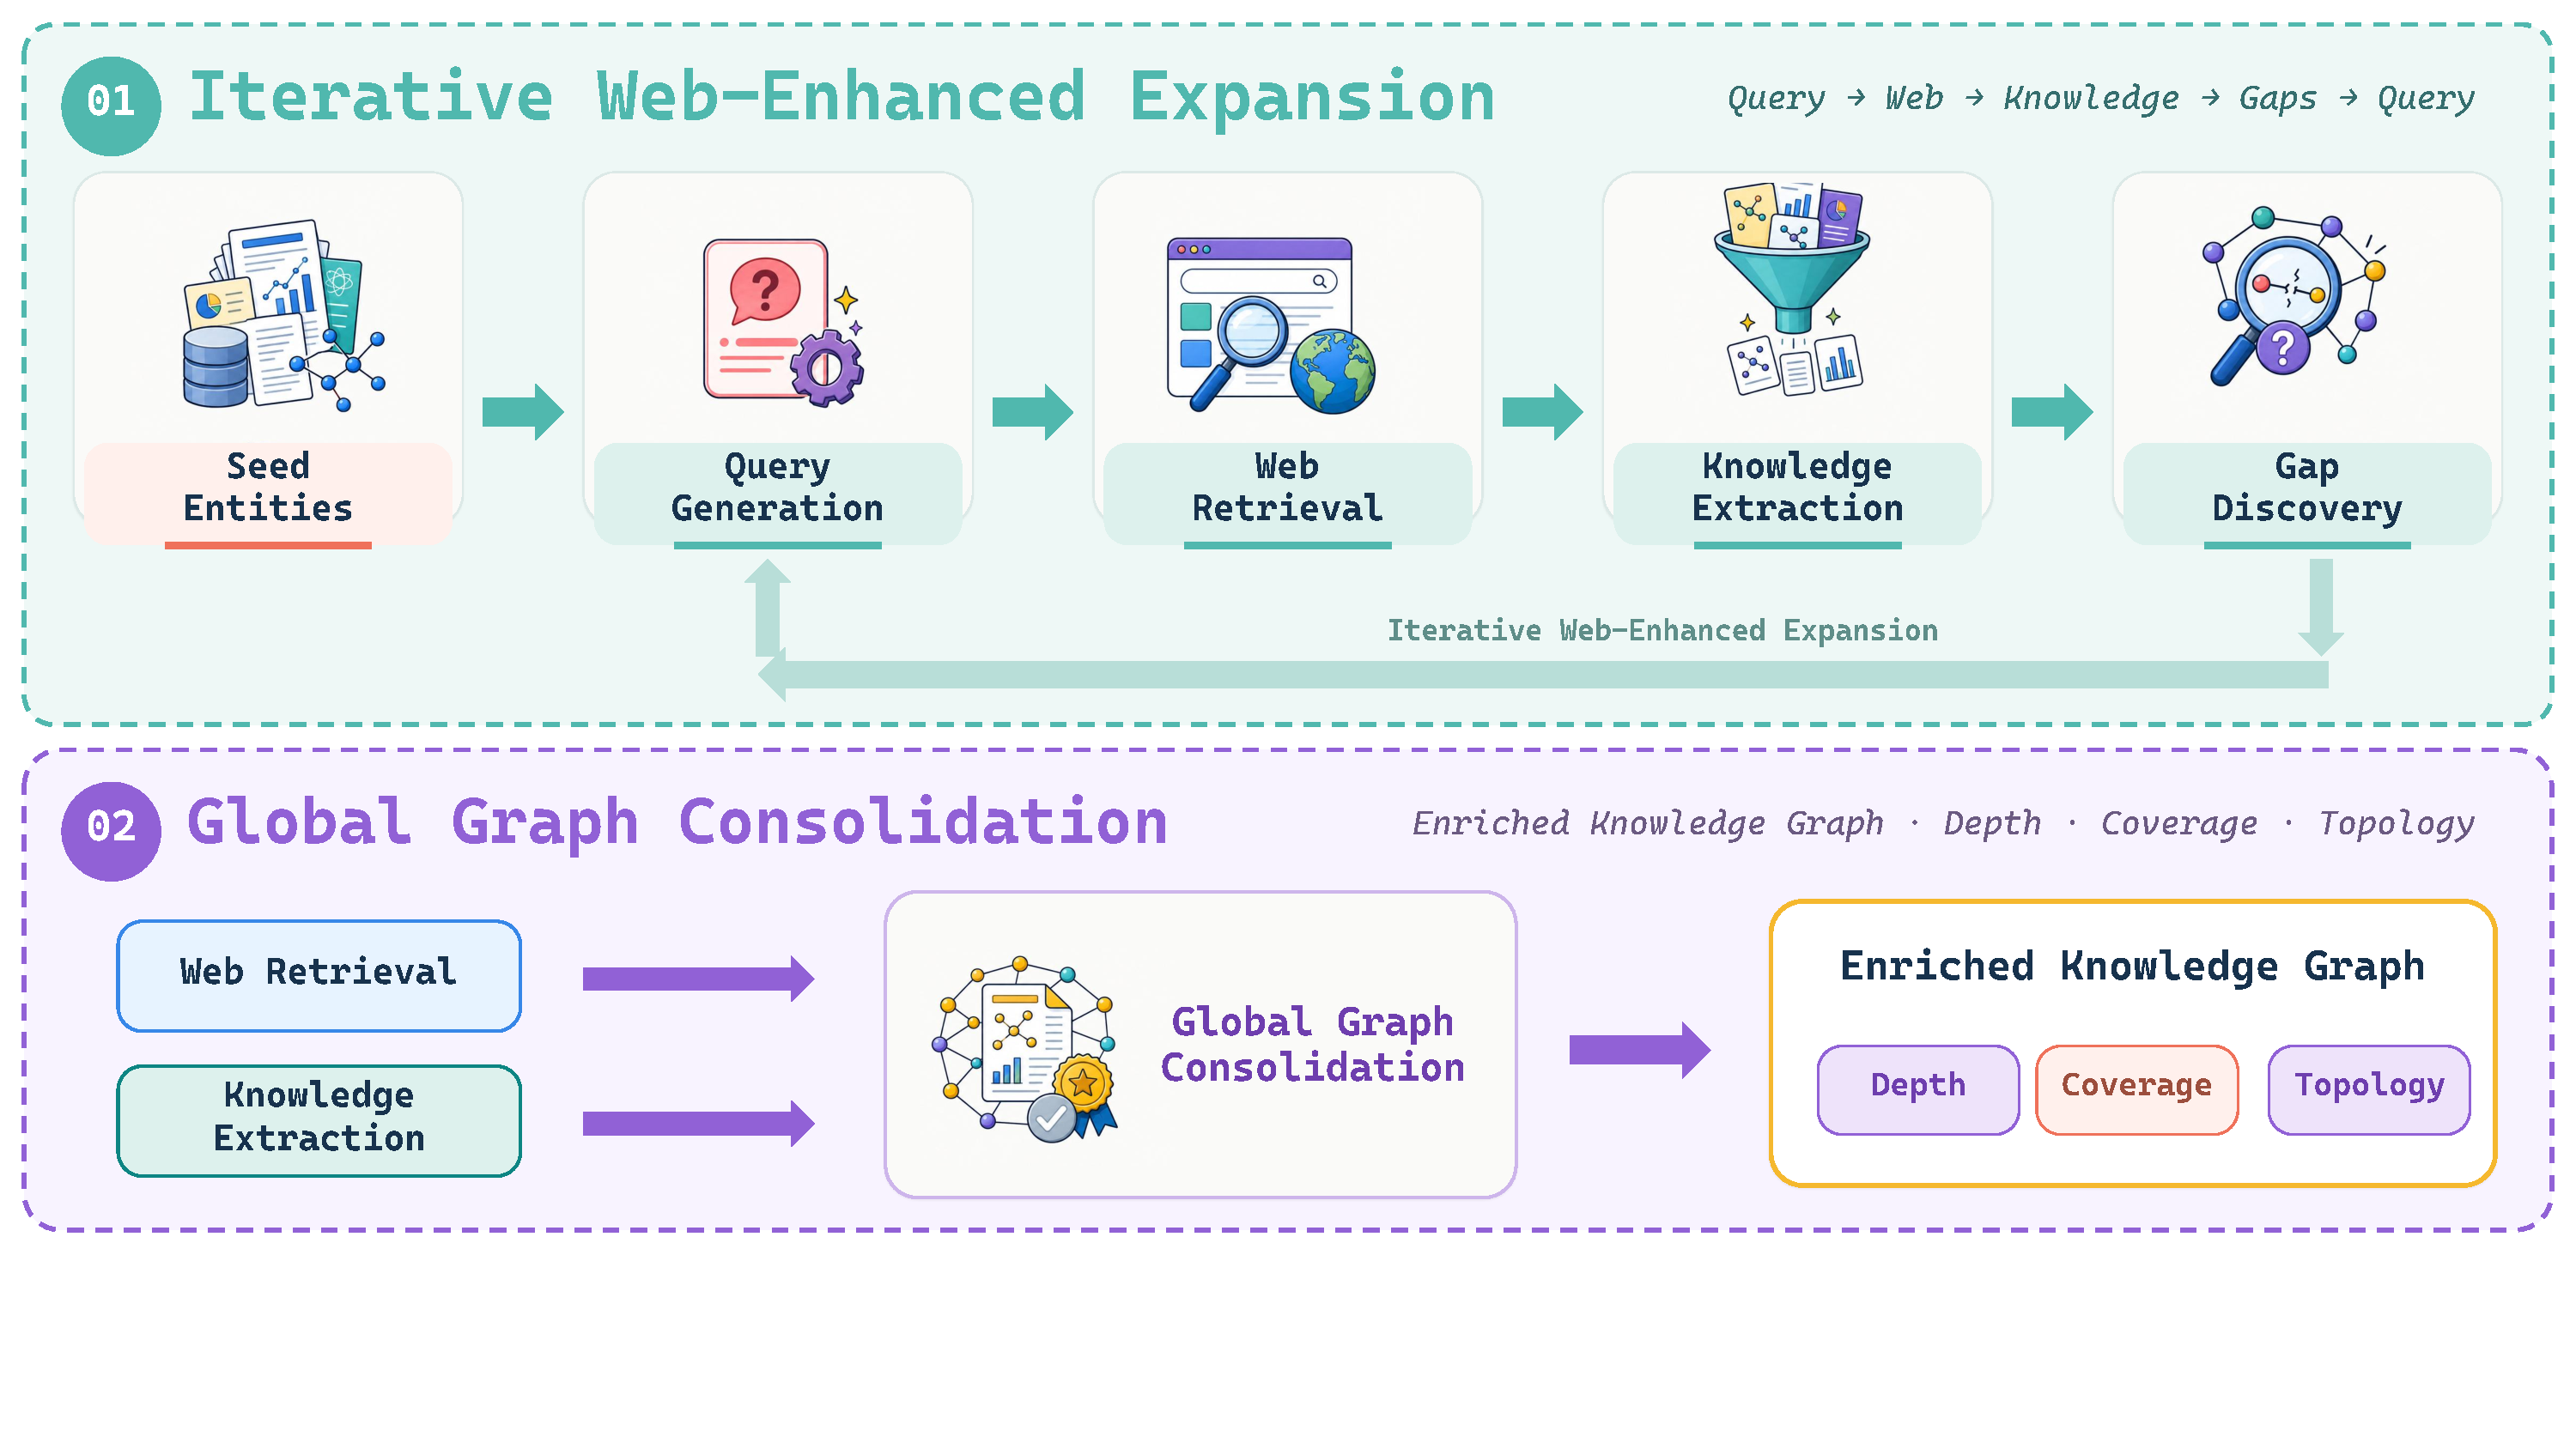
\includegraphics[width=1\linewidth]{img/data_pipeline_restyled_editable_v1.pdf}
    \caption{Procedure of web-enhanced knowledge expansion.}
    \label{fig:placeholder}
\end{figure}

\paragraph{Global Graph Consolidation.} After multiple expansion rounds, knowledge graphs derived from heterogeneous web sources is integrated into a unified global knowledge graph. Since the same real-world entity may appear under different aliases, abbreviations, or linguistic variants, we perform entity normalization, disambiguation, and canonicalization before graph integration. Duplicate or semantically equivalent relations are aggregated while preserving source-level provenance and supporting evidence. The final graph therefore combines evidence acquired across numerous search trajectories and domains, yielding a substantially larger and structurally richer knowledge space than the initial seed graph.


The consolidated global graph provides three properties that are particularly important for long-horizon task synthesis: sufficient depth to support extended multi-step reasoning, broad coverage to enable diverse search trajectories, and heterogeneous local topologies to facilitate the construction of complex search objectives. These properties form the basis of the subsequent knowledge sampling and difficulty-ranking stage.



\subsubsection{Knowledge Sampling with Difficulty Ranking}
After constructing the global knowledge graph, the next challenge is to identify substructures that can yield high-quality, long-horizon search tasks. Although the expansion stage produces a large and heterogeneous graph, many local regions are unsuitable for complex QA synthesis. Some subgraphs contain only shallow relational patterns, whereas others, despite their apparent structural complexity, can be resolved using a small number of highly concentrated evidence sources. We therefore introduce a large-scale subgraph sampling and difficulty-ranking procedure that preferentially retains knowledge regions exhibiting both complex relational structures and dispersed evidence provenance.


Rather than generating questions directly from the entire graph, we first sample extensive subgraphs under configurable structural constraints. Starting from randomly selected root entities, the sampler iteratively expands neighboring nodes while controlling the maximum number of entities, expansion depth, branching width, and node-selection policy at each step. This process yields a large collection of candidate subgraphs with diverse topological structures and evidence distributions. These subgraphs serve as intermediate reasoning templates from which complex search tasks are subsequently synthesized.


% To identify the most challenging candidates, we evaluate the difficulty of each sampled subgraph along two complementary dimensions: structural complexity and evidence dispersion. The former characterizes the complexity of the underlying reasoning structure, whereas the latter estimates the extent to which the supporting evidence must be acquired through multiple independent search paths.
%\textcolor{red}{
To identify the most challenging candidates, we evaluate the difficulty of each sampled subgraph along two complementary dimensions: structural complexity and evidence dispersion. The former characterizes the complexity of the underlying reasoning structure, whereas the latter estimates the extent to which the supporting evidence must be acquired through multiple independent search paths during inference.%}


\paragraph{Structural Complexity.} 
The first component quantifies the topological complexity of the sampled subgraph. Intuitively, reasoning becomes more challenging when entities are embedded in densely interconnected relational structures, and when deriving an answer requires integrating information across deeper and broader dependency paths. %\textcolor{red}{
To capture this difficulty, we characterize the structural complexity of the underlying reasoning graph along three complementary dimensions: connectivity, depth, and width, which respectively reflect relational density, the length of dependency chains, and the breadth of parallel evidence branches.%}
\begin{itemize}[leftmargin=1em, listparindent=\parindent]
\item \textbf{Average Node Connectivity.} For a sampled subgraph $G=(V,E)$, we compute the average node degree:
\begin{equation}
C_{\text{degree}}(G)=\frac{1}{|V|}\sum_{v\in V}\deg(v)
\end{equation}
Higher average connectivity generally indicates denser relational coupling, richer local topology, and a greater diversity of potential reasoning paths. Such structures are more likely to exhibit intersecting evidence chains, alternative traversal routes, and complex dependencies among relational paths, thereby increasing the difficulty of multi-step reasoning.

\item \textbf{Depth Complexity.} We further measure the minimum expansion depth required to reach all sampled entities from the root of the subgraph. A greater depth indicates longer chains of evidence acquisition, suggesting that the final task is more likely to require iterative, multi-step information discovery rather than localized retrieval.

\item \textbf{Width Complexity.} While depth reflects the length of the reasoning chain, width characterizes its breadth. Subgraphs with greater width contain more parallel evidence branches that may need to be explored, compared, and reconciled. Accordingly, a larger minimum width expands the combinatorial space of candidate reasoning trajectories, and reduces the likelihood that a question can be solved through a narrow shortcut.
\end{itemize}
% Together, connectivity, depth, and width characterize the structural difficulty of the underlying reasoning graph.

\paragraph{Evidence Dispersion.}
Structural complexity alone does not necessarily translate into search difficulty. In open-web settings, even a logically complex reasoning structure may remain relatively easy to solve when most of the supporting evidence can be retrieved from only a few search results or source documents. To capture this complementary dimension of difficulty, we introduce \textbf{Evidence Source Dispersion (ESD)}, which quantifies the extent to which the evidence required for solving a question is distributed across heterogeneous information sources.


Each entity and relation in the global knowledge graph is associated with provenance metadata, including the identifier of the search query through which it was discovered and the identifier of its source document. For each sampled subgraph, we aggregate these provenance assignments into source groups and examine the resulting evidence distribution. ESD is then computed using the coefficient of variation of the evidence counts across source groups, thereby characterizing the degree of concentration or dispersion of supporting evidence across queries and documents.


Let $n_i$ denote the number of facts originating from source group $i$. We define:
\begin{equation}
\text{ESD}(G)=\frac{\sigma(n)}{\mu(n)}
\end{equation}
where $\sigma(n)$ and $\mu(n)$ are the standard deviation and mean of the source-frequency distribution, respectively.


Subgraphs with higher evidence dispersion typically require information gathering from multiple independent searches and source documents, rather than from a single highly informative page. These instances are more consistent with realistic deep-search scenarios, in which the process of locating, validating, and synthesizing distributed evidence constitutes a substantial component of the overall task difficulty.


\paragraph{Difficulty Ranking \& Selection.}
The final difficulty score integrates structural complexity and evidence dispersion into a unified ranking criterion. Candidate subgraphs are ranked accordingly, and only the highest-scoring instances are retained for downstream QA synthesis. This selection procedure enriches the generated dataset with long-horizon reasoning structures, multi-source evidence dependencies, and topologically diverse search trajectories.


The retained subgraphs consequently provide a high-quality basis for QA generation, enabling the synthesis pipeline to construct challenging search tasks that require both complex multi-step reasoning and sustained evidence acquisition across heterogeneous sources.



\subsubsection{QA generation with Complexity Scaling}
Given the retained high-difficulty subgraphs, the final stage converts structured knowledge regions into executable DeepSearch QA instances. Rather than merely generating questions that involve multiple facts, we aim to synthesize tasks whose solutions require sustained evidence acquisition, multi-step reasoning, and the resolution of underspecified or obfuscated clues. We therefore introduce a complexity-scaling QA generation procedure that progressively increases task difficulty through subgraph-grounded synthesis, iterative reasoning-chain expansion, and hard-trajectory conditioning.


\paragraph{Subgraph-grounded QA generation.} For each selected subgraph, we prompt a strong LLM to synthesize multiple candidate instances, each comprising a question, an answer, and a factual reasoning chain. The sampled subgraph serves as the factual backbone of the instance, while the strong LLM converts its explicit entities and relations into natural-language search objectives. To prevent direct entity matching and shallow retrieval, the generator is instructed to obfuscate surface-level constants, including entity names, relation descriptions, dates, locations, and numerical values where appropriate. Consequently, the resulting questions typically cannot be solved by directly searching for the answer entity or a single explicit clue. Instead, the solver must identify intermediate targets from indirect descriptions, relational constraints, and partially specified evidence, often through inverse or abductive reasoning.



\paragraph{Factual Reasoning-chain Construction.} Each generated instance is accompanied by a factual reasoning chain grounded in the underlying subgraph. The chain decomposes the solution process into a sequence of evidence-dependent steps, each corresponding to a retrieval operation, clue-resolution step, or inference over retrieved facts. We favor longer chains when they remain factually valid, logically necessary, and free from artificial ambiguity. This design preserves verifiability while requiring the agent to perform long-horizon search and reasoning rather than relying on isolated fact retrieval.



\paragraph{Iterative Complexity Expansion.} Initial generations may still admit retrieval shortcuts or contain reasoning paths of insufficient depth. We therefore apply an iterative enhancement procedure. Given the sampled subgraph and the initially generated QA instances, a strong LLM is prompted to extend, refine, or recombine their factual reasoning chains by incorporating additional entities, relations, and evidence dependencies from the same subgraph. This process transforms relatively direct questions into more demanding search tasks involving broader exploration, deeper dependency chains, and more careful evidence aggregation. An expanded instance is retained only when its answer remains uniquely determined by the supporting evidence and every added reasoning step is factually grounded and relevant to the final solution.


\paragraph{Hard-trajectory-conditioned Generation.} To further increase the lower bound of task difficulty, we incorporate previously synthesized hard examples into the generation process. For QA instances produced in earlier rounds, we collect long-horizon solving trajectories from strong LLM agents and estimate task difficulty using Pass@$K$-based stratification. QA Instances that remain difficult under multiple sampled solving attempts are treated as high-difficulty examples. Their long-horizon trajectories are then sampled as in-context demonstrations for subsequent rounds of QA generation. These demonstrations expose the generator to empirically difficult search patterns, including delayed clue resolution, multi-branch exploration, ambiguous intermediate entities, repeated query reformulation, and the reconciliation of evidence distributed across distant sources. Hard-trajectory conditioning therefore shifts the generation distribution toward instances that are difficult not only according to static graph properties, but also according to observed agent behavior. Consequently, the synthesized tasks place greater demands on long-horizon planning, adaptive search, intermediate-state tracking, and comprehensive evidence integration.



\paragraph{Multi-style QA Synthesis.} In addition to increasing reasoning complexity, we diversify the linguistic form, interaction style, and expected answer format of the synthesized instances. If all questions follow a benchmark-style multi-hop template, a post-trained agent may overfit to a narrow distribution of clue-dense and explicitly compositional inputs. We therefore prompt the generator to synthesize QA instances in multiple styles. Besides complex multi-hop DeepSearch questions, it generates natural and conversational queries whose information needs are less formally specified. Such questions more closely resemble real user queries, in which the intent may be implicit, relevant constraints may be scattered across the prompt, and the solver must determine which evidence is necessary before constructing an answer.



We further diversify the expected response format. In addition to short factual answers, the generator produces paragraph-level answers that require broader evidence aggregation and explanation. These instances may depend less on a single deep reasoning chain and more on wide search ability: the agent must identify multiple relevant sources, reconcile potentially dispersed evidence, and organize the findings into a coherent, evidence-grounded answer. This design complements depth-oriented multi-hop reasoning with breadth-oriented information synthesis. Collectively, the generated data cover a wider range of practical DeepSearch scenarios, including precise fact tracing, ambiguous intent interpretation, broad information gathering, and evidence-grounded answer synthesis.



The final output of this stage is a collection of $\langle Question, Answer, Factual \ Reasoning \ Chain \rangle$ triples with progressively scaled complexity. These instances are grounded in high-difficulty subgraphs, strengthened through iterative reasoning-chain expansion, and further calibrated by hard trajectory contexts. They provide challenging supervision signals for training and evaluating deep search agents.




\subsection{DeepResearch QA Synthesis}
In addition to graph-grounded DeepSearch QA synthesis, we construct a complementary collection of DeepResearch QA pairs from high-quality, long-form research documents. Unlike fact-centric search questions are typically grounded in localized knowledge subgraphs, DeepResearch questions require agents to explore a broader body of literature, reconcile heterogeneous evidence, and produce comprehensive answers comparable to an expert-written survey or or analytical reports. We therefore regard existing high-quality surveys, review articles, research reports, and analytical papers as naturally occurring reference answers for deep research tasks.

The synthesis pipeline comprises two stages: high-quality answer identification and reverse question generation. In the first stage, we collect long-form documents that provide systematic and well-supported syntheses of specific research topics. In the second stage, we apply reverse prompt engineering to infer the underlying research question for which each document would constitute an ideal answer. This process transforms existing expert-authored documents into supervised question–answer pairs, providing valuable training and evaluation data for deep research agents.
We give the overview and final topic distribution of the DeepResearch QA synthesis in Figure \redref{fig:deepresearch_qa_synthesis_framework} and \redref{fig:deepresearch_theme_distribution}. We give QA examples in Appendix \redref{appendix:DeepResearch QA}


\begin{figure}[!t]%[htbp]
    \centering
    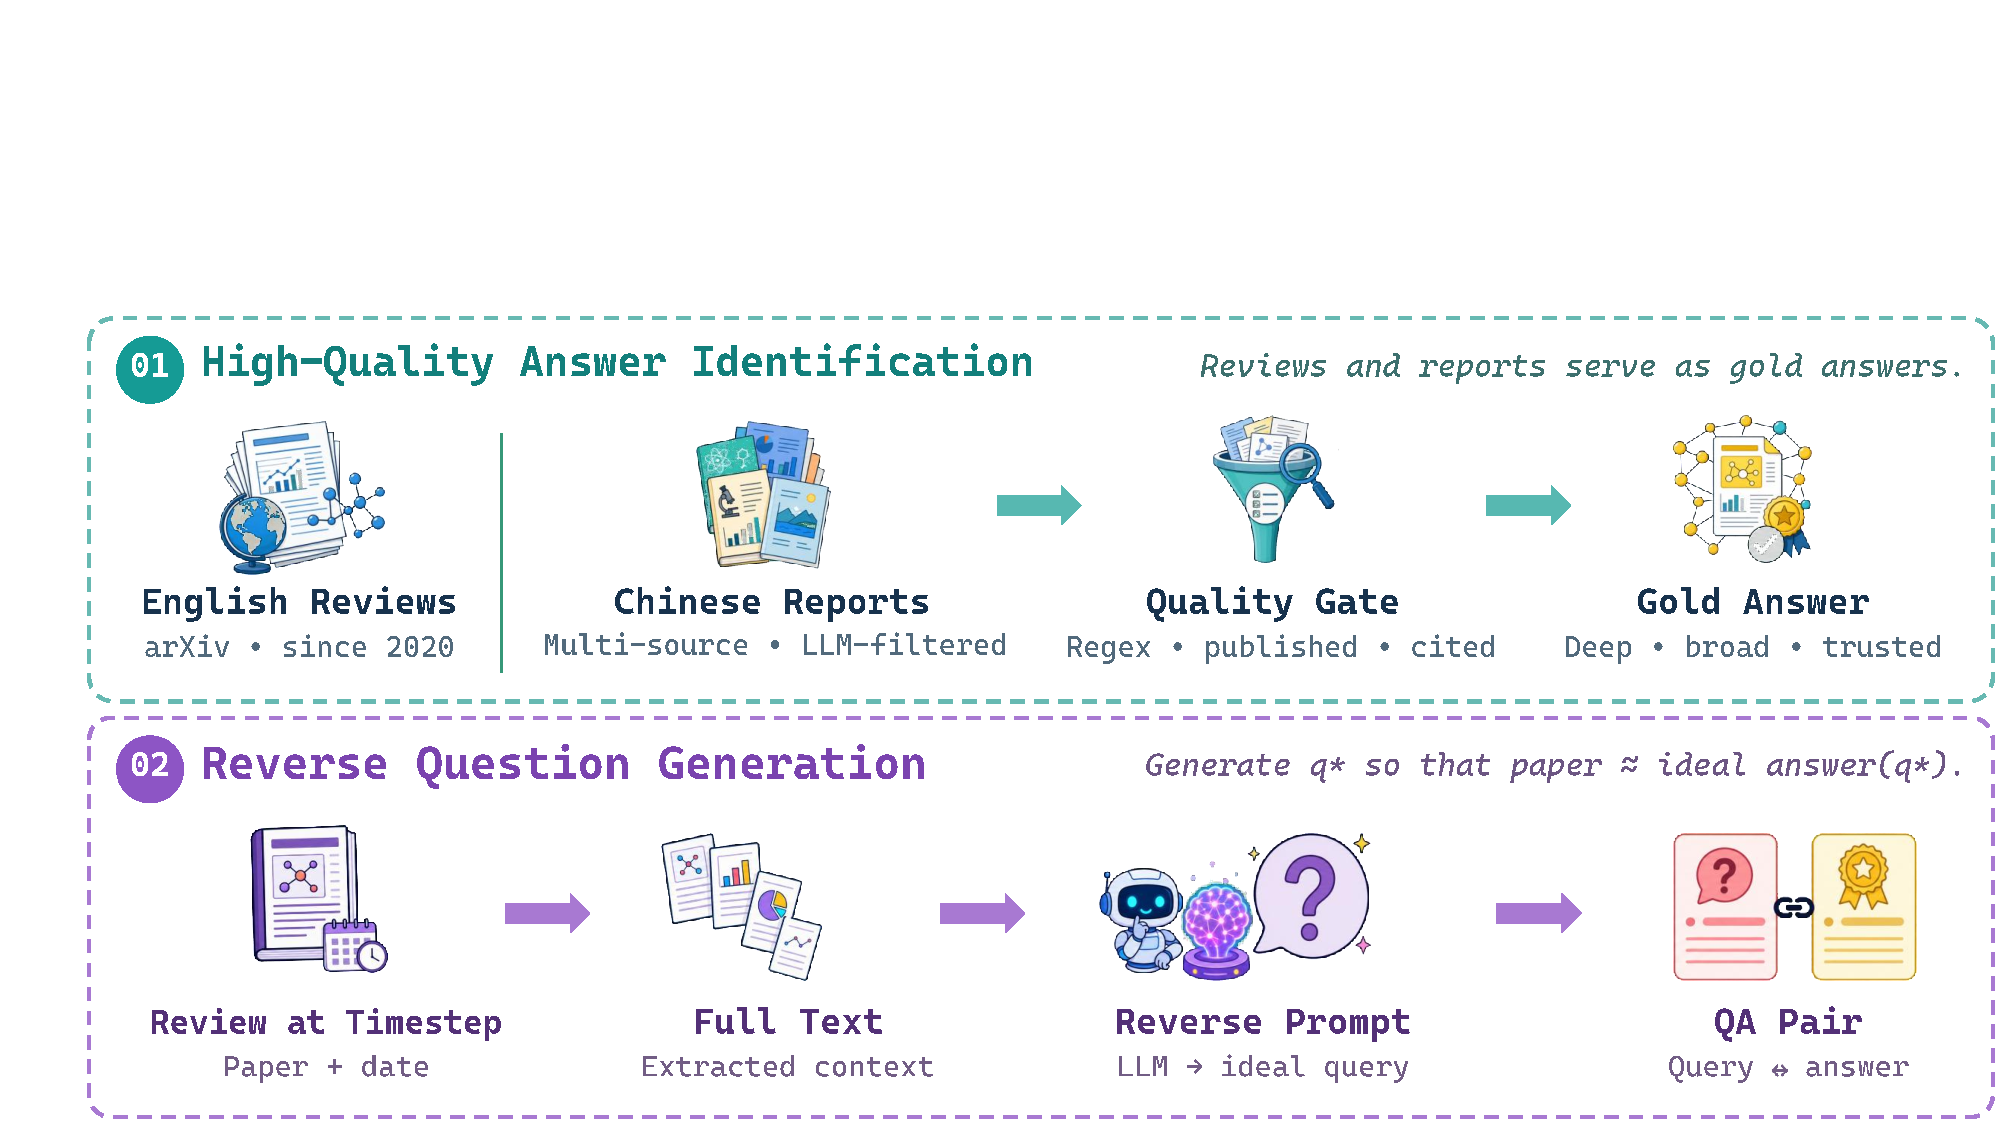
\includegraphics[width=1.0\linewidth]{img/DeepResearch_QA_Synthesis_Model_v1.pdf}
    % 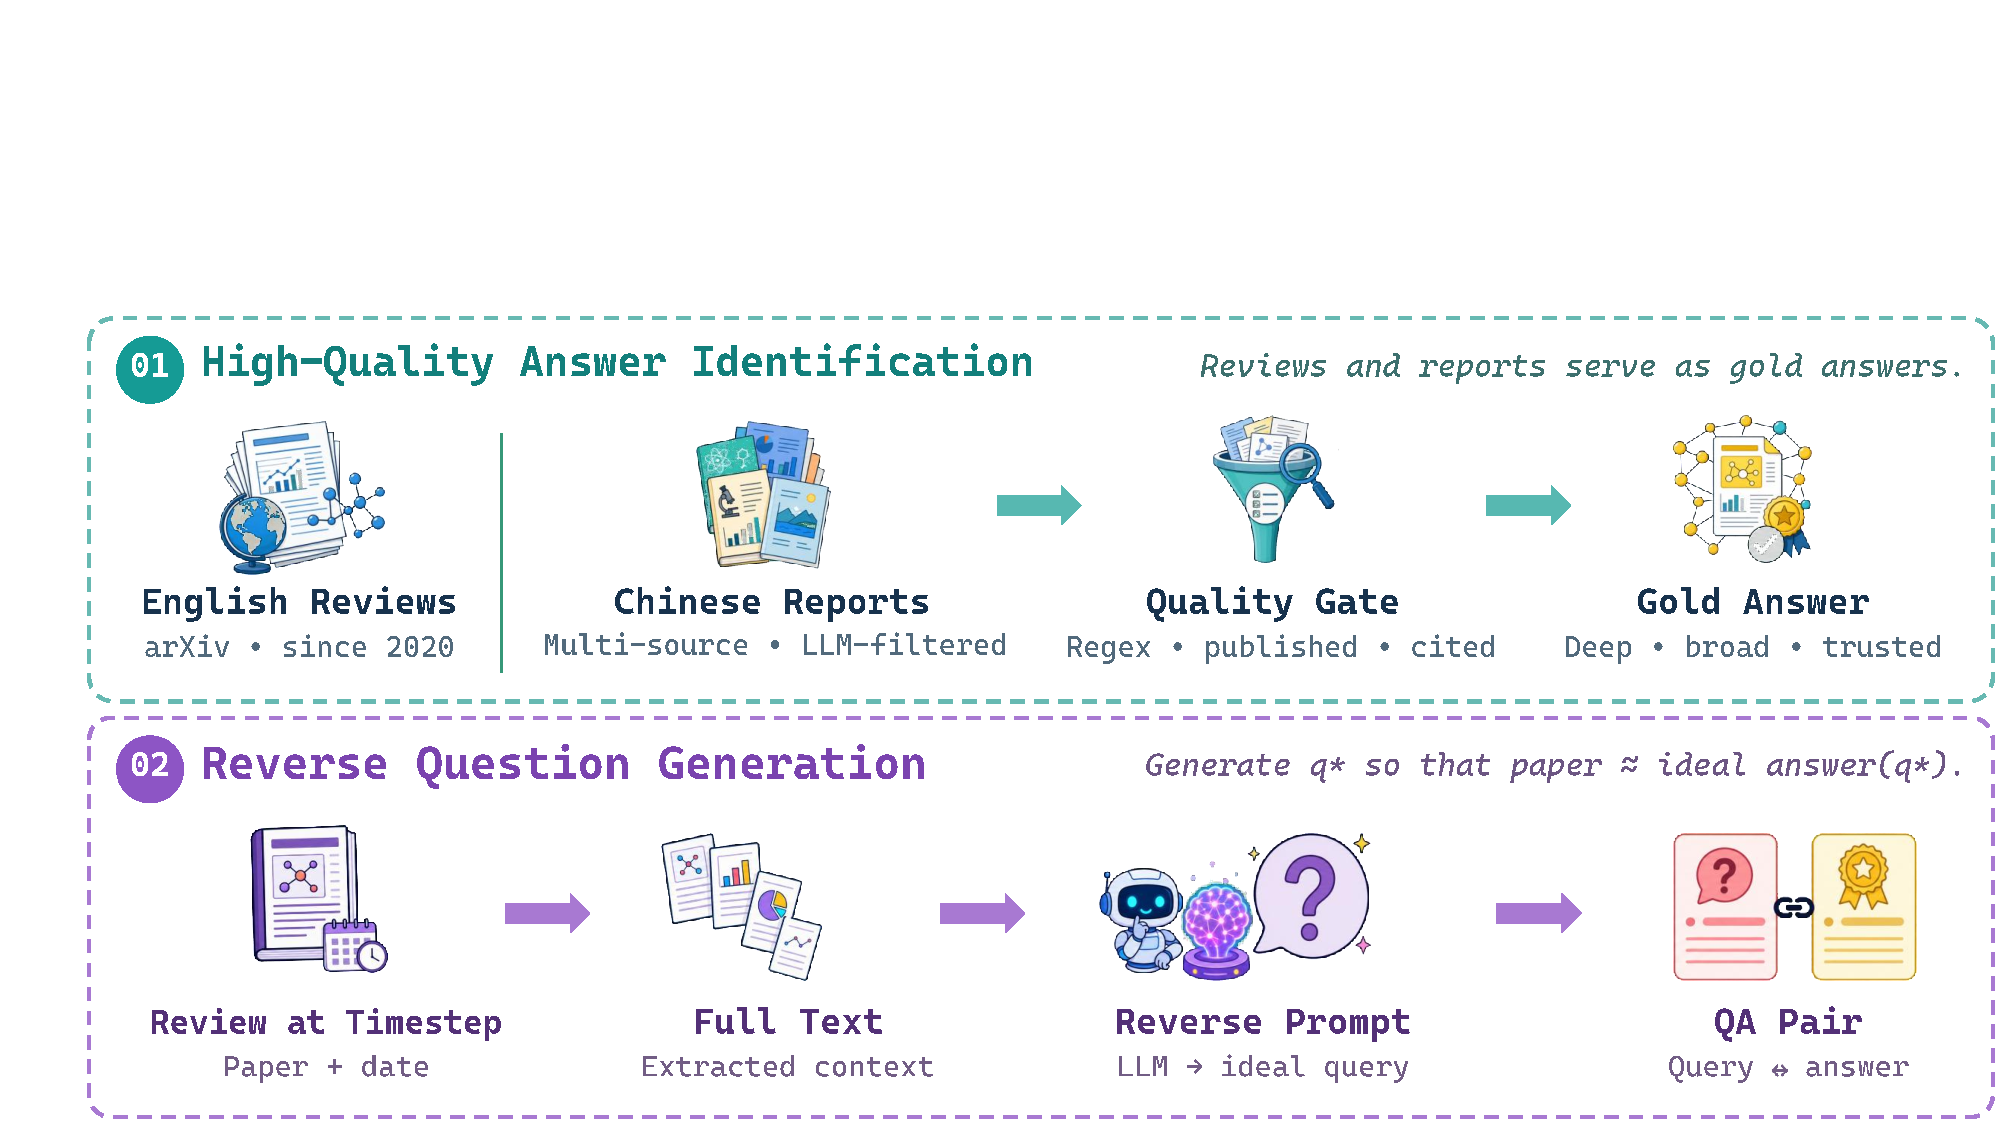
\includegraphics[width=1.0\linewidth]{img/DeepResearch_QA_Synthesis_Model_v1.pdf}
    \caption{Overview of the DeepResearch QA Synthesis.}
    \label{fig:deepresearch_qa_synthesis_framework}
\end{figure}



\subsubsection{High-quality Answer Identification}
The first stage identifies high-quality long-form documents that can serve as reference answers. We focus on surveys, review articles, research reports, and analytical studies because these documents typically synthesize extensive evidence, compare multiple lines of research, and organize information around a clearly defined topic. Unlike short factual answers, such documents more closely reflect the capabilities expected of DeepResearch agents, including sustained information seeking, multi-source integration, critical analysis, and structured synthesis.


For English-language documents, we begin with a comprehensive snapshot of arXiv metadata and retain papers submitted from 2020 onward. Candidate survey-style papers are identified by applying regular-expression filters to their titles, using indicative terms such as "survey", "review", and related expressions. Because title-based retrieval may produce false positives, we subsequently apply additional quality filters. Specifically, when such information is available, we prioritize papers with evidence of peer-reviewed publication, formal acceptance, or substantial citation impact. These signals help distinguish externally validated and influential studies from manuscripts that merely exhibit a survey-like format.


For Chinese-language documents, we collect a broader range of in-depth reports, surveys, technical analyses, and domain-specific research documents from multiple publicly accessible sources. As these documents are distributed across heterogeneous platforms and often lack standardized metadata, conventional metadata-based filtering is insufficient. We therefore employ LLMs to conduct content-level quality filtering. Each document is evaluated in terms of analytical depth, structural coherence, factual density, topical coverage, and the quality of its supporting evidence. Documents that are superficial, predominantly promotional, weakly substantiated, poorly structured, or of limited analytical value are excluded.


Through this process, we obtain a multilingual pool of high-quality long-form answers. These answers cover both academic and applied domains, and provide naturally challenging targets for deep research question generation.



\subsubsection{Reverse Question Generation}
A survey, review, or research report can be regarded as a comprehensive answer to a deep research question under a specific temporal knowledge boundary. Motivated by this perspective, we adopt a reverse question-generation strategy to construct research queries from collected reference documents. Given the publication date and parsed full text of a document, a strong LLM is prompted to infer a research query for which the document would constitute a high-quality reference answer.


Specifically, the model is prompted to formulate a query that reflects the document's central research objective, thematic scope, and expected level of analytical depth. The generated query should not simply request a summary of the source document. Instead, it should define an open-ended research task that naturally requires extensive information retrieval, synthesis, and organization. For example, a survey on retrieval-augmented generation may be transformed into a query requesting a systematic analysis of its major methodological paradigms, evaluation benchmarks, practical limitations, and future research directions.



To preserve temporal consistency between the generated question and its reference answer, the query is conditioned on the publication date or latest update date of the source document. This date serves as the knowledge cutoff for the corresponding research task, ensuring that the expected answer is evaluated against the information available when the reference document was produced. When necessary, the prompt explicitly requires that the scope of the answer be restricted to developments reported before this cutoff date. This design prevents subsequent findings from being incorrectly incorporated into the reference answer and reduces temporal mismatch between questions and answers.



We further introduce constraints to prevent the generated query from revealing the identity of the source document. In particular, the question must not include the exact title, author names, arXiv identifier, report name, or other distinctive surface-level metadata that would enable a solver to retrieve the reference answer directly. Instead, it should express the underlying research objective in natural language. This constraint discourages document-retrieval shortcuts and creates more realistic deep research tasks, in which an agent must independently search for relevant evidence, reconcile information from multiple sources, and synthesize a coherent response.



This stage ultimately produces a collection of document-grounded QA pairs. Each answer corresponds to an existing high-quality survey, review, research report, or analytical document, whereas each question is a reverse-generated deep research query aligned with the document's content and temporal scope. These pairs provide complementary supervision to graph-grounded DeepSearch QA. Graph-based synthesis primarily supports controllable, fine-grained factual reasoning over structured evidence chains, whereas document-based DeepResearch synthesis emphasizes broad topical coverage, long-form evidence integration, and expert-level organization of complex information.

\begin{figure}[!t]%[htbp]
    \centering
    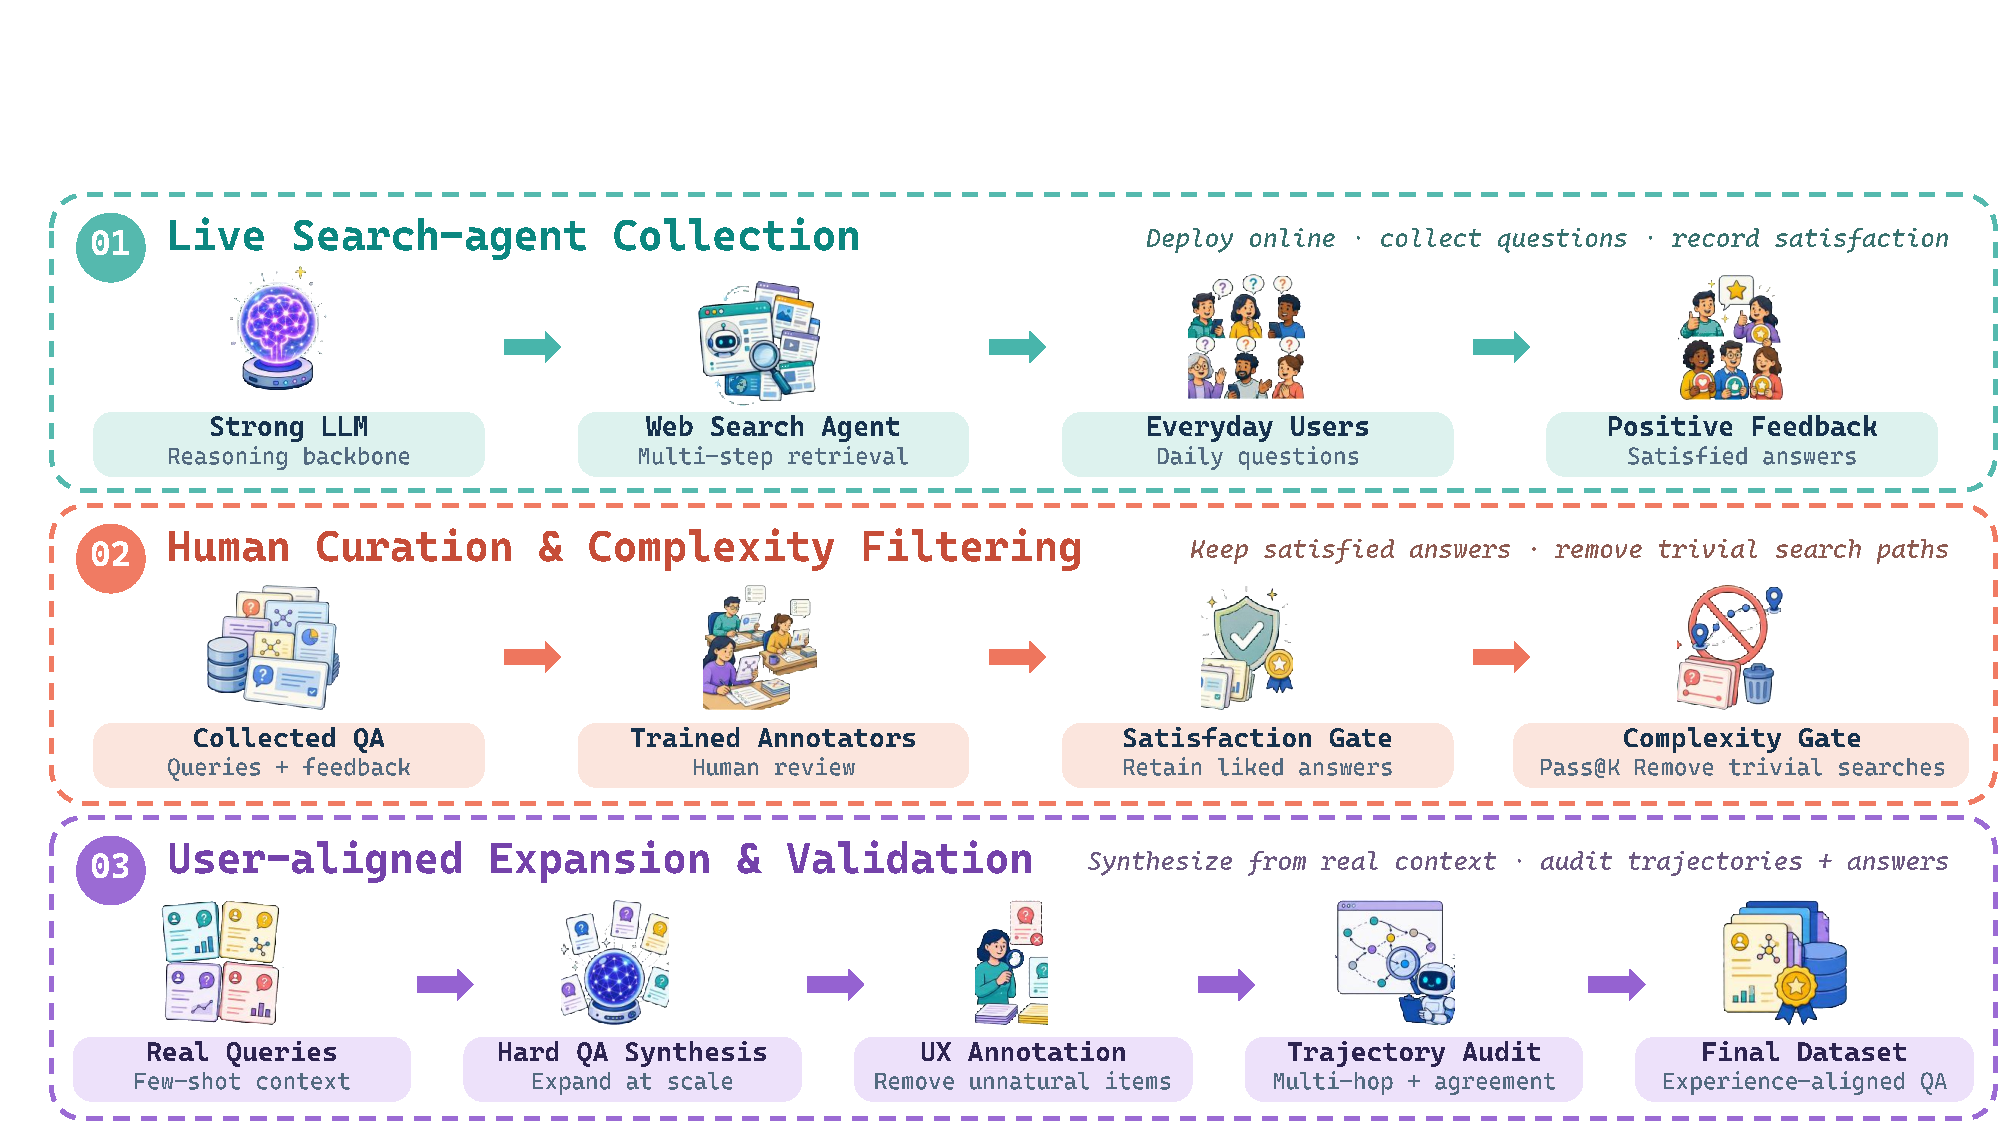
\includegraphics[width=1.0\linewidth]{img/Real-world_User_Experience_QA_Model_v1.pdf}
    \caption{Overview of the Real-world User Experience–oriented QA Synthesis.}
    \label{fig:Real_world_User_Experience_QA_synthesis_framework}
\end{figure}

\subsection{Real-world User Experience–oriented QA}
Although synthetic long-horizon search tasks enable precise control over question difficulty and reasoning structure, they do not fully reflect how users interact with search agents in real-world scenarios. Existing search-agent data synthesis pipelines primarily focus on benchmark-style questions, such as multi-hop reasoning tasks constructed with intentionally obfuscated clues. While such questions are valuable for evaluating search depth and resistance to reasoning shortcuts, they can differ substantially from daily information-seeking needs. Real users often pose open-ended, preference-sensitive, and decision-oriented questions that require broad evidence collection, contextual understanding, and grounded synthesis.


To narrow this gap, we construct a complementary collection of Real-world User Experience-oriented QA data. Our objective is to develop challenging questions that preserve natural user intent, practical decision-making needs, and realistic interaction patterns, while still requiring substantial search depth and breadth. These questions often involve scenarios such as evaluating recently released products, conducting technical comparisons, planning travel, making financial decisions, interpreting policy changes, developing learning strategies, and balancing personalized trade-offs.
For example, a user may ask whether replacing two 27-inch 4K monitors with a single 32-inch 4K monitor would be preferable for programming, spreadsheet work, and occasional gaming, while considering products released or expected around May 2026, cost-effectiveness, workspace constraints, and real-world user feedback. Answering such a question cannot be reduced to a single factual lookup. Instead, it requires temporal awareness, multi-source evidence retrieval, structured comparison, and user-centered reasoning. By incorporating these realistic and decision-intensive queries, this dataset complements synthetic benchmark-style tasks and provides a more direct basis for improving the practical utility of search agents.
We give the overview of the Real-world User Experience–oriented QA synthesis in Figure \redref{fig:Real_world_User_Experience_QA_synthesis_framework}.
We give QA examples in Appendix \redref{appendix:Real-world User Experience–oriented QA}





\subsubsection{User-facing Search Agent Deployment}
We deploy the search-agent inference framework through an online web interface powered by a strong LLM. Rather than interacting with artificially constructed benchmark prompts, users are encouraged to submit natural, daily information-seeking questions. For each query, users can inspect the generated answer and provide feedback on its quality, usefulness, factual accuracy, and overall satisfaction.



This deployment enables the collection of queries that more closely reflect real-world information needs and interaction patterns. Compared with manually designed benchmark tasks, user-generated queries exhibit greater diversity in intent, less standardized phrasing, and more realistic constraints. They often involve underspecified preferences, implicit assumptions, time-sensitive information, multi-objective comparisons, and subjective assessments of utility. These characteristics provide valuable training signals for developing search agents that can generalize beyond rigid benchmark settings and respond effectively to heterogeneous user needs.



\subsubsection{Human Filtering and Quality Control}
After collecting a sufficiently large pool of user queries and associated feedback annotations, we conduct a human-in-the-loop filtering process to construct a high-quality seed set. Multiple trained annotators independently review the collected examples and retain queries for which users indicate satisfaction with the quality and usefulness of the corresponding answers. We exclude examples that are trivial, highly subjective and lack verifiable evidence, or can be resolved through only one or two superficial search steps.



The filtering process is guided by two primary criteria. First, each query should reflect a realistic information need and be formulated in a manner consistent with how users naturally express such needs in practice. Second, answering the query should require substantive search and reasoning, such as retrieving up-to-date information, consulting and comparing multiple sources, synthesizing evidence across documents, or reconciling conflicting claims. This procedure ensures that the retained examples are both representative of real-world user requests and sufficiently search-intensive.





\subsubsection{User-style QA Synthesis}
Although directly collected user queries offer high authenticity, they remain limited in both scale and domain coverage. To broaden the dataset while preserving realistic user intent, we use the collected queries as in-context demonstrations for further synthesis. Specifically, we integrate these examples into the DeepSearch QA Synthesis pipeline described above and prompt a strong LLM to generate additional questions that retain the linguistic style, intent structure, and practical orientation of real user requests, while incorporating the difficulty controls introduced by graph-grounded and search-intensive QA synthesis.



This procedure produces questions that are challenging not only in terms of reasoning complexity, but also from the perspective of real-world information seeking. The synthesized queries commonly involve constrained decision-making, multi-source comparison, recent or evolving information, and nuanced trade-offs between competing objectives. Unlike benchmark-style questions that rely on artificial obfuscation to increase difficulty, these examples are designed to resemble authentic user requests for which accurate and comprehensive answers require substantial search, evidence integration, and contextual reasoning.




\subsubsection{Post-generation Validation}
To ensure data quality, the synthesized user-oriented questions undergo a multi-stage validation procedure. First, human annotators remove questions that do not reflect natural interaction patterns, impose implausible or contrived constraints, or otherwise appear overly artificial. Second, a strong LLM is used to generate search trajectories and candidate answers for each retained question. We discard examples whose solution requires only a shallow search process, whose supporting evidence can be retrieved through a single straightforward query, or whose generated answers are inconsistent across repeated attempts.



This filtering and validation procedure yields a collection of real-world, user-experience-oriented QA examples characterized by three key properties: natural user intent, practical answer utility, and substantial search complexity. The resulting dataset complements the synthetic DeepSearch and document-grounded DeepResearch QA data by grounding search-agent training in realistic usage scenarios. Consequently, the trained agent is encouraged not only to solve formally challenging tasks, but also to provide useful, evidence-grounded answers to the complex and practical questions encountered in real-world interactions.


\subsection{Multi-Stage Task Verification}
The synthetic QA construction process is designed to increase the difficulty of search and reasoning through mechanisms such as clue obfuscation, multi-hop dependency construction, and evidence integration across multiple knowledge sources. Although these mechanisms are effective in producing challenging tasks, they may also introduce noise and reduce data reliability. For example, some generated QA instances may remain solvable without long-horizon search, whereas others may be ill-posed because the question does not uniquely determine the intended answer. In addition, the target answer may be unverifiable, ambiguous, or inconsistent with the available evidence. To ensure that the resulting dataset is both challenging and reliably verifiable, we introduce a multi-stage task verification pipeline.



The pipeline comprises five stages: rule-based and model-based QA cleaning, direct-reasoning verification using a baseline model, agentic tool-use verification using the same baseline model, agentic verification and trajectory synthesis using a strong model, and final trajectory selection. Together, these stages progressively remove invalid or low-quality instances, estimate task difficulty, verify QA consistency and evidence support, and retain high-quality search trajectories for subsequent training.



\subsubsection{QA Cleaning}
We first apply an automated cleaning procedure to the generated QA pairs to remove malformed and low-quality instances. This stage evaluates surface-level quality, language consistency, length constraints, and content validity. Each QA pair must be written in one of the supported languages, such as Chinese or English; instances containing unsupported languages or inappropriate language mixing are discarded. To prevent questions from becoming overly fragmented or unnecessarily complex, each question is restricted to no more than two interrogative sentences. We also impose a maximum answer length, such as 1,000 tokens, to maintain concise reference answers and prevent them from expanding into uncontrolled long-form documents.


We further remove QA pairs that reveal the synthesis process or rely on unavailable construction context. For example, instances containing expressions such as "according to the given text", "in the knowledge graph", or "based on the above information" are excluded, as these template artifacts indicate that the question is not fully self-contained and depends on hidden contextual information. We additionally discard answers that constitute refusals, non-answers, or statements that the question cannot be answered. Together, these filtering criteria ensure that the retained QA pairs are linguistically well formed, self-contained, answerable, and suitable for search-based evaluation.


\subsubsection{Stage-I Verification: Baseline Direct Reasoning}
The first verification stage estimates whether a task can be solved using parametric knowledge alone. For each QA pair, a baseline LLM is prompted to answer the question directly without access to external search tools. To account for stochastic variation in model generation, we independently sample $N$ responses. Each response is then evaluated against the reference answer using an automated answer-matching verifier.


An instance is retained for subsequent verification only if the baseline model fails to produce a correct answer in all $N$ attempts. Such instances are less likely to be solvable through internal knowledge and are therefore more likely to require external information retrieval and multi-step reasoning. By contrast, instances answered correctly in at least one direct-reasoning attempt may contain overly revealing clues, depend primarily on common knowledge, or otherwise lack sufficient search difficulty; these instances are removed or assigned lower priority.


\subsubsection{Stage-II Verification: Baseline Agentic Tool Use}
Failure under direct generation alone does not establish that a task is both valid and well-posed. A question may remain unsolved because it is ambiguous, lacks sufficient supporting evidence, admits multiple plausible answers, or is inconsistent with its reference answer. To distinguish genuinely challenging tasks from invalid ones, we next allow the same baseline model to solve each question using agentic tools. In each of $N$ independent attempts, the model may autonomously invoke search tools, producing complete solution trajectories and final answers.


Let $n$ $\in$ $\{0,1,\ldots,N\}$ denote the number of attempts whose final answers match the reference answer. When $n>0$, at least one valid solution path has been identified under tool-use reasoning. This provides evidence that the question and reference answer are aligned and that the answer can be recovered from external evidence. By contrast, when $n=0$, the instance may either be too difficult for the baseline agent or be invalid because of reference-answer inconsistency, insufficient evidence, ambiguity, or non-unique solutions. Such cases are therefore subjected to stronger verification in the subsequent stage.




The empirical success rate $\frac{n}{N}$ also serves as a preliminary estimate of task difficulty. Instances solved consistently by the baseline agent are regarded as relatively easy, while those with low success rates are more likely to require stronger search, evidence synthesis, and reasoning capabilities. We therefore prioritize difficult candidates for subsequent verification, particularly those satisfying $n$ $\leq$ $\frac{N}{2}$.



\subsubsection{Stage-III Verification: Trajectory Synthesis with a Strong Agent}
In the third stage, we employ a stronger LLM with agentic search tools to verify the difficult candidates retained from Stage II. For each selected QA pair, the strong agent independently attempts to solve the question $N$ times. We denote by $n$ the number of successful attempts for which the agent's final answer matches the reference answer.


If $n>0$, the QA pair is considered both challenging and verifiable. At least one successful trajectory indicates that the reference answer can be recovered from external evidence through a valid search and reasoning process, while also providing empirical support for the consistency of the question--answer mapping. We therefore retain the instance and preserve its successful trajectories as candidate supervision data. If $n=0$, the instance is discarded, as the pipeline cannot reliably establish that the question is solvable or that the reference answer is adequately supported.


This stage serves two complementary purposes. First, it filters out invalid, ambiguous, or unverifiable hard cases that cannot be resolved even by a stronger search agent. Second, it synthesizes high-quality, long-horizon search trajectories that can subsequently be used for supervised fine-tuning, reward-model training, and trajectory-level analysis.

\subsubsection{Trajectory Selection}
A single QA instance may admit multiple successful solution trajectories, but these trajectories are not necessarily equally useful for training. Some trajectories may contain redundant searches, unnecessary detours, or reasoning patterns that are highly similar to those of other trajectories. We therefore introduce a final selection stage in which a LLM serves as a trajectory judger.


For each QA pair, the LLM judger evaluates the successful trajectories according to four criteria: correctness, search efficiency, evidence grounding, and policy diversity. We retain a small subset of trajectories that are concise, well supported by external evidence, and meaningfully distinct from one another. Preference is given to trajectories that exhibit clear search intent, reliable evidence acquisition, and minimal irrelevant exploration, while preserving alternative strategies when multiple valid solution paths exist.



The final verified dataset contains QA instances that satisfy three conditions: they cannot be easily solved through parametric knowledge alone, they are answerable through external search, and they are supported by one or more high-quality agentic solution trajectories. This multi-stage verification and selection procedure improves the reliability, difficulty, and training utility of the synthesized task set.



\section{Agentic Post-training Pipeline}
Our post-training pipeline comprises two sequential stages: supervised fine-tuning (SFT) followed by reinforcement learning (RL). Both stages are constructed from the same underlying dataset, but adopt distinct data curation and sampling strategies. SFT teaches the model to invoke tools appropriately, interpret intermediate observations, and reason about the current state with respect to the overall task objective. RL subsequently refines the learned policy, improving both task performance and behavioral stability during long-horizon search trajectories.


\subsection{Tool Environment}
We equip the search agent with two tools: \textbf{search} and \textbf{visit}. Given a query, the \textbf{search} tool retrieves relevant online results, including titles, URLs, timestamps, and short snippets. The \textbf{visit} tool fetches the content of a target webpage and summarizes it under an explicit information-extraction objective, retaining evidence that is relevant to the agent's current goal.


To ground post-training in realistic interaction conditions, we construct a real-world tool environment backed by production-grade web services. Specifically, we use Serper\footnote{\url{https://www.serper.dev}} as the search backend, Jina\footnote{\url{https://jina.ai}} for webpage crawling, and Qwen3.5-27B for goal-conditioned content summarization. Although this configuration closely reflects real-world deployment, it introduces substantial challenges for post-training, where tool availability, response consistency, and execution stability are essential.


Production APIs are inherently volatile. They may exhibit variable latency, transient request failures, rate and concurrency limits, dynamically changing webpage content, and interference from advertisements or search-engine-optimized content. These uncertain sources can disrupt trajectory construction, reduce the reproducibility of training examples, and introduce considerable variance into online RL.



To mitigate these issues, we develop a robust tool-environment system built around three mechanisms: caching, disaster recovery, and quality enhancement. Together, they expose a stable and consistent tool interface to the agent throughout the post-training process.


\paragraph{Caching Mechanism}
The search tool uses query-level caching with exact matching: each live search writes its query and results to  an Elasticsearch store, and any subsequent identical query is served directly from it. The fetch-and-summarize tool instead caches only the crawling stage, keyed by the webpage URL. When a URL is requested, a cache hit returns the previously crawled page, while a miss triggers a fresh crawl whose result is then stored. Since the goal-conditioned summary is never cached, the same webpage yield distinct summaries under different query goals, yet each URL is crawled at most once.


The search tool employs query-level caching based on exact matching. Each live search stores the query and its corresponding results in Elasticsearch, and subsequent requests containing the identical query are served directly from the cache. By contrast, the fetch-and-summarize tool caches only the webpage crawling stage, using the URL as the cache key. For each requested URL, a cache hit returns the previously crawled webpage content, while a cache miss triggers a new crawl and stores the resulting content for future use. Goal-conditioned summaries are not cached. Consequently, the same webpage can produce different summaries under different information-seeking goals, while each URL is crawled at most once.

\paragraph{Disaster Recovery} 
The disaster-recovery mechanism maintains tool availability when external services experience high latency, rate limiting, or temporary outages, thereby preventing high-concurrency workloads from substantially reducing overall system throughput.

\paragraph{Quality Enhancement}
We apply several internal rules to improve the quality and robustness of tool responses. Specifically, advertisements are filtered from search results, and quotation marks are removed from search queries because they often cause the search API to return empty results.



\subsection{Supervised Fine-tuning}
We construct a ReAct-style scaffold using the available tool set and employ several closed- and open-source models as teachers for trajectory generation, including Qwen3.5-397B, Qwen3.6-Plus and Qwen3.7-max. The maximum context length is set to 256K tokens, without applying additional context-management strategies. To minimize inconsistencies in tokenization and trajectory formatting, all teacher models are selected from the same model family. The teachers are prompted to generate complete ReAct trajectories comprising intermediate reasoning, tool interactions, supporting evidence, and the final answer.
% \footnote{We evaluated several context-management strategies on the BrowseComp benchmark using Qwen3.5-27B, but all resulted in performance degradation. We therefore retain the original 256K context window.}

For each query in our SFT dataset, we perform $K$ independent rollouts and retain only trajectories whose final answers are judged to be correct by DeepSeek-V4-Pro.
The retained trajectories then undergo a series of quality-control filters, discarding trajectory that (i) contains fewer than 3 or more than 100 interaction turns, (ii) exhibits a failed tool-call rate above 20\%, (iii) shows a mismatch between the query language and the response language (e.g., an English response to a Chinese query), or (iv) contains repetitive patterns in its reasoning content. The resulting high-quality trajectories constitute the final corpus for supervised fine-tuning.
% We then apply additional quality-control filters, discarding trajectories that are less than 3 turns and exceed 100 interaction turns, contain more than 20\% failed tool calls, exhibit a mismatch between the query and response languages, such as an English response to a Chinese query, containing repeated pattern in reasoning content. The resulting high-quality trajectories are subsequently used for supervised fine-tuning.



% trajectory synthesis
% rejection sampling
% training objective

% \subsubsection{Data Construction \& Formulation}
% \subsubsection{Training Objective}

\subsection{Reinforcement Learning}
\subsubsection{RL Algorithm}
We adopt the Decoupled Clip and Dynamic sAmpling Policy Optimization (DAPO) algorithm \cite{yu2026dapo} to train our model. For each query-answer pair $(q, a)$ sampled from the data distribution $\mathcal{D}$, the policy is optimized by maximizing the following objective:
\begin{equation}
\begin{aligned}
\mathcal{J}_{\text{DAPO}}(\theta) ={}& \mathbb{E}_{(q,a) \sim \mathcal{D},\, \{o_i\}_{i=1}^{G} \sim \pi_{\theta_{\text{old}}}(\cdot \mid q)} \\
& \left[ \frac{1}{\sum_{i=1}^{G} |o_i|} \sum_{i=1}^{G} \sum_{t=1}^{|o_i|} \min\!\left( r_{i,t}(\theta)\, \hat{A}_{i,t},\; \text{clip}\!\left( r_{i,t}(\theta),\, 1 - \varepsilon_{\text{low}},\, 1 + \varepsilon_{\text{high}} \right) \hat{A}_{i,t} \right) \right] \\
\text{s.t.} \quad & 0 < \left| \left\{ o_i \mid \texttt{is\_equivalent}(a, o_i) \right\} \right| < G,
\end{aligned}
\end{equation}

where the importance sampling ratio and the group-relative advantage are defined as
\begin{equation}        
r_{i,t}(\theta) = \frac{\pi_\theta(o_{i,t} \mid q, o_{i,<t})}{\pi_{\theta_{\text{old}}}(o_{i,t} \mid q, o_{i,<t})}, \qquad
\hat{A}_{i,t} = \frac{R_i - \text{mean}(\{R_i\}_{i=1}^{G})}{\text{std}(\{R_i\}_{i=1}^{G})}.
\end{equation}

Here $\hat{A}_{i,t}$ is the normalized advantage shared across all tokens of response $o_i$, and $R_i$ denotes the reward assigned to the $i$-th response.
We use the decoupled clipping range where $\varepsilon_{\text{low}}=0.2$ and $\varepsilon_{\text{high}}=0.28$.

% \paragraph{Clip-Higher.} The clipping range is decoupled into a lower bound $\varepsilon_{\text{low}}$ and a higher bound $\varepsilon_{\text{high}}$. Raising $\varepsilon_{\text{high}}$ leaves more room for increasing the probability of low-probability (exploration) tokens, which mitigates entropy collapse and preserves the diversity of generated samples, while a relatively small $\varepsilon_{\text{low}}$ avoids suppressing token probabilities toward zero.

% \paragraph{Dynamic Sampling.} Prompts whose responses are all correct or all incorrect yield a zero group-relative advantage and therefore contribute no gradient. As enforced by the constraint above, we over-sample and filter out such prompts, keeping only those with accuracy strictly between $0$ and $1$, so that every batch retains an effective gradient signal and a consistent number of prompts.

% \paragraph{Token-Level Policy Gradient Loss.} Unlike the original sample-level loss in GRPO, the loss is aggregated at the token level (note the normalization by $\sum_{i=1}^{G} |o_i|$ rather than per-sample averaging). This ensures that longer responses contribute proportionally to the gradient and that desirable or undesirable patterns are reinforced or penalized consistently regardless of response length.

% \paragraph{Overlong Reward Shaping.} To reduce reward noise from truncated samples, a length-aware penalty is added to the rule-based reward. Given a maximum length $L_{\text{max}}$ and a soft punishment cache $L_{\text{cache}}$, the length penalty is defined as
% \begin{equation}
% R_{\text{length}}(y) =
% \begin{cases}
% 0, & |y| \le L_{\text{max}} - L_{\text{cache}}, \\[4pt]
% \dfrac{(L_{\text{max}} - L_{\text{cache}}) - |y|}{L_{\text{cache}}}, & L_{\text{max}} - L_{\text{cache}} < |y| \le L_{\text{max}}, \\[6pt]
% -1, & |y| > L_{\text{max}}.
% \end{cases}
% \end{equation}

% Following the original work, we also remove the KL-divergence penalty term, since the long chain-of-thought policy is expected to diverge substantially from the initial model, making the reference-policy constraint unnecessary.

\subsubsection{Rollout Trajectory Analysis System}
In our experiments, we developed an automated trajectory analysis system to inspect reinforcement learning rollouts and guide the refinement of reward functions, training strategies, and experimental configurations. The system consists of two complementary components: (1) a self-evolving Judge Auditor that detects unreliable evaluation decisions and potential reward-hacking behaviors, and (2) a Tool-Behavior Diagnostic System that compares positive and negative trajectories with respect to tool-call validity, repetitive behavior, failure patterns, truncation, and context utilization.


\begin{figure}[!t]
    \centering
    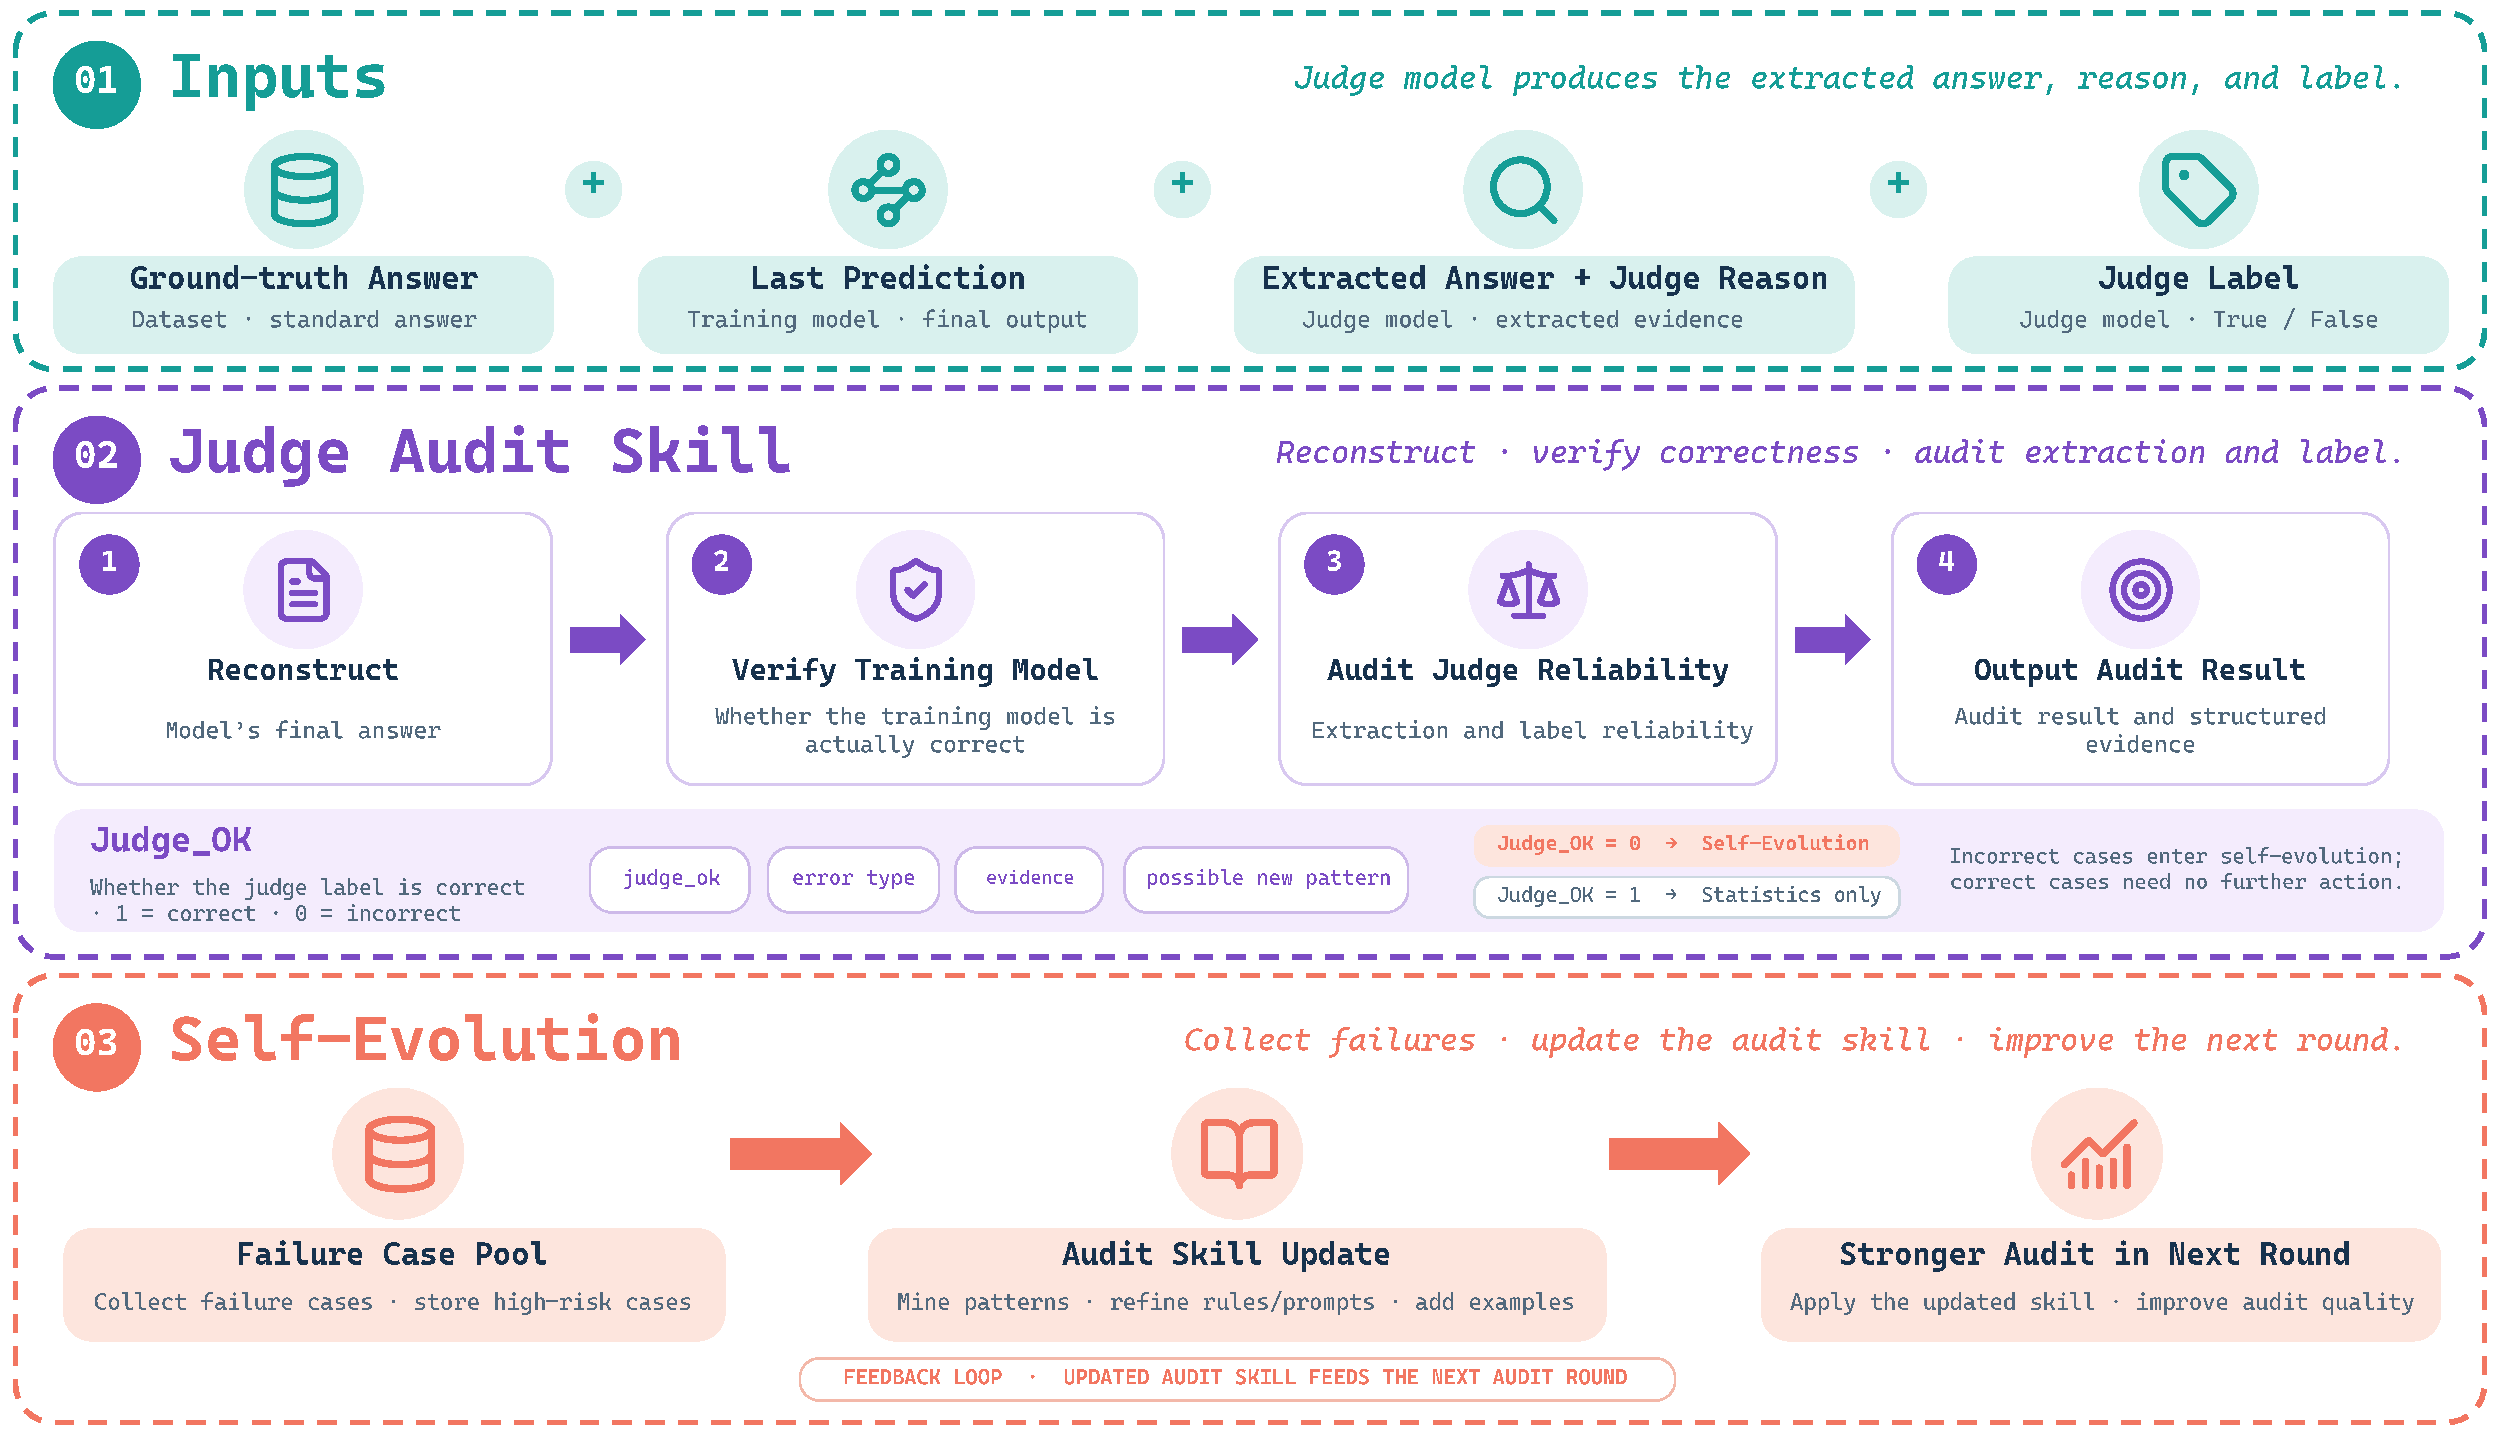
\includegraphics[width=1.0\linewidth]{img/judge_audit_skill_model_figure_optimized.pdf}
    \caption{Overview of the Self-Evolving Judge Auditor.}
    \label{fig:judge_audit}
\end{figure}

\textbf{Self-Evolving Judge Auditor.}
This module identifies potential reward-hacking behaviors to improve training stability and the reliability of reward signals. Because policy behaviors evolve throughout training and may differ substantially across experimental configurations, it is impractical to enumerate all hacking patterns using fixed rules. We therefore introduce a self-evolving auditing mechanism that maintains an external \emph{Audit Skill}, which consolidates auditing criteria, known failure patterns, decision rules, and representative examples. After each experiment, newly identified errors and reward-hacking strategies are incorporated into the Audit Skill, thereby forming a closed-loop process of trajectory auditing, failure discovery, and skill refinement, as illustrated in Fig. \redref{fig:judge_audit}.
To ensure reliable evolution, we construct a stress-test suite consisting of three components: a frozen regression set containing previously resolved failures, an adversarial set comprising manually designed or LLM-generated hacking cases, and a clean control set of normal trajectories. An updated Audit Skill is accepted only if it achieves at least $95\%$ recall on hacking cases, maintains a false-positive rate below $5\%$ on clean samples, obtains a Macro-F1 score above $90\%$, and introduces no more than a one-percentage-point performance regression relative to the latest stable version. Otherwise, the update is rolled back, revised based on the identified failure cases, and subjected to another round of evaluation.


\begin{figure}[!t]
\centering
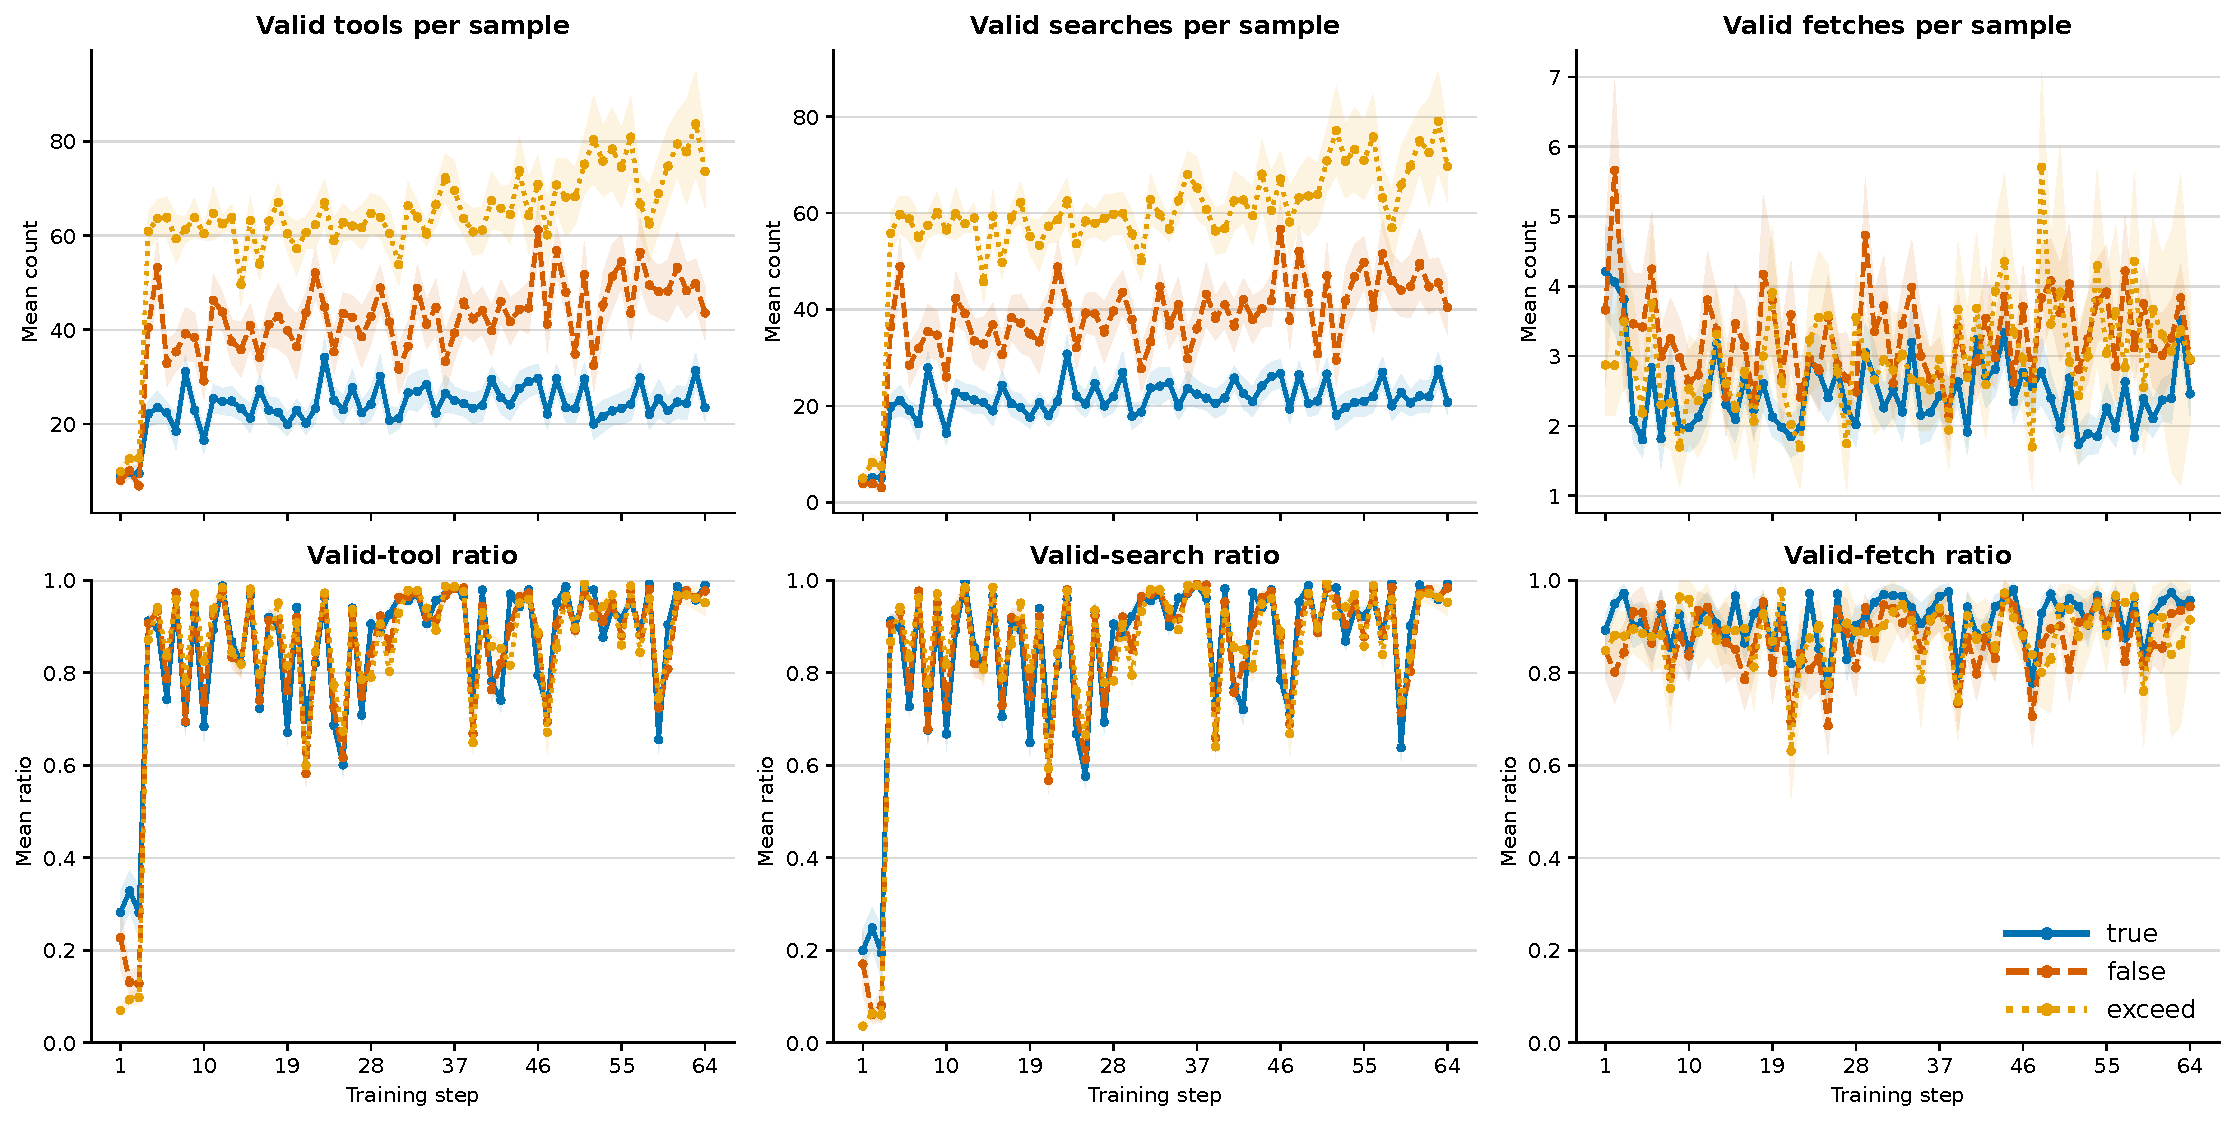
\includegraphics[width=1.0\linewidth]{img/combined.pdf}
\caption{Tool-use curves over training steps for rollout trajectories. A valid tool call is defined as a successfully executed invocation that returns a meaningful result. The top three plots show the average number of valid tool calls, while the bottom three show the proportion of valid tool calls.}
\label{fig:combine}
\end{figure}

\textbf{Tool-Behavior Diagnostic System}.
Beyond diagnosing reward-hacking behaviors at the outcome level, we develop a trajectory-level diagnostic system to systematically analyze tool-use behaviors. The system focuses on two major categories of problematic rollouts: overlength trajectories that exceed the context-window limit without producing a valid final answer, and trajectories that are ultimately judged to be unsuccessful. The system integrates LLM-based semantic analysis, tool-usage statistics, and rollout-tree structural analysis to enable fine-grained attribution of trajectory failures and to provide actionable guidance for optimizing training.
For example, as illustrated in Fig. \redref{fig:combine}, comparisons of the number and proportion of valid tool calls across trajectory categories reveal a persistent \emph{over-searching} pattern in the policy model. In particular, many overlength trajectories arise from excessive, repetitive, and low-yield search behavior, rather than from failures in the external environment. Motivated by this finding, we introduce a behavior-specific penalty for redundant and unproductive tool use, rather than simply masking all overlength samples during training. This strategy retains useful supervision from long yet informative trajectories while explicitly discouraging inefficient search loops.



\subsection{Composite Reward Design}
In long-horizon agentic systems, performance depends on both the correctness of the final answer and the quality of the intermediate reasoning and tool-use trajectory. Therefore, we employ a hybrid reward modeling framework that combines \textbf{outcome-level supervision} and \textbf{process-level supervision}. The overall reward is formulated as:
\begin{equation}
R = R_{\text{outcome}} + \lambda_1 R_{\text{format}} + \lambda_2 R_{\text{turn}}
\end{equation}
where $R_{\text{outcome}}$ measures semantic correctness of the final answer, while process rewards $R_{\text{format}}$ and $R_{\text{turn}}$ regularize structured tool usage and interaction efficiency.

Compared to purely outcome-driven approaches, this decomposition offers several key advantages:
\begin{itemize}[leftmargin=1em, listparindent=\parindent]
\item \textbf{Improved Credit Assignment}: Process-level rewards provide dense, step-wise feedback throughout the trajectory, which reduces the variance of policy gradient updates and leads to more stable optimization.

\item \textbf{Tool-use Reliability}: Format constraints enforce strict compliance with tool invocation schemas, preventing malformed operations that would otherwise cause execution failures.
% format constraints enforce strict compliance with tool invocation specifications, preventing invalid or malformed operations that would otherwise lead to execution failures. This ensures that intermediate actions remain executable and consistent with predefined tool schemas.

\item \textbf{Compute Efficiency Control}: Turn-level rewards explicitly regulate the reasoning budget, discouraging excessively long interaction loops and mitigating unbounded or redundant information-gathering behavior.
\end{itemize}

Overall, this hybrid reward architecture enables stable reinforcement learning in complex multi-step agent environments where both correctness and interaction quality are critical.


% \subsubsection{Outcome Reward: Hybrid Rule-First Evaluation with LLM Judge Fallback.}
\subsubsection{Outcome Reward}
The outcome reward follows \textbf{rule-first, judge-fallback} paradigm that combines deterministic rule-based verification with LLM-based semantic evaluation. Rule-based evaluation provides high-precision, deterministic correctness but is limited by the expressiveness of hand-crafted rules. In contrast, LLM-based evaluation provides flexible semantic evaluation, enabling robust assessment of paraphrases, multilingual expressions, and other semantically equivalent variations, albeit with lower reward stability.

% A key component of our framework is the design of the outcome reward, which follows a \textbf{rule-first, judge-fallback} paradigm. 
% Specifically, we do not treat rule-based verification and LLM-based judgment as independent or competing signals; instead, they form a complementary hierarchical evaluation pipeline.

Given a predicted answer $y$ and reference solution $y^{*}$, we first apply deterministic rule-based verification. These rules include exact match, numerical consistency, set equality, or other task-specific symbolic validations. Formally:
 % structured equivalence checking, 
\begin{equation}
R_{\text{rule}} =
\begin{cases}
1, & \text{if } \text{Verify}_{\text{rule}}(y, y^{*}) = \text{True} \\
\varnothing, & \text{if rule-based verification is inconclusive}
\end{cases}
\end{equation}
The verifier returns an \emph{inconclusive} result when deterministic rules cannot reliably determine correctness. This typically occurs due to (i) semantically equivalent paraphrases, (ii) entity aliasing (e.g., multiple valid names for the same entity), or (iii) multilingual and formatting variations.
In such cases, an LLM judge is invoked as a fallback to evaluate the correctness of the predicted answer and the reference:

% Importantly, the rule system may return an \textit{inconclusive} result when it fails to cover certain cases. This is common in practice due to several factors, including:
% (i) limited rule coverage,
% (ii) lack of robustness to paraphrased or semantically equivalent answers,
% (iii) aliasing phenomena (e.g., multiple valid names for the same entity),
% (iv) multilingual or formatting variations that are not explicitly encoded in rules.
% In such cases, we invoke an LLM-based judge as a fallback mechanism. The judge evaluates semantic equivalence between the model output and the reference:

\begin{equation}
R_{\text{judge}} = \text{LLM}(query, y, y^{*}) \in [0, 1]
\end{equation}

% The final outcome reward is defined as:

% \begin{equation}
% R_{\text{outcome}} =
% \begin{cases}
% 1, & \text{if } R_{\text{rule}} = 1 \\
% R_{\text{judge}}, & \text{if } R_{\text{rule}} \text{ is inconclusive}
% \end{cases}
% \end{equation}

% \paragraph{Rationale.}
% This design reflects a principled trade-off between precision and coverage. Rule-based verification provides high-precision, deterministic correctness signals when applicable, ensuring stable and noise-free supervision. However, its applicability is inherently limited by the expressiveness of hand-crafted rules. The LLM judge complements this limitation by providing a flexible semantic evaluator capable of handling paraphrases, aliasing, and cross-lingual equivalence.

% Compared to a naive mixture-of-experts reward aggregation, this hierarchical design has two advantages: (i) it avoids diluting strong rule-based signals with noisy learned judgments when rules are applicable, and (ii) it ensures fallback coverage in all cases where explicit verification is unavailable. As a result, the outcome reward maintains both reliability and generality across heterogeneous task distributions.



\subsubsection{Process Reward}


While outcome rewards supervise final answer correctness, they provide limited guidance on intermediate reasoning and tool usage quality. To address this, we introduce process-level rewards that explicitly regularize both \textbf{tool invocation validity} and \textbf{interaction efficiency} in agent trajectories.

\paragraph{Format Reward for Structured Tool Calls}
Agent trajectories rely on structured tool calls (e.g., XML/JSON). Even minor format violations lead to execution failure and invalidate the entire rollout. Therefore, we model format correctness as a \textbf{hard constraint}.
Let $c_t$ denote the tool call at step $t$, with validity indicator $\text{Valid}(c_t) \in \{0,1\}$.
% Therefore, we model format correctness not as a soft reward but as a \textbf{hard constraint}.
% \begin{equation}
% \text{Valid}(c_t) \in \{0,1\}
% \end{equation}
The format reward is defined at the trajectory level as:

\begin{equation}
R_{\text{format}} =
\begin{cases}
1, & \text{if } \forall t \in [1, T], \text{Valid}(c_t) = 1 \\
0, & \text{otherwise}
\end{cases}
\end{equation}
The validity function evaluates whether each tool invocation conforms to the expected protocol, including XML/JSON syntax correctness, the presence of required fields, the consistency of argument types, and compliance with the tool's schema specification.
% More concretely, $\text{Valid}(\cdot)$ verifies:
% \begin{itemize}[leftmargin=1em, listparindent=\parindent]
%     \item XML/JSON syntax correctness
%     \item Required field presence
%     \item Type correctness of arguments
%     \item Schema compliance for tool-specific interfaces
% \end{itemize}

% This reward enforces strict adherence to tool usage protocols. In agentic settings, format errors are catastrophic because they break execution pipelines. Unlike semantic rewards, format correctness is a necessary condition for system reliability.

% \paragraph{Turn-level Efficiency Reward}
% To explicitly regulate the interaction budget of the agent, we introduce a structured turn-level reward that models the relationship between trajectory length and reasoning quality. Empirically, we observe that agent performance does not monotonically improve with longer trajectories: insufficient reasoning leads to failure due to premature termination, while excessive interaction leads to inefficiency and potential looping behavior. To capture this phenomenon, we define a non-monotonic utility function over normalized computation budget.

% Let $N$ denote the number of interaction turns in a rollout and $N_{\max}$ be the maximum allowed number of turns. We define the normalized trajectory length as:
% \begin{equation}
% x = \frac{N}{N_{\max}} \in [0,1]
% \end{equation}

% We then introduce a piecewise smooth reward function parameterized by four thresholds $\tau_1, \tau_2, \tau_3, \tau_4$, which partition the computation budget into five behavioral regimes.

% \begin{equation}
% R_{\text{turn}} =
% \begin{cases}
% -1 + \left(\frac{x}{\tau_1}\right)^2, & x < \tau_1 \\
% \frac{x - \tau_1}{\tau_2 - \tau_1}, & \tau_1 \le x < \tau_2 \\
% 1, & \tau_2 \le x \le \tau_3 \\
% 1 - \frac{x - \tau_3}{\tau_4 - \tau_3}, & \tau_3 < x \le \tau_4 \\
% - \left(\frac{x - \tau_4}{1 - \tau_4}\right)^2, & x > \tau_4
% \end{cases}
% \end{equation}
% where $\tau_1, \tau_2, \tau_3, \tau_4 \in (0,1)$ and satisfy $\tau_1 < \tau_2 < \tau_3 < \tau_4$.

% The function partitions the interaction budget into five semantically distinct regimes:

% \begin{itemize}[leftmargin=1em, listparindent=\parindent]
% \item \textbf{Under-thinking regime ($x < \tau_1$)}: In this region, trajectories terminate too early and exhibit insufficient reasoning depth. The quadratic form imposes a strong penalty for extremely short interactions, while providing a smooth gradient encouraging increased exploration.

% \item \textbf{Warm-up regime ($\tau_1 \le x < \tau_2$)}: This region provides a linear increase in reward, incentivizing the agent to reach a minimal viable reasoning budget. It serves as a transition phase between under-thinking and stable reasoning behavior.

% \item \textbf{Optimal regime ($\tau_2 \le x \le \tau_3$)}: This interval defines a plateau where trajectories are considered computationally efficient and sufficiently complete. Within this region, the reward remains maximized and invariant to length, reflecting robustness to moderate variation in reasoning steps.

% \item \textbf{Decay regime ($\tau_3 < x \le \tau_4$)}: In this region, additional interaction steps yield diminishing returns. The reward decreases linearly, reflecting inefficiency due to over-computation.

% \item \textbf{Over-thinking / loop regime ($x > \tau_4$)}: This region corresponds to excessive reasoning or pathological looping behavior. A quadratic penalty is applied to strongly discourage unbounded or redundant tool usage.
% \end{itemize}

% This formulation encodes a structured prior over computational efficiency, capturing the empirically observed non-monotonic relationship between reasoning length and task performance. Unlike monotonic length penalties or symmetric U-shaped rewards, our design explicitly introduces a \textbf{stable optimal plateau} bounded by transition regions, allowing robustness to moderate variations in trajectory length while still enforcing strong penalties at both extremes.

% From an optimization perspective, this structure provides two key benefits: (i) a large flat region improves policy stability by reducing sensitivity to small fluctuations in trajectory length, and (ii) smooth transitions at the boundaries ensure gradient continuity, enabling stable reinforcement learning dynamics in long-horizon agentic environments.

% This reward encodes a structured prior over computation budget. It reflects the observation that agent performance typically follows a non-monotonic relationship with trajectory length: too short leads to underthinking, too long leads to drift and inefficiency.


\paragraph{Turn-level Efficiency Reward}
We introduce a turn-level reward that models the non-monotonic relationship between trajectory length and reasoning quality. Empirically, agent performance does not improve monotonically with longer trajectories: insufficient reasoning causes premature termination, while excessive interaction leads to inefficiency and search looping. To capture this, we define a non-monotonic utility function over the normalized computation budget. 

Let $N$ denote the number of interaction turns in a rollout and $N_{\max}$ be the maximum allowed. We define the normalized trajectory length as:
\begin{equation}
x = \frac{N}{N_{\max}} \in [0,1]
\end{equation}
We introduce a piecewise smooth reward parameterized by four thresholds $\tau_1 < \tau_2 < \tau_3 < \tau_4 \in (0, 1)$,  which partition the budget into five behavioral regimes:

\begin{equation}
R_{\text{turn}} =
\begin{cases}
-1 + \left(\frac{x}{\tau_1}\right)^2, & x < \tau_1 \\
\frac{x - \tau_1}{\tau_2 - \tau_1}, & \tau_1 \le x < \tau_2 \\
1, & \tau_2 \le x \le \tau_3 \\
1 - \frac{x - \tau_3}{\tau_4 - \tau_3}, & \tau_3 < x \le \tau_4 \\
- \left(\frac{x - \tau_4}{1 - \tau_4}\right)^2, & x > \tau_4
\end{cases}
\end{equation}
The five regimes carry distinct semantics:
\begin{itemize}[leftmargin=1em, listparindent=\parindent]
\item \textbf{Under-thinking ($x < \tau_1$)}: Trajectories terminate too early with insufficient reasoning depth. The quadratic penalty strongly discourages extremely short interactions while providing a smooth gradient toward increased exploration.

\item \textbf{Warm-up ($\tau_1 \le x < \tau_2$)}: A linear ramp incentivizes the agent to reach a minimally viable reasoning budget, serving as a transition from under-thinking to stable behavior.

\item \textbf{Optimal Plateau ($\tau_2 \le x \le \tau_3$)}: The reward is maximized and length-invariant, reflecting that trajectories within this range are computationally efficient and sufficiently thorough.

\item \textbf{Decay ($\tau_3 < x \le \tau_4$)}: Additional steps yield diminishing returns. The linear decrease penalizes over-computation without abrupt discontinuity.

\item \textbf{Over-thinking / looping ($x > \tau_4$)}: A quadratic penalty strongly discourages pathological looping behaviors such as repetitive reasoning cycles or redundant searches, which consume budget without meaningful progress.
\end{itemize}

Unlike monotonic length penalties or symmetric U-shaped rewards, this design introduces a \textbf{stable optimal plateau} bounded by smooth transition regions. This structure offers two key benefits for optimization: (i) the flat plateau improves policy stability by reducing sensitivity to small fluctuations in trajectory length, and (ii) smooth boundary transitions ensure gradient continuity, enabling stable reinforcement learning dynamics in long-horizon agentic settings.




\section{SearchArt Harness Design}
%% Xiaohan
% This section describes the harness engineering design of SearchArt. We formulate agentic search as an iterative process, where the agent interleaves reasoning with external web tool invocations to progressively gather evidence and refine its response. To improve robustness and reliability, the harness incorporates context management and self-evaluation mechanism.
% \textcolor{red}{We present two variants of the harness, designed for deep search and deep research scenarios, respectively.}

% Liyan
SearchArt implements a harness design that formulates agentic search as an iterative reasoning-and-search process. At each iteration, the agent interleaves internal reasoning with external web-tool invocations to gather evidence, manage working context, and refine its response. To improve robustness and reliability, the harness integrates context management and self-evaluation mechanisms. We instantiate this design in two variants tailored to deep search and deep research scenarios, respectively.

% This section presents the agentic architecture. We formulate search-based QA as an interactive process in which a LLM agent iteratively reasons about the user query, invokes external web tools, examines the retrieved evidence, and updates its internal state before generating a final answer. In contrast to direct question answering, the agent is required to decompose complex information needs into a sequence of search and reading actions, progressively gather relevant evidence from the open web, and synthesize a well-grounded answer that satisfies the constraints specified by the user.

% \subsection{Formulation}
% We formulate a DeepSearch session as an interactive sequential decision-making process between a LLM agent and a web environment equipped with external tools. Given a user query $q$, the agent iteratively issues search and evidence-acquisition actions, integrates the retrieved evidence into its evolving reasoning state, and ultimately generates an answer $y$ grounded in the collected evidence.



% Formally, at step $t$, the interaction history is defined as:
% \begin{equation}
% h_t = \left(q, (a_0,o_0), (a_1,o_1), \ldots, (a_{t-1},o_{t-1})\right)
% \end{equation}
% where $a_i$ denotes the tool action executed at step $i$, and $o_i$ denotes the observation returned by the environment. The agent follows a policy $\pi_\theta$, parameterized by a language model, to select the next action:
% \begin{equation}
% a_t \sim \pi_\theta(\cdot \mid h_t).
% \end{equation}
% After executing $a_t$, the environment returns an observation
% \begin{equation}
% o_t = \mathcal{E}(a_t),
% \end{equation}
% where $\mathcal{E}$ denotes the web-enabled tool environment. The process continues until the agent decides to terminate or reaches a predefined interaction budget. The final answer is then generated as
% \begin{equation}
% y = g_\theta(q, h_T),
% \end{equation}
% where $T$ is the number of interaction steps and $g_\theta$ is the answer generation function implemented by the same agent model.


% In our setting, $q$ may be long, underspecified, time-sensitive, or preference-dependent. Therefore, solving $q$ often requires the agent to decompose the original query into multiple subgoals, retrieve evidence from different sources, compare conflicting information, and synthesize a final response under the constraints implied by the user request.

% The action space consists of tool-mediated operations:
% \begin{equation}
% a_t \in \mathcal{A} = {\textsc{Search}(x), \textsc{Visit}(u), \textsc{Answer}(y)},
% \end{equation}
% where $x$ is a search query, $u$ is a webpage URL, and $\textsc{Answer}(y)$ terminates the interaction by producing the final response. This formulation allows the language model to act as an autonomous search agent rather than a single-step question answering model.

% \subsection{Tool Settings}
% We equip the search agent with three external tools: \textsc{Search}, \textsc{Visit}, and \textsc{Check}. These tools define the basic interaction interface between the agent and the real-world web environment.

% The \textsc{Search} tool takes a natural-language query $x$ as input and returns a ranked list of online search results:
% \begin{equation}
% \textsc{Search}(x) \rightarrow {r_1, r_2, \ldots, r_K}.
% \end{equation}
% Each result $r_i$ contains structured metadata such as the publication or retrieval time, page title, webpage link, and snippet:
% \begin{equation}
% r_i = (\text{time}_i, \text{title}_i, \text{url}_i, \text{snippet}_i).
% \end{equation}
% The \textsc{Search} tool is used to explore possible evidence sources, refine the search direction, and identify candidate webpages for further reading.

% The \textsc{Visit} tool takes a target URL $u$ as input and returns a compressed representation of the webpage content:
% \begin{equation}
% \textsc{Visit}(u) \rightarrow c_u,
% \end{equation}
% where $c_u$ denotes the extracted and summarized key information from the webpage. Instead of directly inserting the entire webpage into the context, \textsc{Visit} summarizes the page under the objective of extracting information relevant to the current task. This design reduces context consumption while preserving task-relevant evidence.


% The \textsc{Check} tool evaluates whether the evidence collected during the search process is sufficient to support a candidate answer. Given a candidate answer $\hat{y}$ and the accumulated evidence set $\mathcal{E}$, it returns a verification confidence score:
% \begin{equation}
% \textsc{Check}(\hat{y}, \mathcal{E}) \rightarrow s_{\mathrm{ver}},
% \end{equation}
% where $s_{\mathrm{ver}} \in [0,100]$ measures the confidence that the candidate answer is adequately supported by the retrieved evidence. We introduce this tool because, for complex multi-hop questions, language models may produce speculative answers when they remain unable to resolve the question after multiple rounds of reasoning and tool use. To mitigate such unsupported guessing, the agent is permitted to return $\hat{y}$ as its final answer if and only if
% \begin{equation}
% s_{\mathrm{ver}} > 90.
% \end{equation}
% Otherwise, the agent must continue searching for additional evidence or refrain from providing a definitive answer. In this way, \textsc{Check} serves as an explicit evidence-sufficiency gate that improves the reliability and groundedness of the final response.



% To approximate realistic deployment conditions, we use a production-level web environment. Specifically, \textsc{Search} is implemented with Serper\footnote{\url{https://www.serper.dev}}, \textsc{Visit} is implemented with Jina\footnote{\url{https://jina.ai}} for webpage crawling, and Qwen3.5-27B is used as the summarization model for extracting key webpage information. This setup ensures that the agent interacts with real online information sources rather than a closed or pre-indexed benchmark environment.

\subsection{Tool Settings}
We equip the search agent with three external tools—\textsc{Search}, \textsc{Visit}, and \textsc{Check}—which together define the interaction interface between the agent and the real-world web environment.

\paragraph{Search.} The \textsc{Search} tool accepts a natural-language query as input and returns a ranked list of online search results. Each result contains structured metadata including the publication or retrieval time, page title, URL, and a brief snippet. 
\paragraph{Visit.} The \textsc{Visit} tool takes a target URL and a task-specific goal as input, and returns a condensed summary of the webpage content conditioned on the given goal. 
\paragraph{Check.} The \textsc{Check} tool evaluates whether the retrieved evidence sufficiently supports a candidate answer by assigning a verification confidence score from 0 to 100. We introduce this tool because LLMs may resort to unsupported speculation after repeated unsuccessful reasoning and retrieval attempts. The agent is allowed to finalize an answer only when the verification score exceeds 90. Otherwise, it must continue searching for additional evidence or abstain from providing a definitive answer. Thus, \textsc{Check} serves as an explicit evidence-sufficiency gate, improving the reliability and groundedness of the final response.

To approximate realistic deployment conditions, we use a production-level web environment. Specifically, \textsc{Search} is implemented using Serper\footnote{\url{https://www.serper.dev}}, and \textsc{Visit} is implemented using Jina\footnote{\url{https://jina.ai}} for webpage crawling, with Qwen3.5-27B serving as the summarization model for extracting key webpage information. This setup ensures that the agent interacts with real online information sources rather than a closed or pre-indexed benchmark environment.


\subsection{DeepSearch}
DeepSearch adopts a ReAct-based scaffold that interleaves iterative reasoning with external tool invocations \cite{yao2022react}. To mitigate context accumulation and error propagation, it employs a discard-all context management strategy.


\subsubsection{ReAct Trajectory}
The ReAct (Reasoning-Acting-Observation) trajectory consists of a sequence of steps, each containing a reasoning state, a tool action, and the corresponding observation. The agent updates its state after each interaction until producing a final answer. These trajectories capture the full search process and support supervised fine-tuning, verification, and process-level evaluation.

\subsubsection{Context Management}
Even with a long context window, search-based agent trajectories can easily exceed the model's context limit due to repeated tool calls, lengthy webpage contents, accumulated notes, and redundant evidence. Following DeepSeek \cite{xu2026deepseek}, we adopt the \texttt{Discard-all} strategy. When the context length exceeds a predefined fraction of the maximum budget, we reset the context by discarding all the previous tool call history and restart the agent rollout. This mechanism is especially effective for challenging DeepSearch tasks that require extensive search and evidence gathering.

% DeepSearch refers to the agentic rollout procedure used to solve a query through iterative search, webpage reading, reasoning, and answer synthesis. Unlike direct question answering, where the model produces an answer in one step, DeepSearch allows the model to repeatedly acquire external evidence and revise its reasoning state. This is especially important for long-horizon tasks whose solutions require multiple retrieval steps, cross-source comparison, or temporal information updates.

% Given a query (q), the agent maintains a working trajectory that records its reasoning states, tool actions, and observations. At each step, the agent decides whether to issue a new search query, visit a webpage, refine the current hypothesis, or produce the final answer. The rollout terminates when the agent believes that the collected evidence is sufficient or when the maximum interaction budget is reached.

% \subsubsection{ReAct-style Trajectory}

% We represent each DeepSearch rollout using a ReAct-style trajectory, where reasoning and tool use are interleaved. For a single query (q), the trajectory is written as
% \begin{equation}
% \mathcal{H}_T =
% \left(
% q,
% (\tau_0,a_0,o_0),
% (\tau_1,a_1,o_1),
% \ldots,
% (\tau_T,a_T,o_T),
% y
% \right).
% \end{equation}
% Here, $\tau_t$ denotes the agent's intermediate reasoning state at step $t$, $a_t$ denotes the selected tool action, $o_t$ denotes the returned observation, and $y$ denotes the final answer.

% The reasoning state $\tau_t$ summarizes the current task understanding, active constraints, retrieved evidence, unresolved uncertainties, and next-step search intent. Conditioned on $\tau_t$ and the available history, the agent selects a tool action:
% \begin{equation}
% a_t \sim \pi_\theta(\cdot \mid q, \tau_t, h_t)
% \end{equation}
% After receiving the observation $o_t$, the agent updates its internal state:
% \begin{equation}
% \tau_{t+1} = f_\theta(\tau_t, a_t, o_t)
% \end{equation}
% where $f_\theta$ is the state update function implicitly implemented by the language model.

% This ReAct-style formulation provides a transparent structure for agentic search behavior. The trajectory records not only the final answer, but also the intermediate search queries, visited sources, observations, and reasoning steps that lead to the answer. Such trajectories can be used for supervised fine-tuning, trajectory-level verification, difficulty analysis, and process-level reward modeling.

% \subsubsection{Context Management}

% Even with a long context window, search-based agent trajectories can easily exceed the model's maximum input length. This is mainly caused by repeated tool calls, long webpage contents, accumulated intermediate notes, and redundant evidence snippets. When the running context approaches the window limit, earlier reasoning steps may be truncated implicitly or explicitly, which can break constraint tracking and degrade long-horizon task performance.

% To address this practical bottleneck, we adopt a simple context management strategy named \textit{Discard-all}. Let $B$ denote the maximum context budget and let $\rho$ $\in (0,1)$ denote the reset threshold. At step $t$, if the token length of the current context $C_t$ satisfies
% \begin{equation}
% \mathrm{Len}(C_t) > \rho B,
% \end{equation}
% we reset the in-context tool-call history by discarding all previous trajectory records:
% \begin{equation}
% {(\tau_i,a_i,o_i)}_{i=0}^{t-1}.
% \end{equation}
% The refreshed context keeps only the original query $q$ and a minimal task specification $I_{\min}$:
% \begin{equation}
% C_t^{\mathrm{reset}} = (q, I_{\min}).
% \end{equation}
% The agent then restarts the rollout under this refreshed context:
% \begin{equation}
% a_t \sim \pi_\theta(\cdot \mid C_t^{\mathrm{reset}}).
% \end{equation}

% This strategy trades long-term in-context memory for a larger remaining token budget, allowing the agent to continue exploration and tool use when the original trajectory becomes too long. Although Discard-all may lose previously collected evidence, it is simple, robust, and avoids uncontrolled context overflow. In practice, this mechanism is particularly useful for difficult DeepSearch tasks where the agent may need many rounds of search and webpage reading before reaching a final answer.




\subsection{DeepResearch}
\label{subsec:deepresearch}
% This subsection presents \textbf{DeepResearch}, a harness for automated research tasks. It builds upon a  dual-space architecture and a decoupled planning-writing paradigm. 

We introduce \textbf{DeepResearch}, a harness designed for automated research tasks, built upon a dual-space architecture and a decoupled planning-writing paradigm.

% This subsection presents the \textbf{DeepResearch Scaffold} \st{(hereinafter referred to as DeepResearch)}, an automated deep research framework built on a dual-space architecture and a decoupled planning-writing paradigm. It is designed to systematically address the core bottlenecks of traditional ReAct research agents in long-cycle investigation tasks.


\subsubsection{Motivation \& Design}
\iffalse
Existing research agents built on the ReAct (Reasoning-Acting-Observation) paradigm generally adopt a workflow of single-context accumulation and end-to-end report generation. When executing long-cycle, information-intensive deep research tasks, this pattern exposes four systemic bottlenecks:
\begin{itemize}[leftmargin=1em, listparindent=\parindent]
\item \textbf{Context token overload}: Raw data returned by successive tool calls accumulates continuously, easily exceeding the model's context length limit and causing unexpected task interruptions.
\item \textbf{Decision information overload}: Unstructured, highly redundant raw outputs occupy the model's reasoning capacity, reducing decision accuracy and discouraging the agent from conducting in-depth information exploration.
\item \textbf{Citation misalignment}: Report writing, citation anchoring, numbering assignment and format rendering are completed in a single step. The model must maintain multiple logics simultaneously, which often leads to mismatched citations or fabricated references.
\item \textbf{Limited output quality}: Skipping outline planning and material organization and directly generating long reports end-to-end frequently results in loose structure, logical gaps and inconsistent narrative focus.
\end{itemize}
\fi

% Existing research agents based on the ReAct paradigm typically accumulate tool outputs within a single context and generate the final report end to end. Although effective for relatively short tasks, this workflow becomes increasingly unreliable in long-horizon, information-intensive research settings: continuously accumulated and often redundant observations consume the available context and reasoning capacity, while simultaneously handling content synthesis, structural organization, citation alignment and formatting increases the likelihood of logical discontinuities, misplaced or fabricated citations and poorly organized reports. These limitations motivate a more structured research architecture that separates information acquisition, context management, evidence organization and report generation.


% The core design principle of DeepResearch is \textit{exploration first, creation second, with complete separation of concerns}. The full research process is split into a \textbf{planning phase} and a \textbf{writing phase}: the former focuses on global information collection and knowledge system construction, while the latter focuses on in-depth analysis and content organization. Through phase decoupling and spatial layering, the framework achieves entropy reduction in agent reasoning, and systematically improves the quality, reliability and efficiency of long-form research report generation.

% \paragraph{Formal Problem Definition.}
% We give a rigorous formal definition of the deep research task.

% \textbf{Definition 1 (Deep Research Task).} 
% Given a user research query $q$, the goal of a deep research task is to generate a structured research report $R$ such that:
% \begin{equation}
%     R = \langle O, E, \mathcal{C} \rangle
% \end{equation}
% where $O$ denotes the hierarchical report outline, $E$ denotes the set of credible evidence supporting the report, and $\mathcal{C}$ denotes the citation mapping between the main text and the evidence. The report must satisfy three constraints: information completeness, logical consistency and citation traceability.

% Under the traditional single-context cumulative ReAct paradigm, the global context $C_t$ at turn $t$ follows a monotonic growth relation:
% \begin{equation}
%     C_t = C_{t-1} \cup \{a_t, o_t\}
% \end{equation}
% where $a_t$ is the tool call action executed by the agent at turn $t$, and $o_t$ is the raw unstructured observation returned by the tool.

% This mechanism has two inherent drawbacks:
% \begin{itemize}[leftmargin=1em, listparindent=\parindent]
% \item \textbf{Token overload risk}: As the turn count $t$ increases, the context length $|C_t|$ grows monotonically. The task is forcibly interrupted when $|C_t| > L_{\text{max}}$, where $L_{\text{max}}$ is the model's maximum context length.
% \item \textbf{Decision quality degradation}: Redundant observation information dilutes effective decision signals. The expected quality of the agent's next decision is positively correlated with the proportion of valid information:
% \begin{equation}
%     \mathbb{E}\left[\text{Quality}(a_{t+1})\right] \propto \frac{|C_t^{\text{valid}}|}{|C_t|}
% \end{equation}
% where $C_t^{\text{valid}}$ represents the valid decision-relevant information in the context, whose proportion decreases continuously as the number of turns increases.
% \end{itemize}

Existing research agents based on the ReAct paradigm typically accumulate tool calls and observations within a single context window before generating the final report.  While effective for short question-answering tasks, it becomes unreliable for long-horizon, information-intensive research tasks due to two major limitations:
\begin{itemize}[leftmargin=1em, listparindent=\parindent]
    \item \textbf{Token Overload Risk.} As tool calls and observations continuously accumulate, the context grows substantially and may approach the model's maximum context capacity, eventually interrupting the research process.
    \item \textbf{Decision Quality Degradation.} The increasing amount of irrelevant or redundant information dilutes useful evidence available for decision-making and degrade the quality of subsequent reasoning steps. This may further lead to  logical inconsistencies, citation misalignment, and unreliable conclusions in the final report.
\end{itemize}
To address these limitations, DeepResearch follows the principle of \textit{exploration first, creation second, with clear separation of concerns}. It decomposes the research process into two stages: a \textbf{planning phase} for broad information gathering and knowledge system construction, and a \textbf{writing phase} for focused in-depth analysis and report organization. Through this decoupling design, DeepResearch reduces reasoning entropy and improves the quality, reliability, and efficiency of long-form research report generation.



\subsubsection{Overall Architecture}
%% Xiaohan
% \textcolor{red}{The core innovation of DeepResearch is its \textbf{dual-space architecture}. By physically isolating the decision-making space from the knowledge storage space, it builds a low-noise reasoning environment for the primary agent while preserving complete information, and achieves continuous entropy reduction of the context.}

%% Liyan
%\textcolor{red}{
A key architectural feature of DeepResearch is its \textbf{dual-space} design, which explicitly separates active decision-making from persistent knowledge storage. This separation allows the primary agent to operate within a compact, low-noise reasoning context while retaining detailed research artifacts in an auxiliary knowledge space. As a result, DeepResearch preserves evidence coverage and citation traceability without overloading the active context, thereby improving the stability and reliability of long-horizon research generation.%}

% \paragraph{Space Definition and Responsibility Division.}
% The framework contains two logically independent information spaces with clear responsibilities and on-demand interaction, supporting the entire research workflow together:
% \begin{itemize}[leftmargin=1em, listparindent=\parindent]
% \item \textbf{Primary Agent Context Space (Entropy-Reduced Space)}
% \begin{itemize}[leftmargin=1em, listparindent=\parindent]
%     \item Stored content: Only high-level condensed information that supports decision-making, including filtered web page summaries, structured outline nodes and core metadata.
%     \item Core objective: To provide a low-redundancy reasoning environment for the agent, support core decisions such as whether to continue searching, keyword design and target URL selection, and guarantee decision quality.
% \end{itemize}

% \item \textbf{Auxiliary Knowledge Management Implicit Space (Storage Layer)}
% \begin{itemize}[leftmargin=1em, listparindent=\parindent]
%     \item Stored content: Full raw data returned by tools, saved in structured dictionary format, including complete web content, raw search results, URL-to-citation ID mappings, and outline-evidence association indexes.
%     \item Core objective: To take charge of full information persistence, full-lifecycle citation management and structured evidence indexing, and remain transparent to the primary agent's reasoning process.
% \end{itemize}
% \end{itemize}

% The dual-space architecture follows the interaction principle of \textit{condensed information floats up, full information sinks down}, fundamentally alleviating token overload and information overload in traditional single-space models.

\paragraph{Hierarchical Memory System.}
%% Xiaohan
% The framework consists of two complementary memory layers that interact dynamically during the research workflow.

%% Liyan
%\textcolor{red}{
This dual-space architecture is implemented through a hierarchical memory system consisting of two complementary layers that interact dynamically throughout the research workflow.%}
\textbf{Primary Working Memory} maintains condensed information, including webpage summaries, structured outline nodes, key findings, etc. It provides a low-noise reasoning context to guarantee agent core decisions such as planning, query formulation, research direction refinement.
\textbf{Auxiliary Knowledge Memory} stores full research artifacts, including raw webpage contents, citation mappings, and evidence indexes. It ensures information persistence and citation traceability while remaining transparent to the agent's active reasoning process.

% \paragraph{Formal Description of the Dual-Space Architecture.}

% \textbf{Definition 2 (Dual-Space Architecture).}
% DeepResearch introduces two logically independent information spaces: the primary decision context space $\mathcal{C}$ and the implicit knowledge storage space $\mathcal{K}$, which satisfy the following constraints:

% First, the implicit knowledge space stores the complete evidence set:
% \begin{equation}
%     \mathcal{K} = \{e_i\}_{i=1}^N
% \end{equation}
% where each piece of evidence is a 5-tuple $e_i = \langle \text{url}_i, \text{title}_i, \text{content}_i, \text{summary}_i, \text{id}_i \rangle$, corresponding to the web address, page title, full page content, structured summary and globally unique citation ID respectively.

% Second, the primary decision space is a condensed projection of the knowledge space, generated by the projection function $\text{Project}(\cdot)$:
% \begin{equation}
%     \mathcal{C} = \text{Project}(\mathcal{K}) = \left\{ \langle \text{id}_i, \text{summary}_i \rangle \mid e_i \in \mathcal{K} \right\}
% \end{equation}

% The projection function satisfies the information entropy reduction constraint, ensuring that the information complexity of the primary space is much lower than that of the full knowledge space:
% \begin{equation}
%     H(\mathcal{C}) < H(\mathcal{K}), \quad |\mathcal{C}| \ll |\mathcal{K}|
% \end{equation}

% The agent's decision actions are derived solely from the entropy-reduced primary space, decoupled from the full raw data:
% \begin{equation}
%     a_{t+1} = f_\theta\left(\mathcal{C}_t, q, O_t\right)
% \end{equation}
% where $f_\theta$ is the large language model decision function, and $O_t$ is the current outline generated at iteration $t$.



% \subsubsection{Planner Phase: Outline Construction and Evidence Accumulation}
% The planner phase is the \textit{outward exploration} component of the framework. Its core goal is to complete global information collection, deduplication and structured outline building around the research topic, and deposit a structured, traceable evidence library for the writing phase.

% \paragraph{State Management and Evidence Flow.}
% The framework maintains full evidence data through an instance-level local state variable \texttt{memory}, which contains two core data structures:
% \begin{itemize}[leftmargin=1em, listparindent=\parindent]
% \item \texttt{page\_info.json}: Stores complete metadata for each piece of evidence, including web URL, page title, full crawled content, agent-generated structured summary, and globally unique citation ID.
% \item \texttt{url2id.json}: A mapping dictionary between URL hashes and citation IDs, used for global URL deduplication and fast citation lookup.
% \end{itemize}

% After each call to the web fetch and summary tool (\texttt{web\_fetch\_and\_summary}), the system performs two steps synchronously:
% \begin{itemize}[leftmargin=1em, listparindent=\parindent]
% \item Writes all raw data into the implicit storage layer and updates the complete evidence records in \texttt{memory}.
% \item Injects only the formatted condensed summary into the primary agent context, following the unified format \texttt{[CitationID] Summary content}, ensuring that the primary context retains only decision-essential information.
% \end{itemize}

% \paragraph{Iterative Outline Generation Mechanism.}
% The planner phase adopts an \textit{exploration-review-iteration} cycle to generate a hierarchical research outline:
% \begin{itemize}[leftmargin=1em, listparindent=\parindent]
% \item Based on the current evidence pool, the agent outputs outline nodes with citation annotations in the unified format \texttt{<write\_outline>Hierarchical node title - <citation>Citation ID list</citation></write\_outline>}, establishing the association between outline nodes and evidence in advance.
% \item After each round of outline generation, an integrity review is performed automatically. If information gaps exist, a new round of search and web crawling is triggered.
% \item When the outline covers all research dimensions and has sufficient evidence support, the agent outputs a \texttt{<terminate>} tag to end the planner phase.
% \end{itemize}

% \paragraph{Formalization of the Planning Algorithm.}
% The planner phase is an iterative optimization process targeting outline completeness. Its state transition can be defined as:
% \begin{equation}
%     \langle \mathcal{K}_t, \mathcal{C}_t, O_t \rangle \xrightarrow{\text{Planner Step}} \langle \mathcal{K}_{t+1}, \mathcal{C}_{t+1}, O_{t+1} \rangle
% \end{equation}

% A single iteration consists of three core operational steps:

% \textit{Step 1: Evidence retrieval and update.}
% Execute tool calls to obtain new evidence, which is merged into the knowledge space after deduplication and invalid content filtering:
% \begin{equation}
%     \mathcal{K}_{t+1} = \mathcal{K}_t \cup \text{Filter}\left(\text{Fetch}(\mathcal{A}_t), \mathcal{K}_t\right)
% \end{equation}
% where $\mathcal{A}_t$ is the set of fetch actions planned at turn $t$, and $\text{Fetch}(\cdot)$ is the web crawling tool. The filter function $\text{Filter}(\cdot, \mathcal{K}_t)$ performs both URL deduplication and invalid content removal, satisfying:
% \begin{equation}
%     \forall e \in \text{Filter}(\cdot), \quad \text{url}(e) \notin \text{dom}(\text{url2id}(\mathcal{K}_t)) \quad \text{and} \quad \neg \text{is\_invalid}(e)
% \end{equation}

% \textit{Step 2: Synchronous decision space update.}
% Re-project based on the updated knowledge space to maintain the entropy-reduced state of the primary space:
% \begin{equation}
%     \mathcal{C}_{t+1} = \text{Project}(\mathcal{K}_{t+1})
% \end{equation}

% \textit{Step 3: Outline evolution.}
% Optimize the outline structure based on the latest decision space and query requirements:
% \begin{equation}
%     O_{t+1} = \text{OutlineUpdate}(O_t, \mathcal{C}_{t+1}, q)
% \end{equation}

% The termination condition of the planner phase combines boundary constraints and completeness judgment:
% \begin{equation}
%     \text{Terminate}(t) =
%     \begin{cases}
%         \text{False}, & t < t_{\text{min}} \\
%         \text{True}, & t \geq t_{\text{max}} \\
%         \text{Judge}(O_t, q), & t_{\text{min}} \leq t < t_{\text{max}}
%     \end{cases}
% \end{equation}
% where $t_{\text{min}}$ and $t_{\text{max}}$ are the preset minimum and maximum iteration turns respectively, and $\text{Judge}(\cdot)$ is the outline completeness judgment function. The minimum turn constraint guarantees exploration depth, while the maximum turn constraint controls task duration.

% \paragraph{Core Control Features.}
% To ensure the efficiency and output quality of the planner phase, four key control mechanisms are built into the framework:
% \begin{itemize}[leftmargin=1em, listparindent=\parindent]
% \item \textbf{Global URL deduplication}: Achieves URL-level idempotency verification through the \texttt{url2id} dictionary. Duplicate web pages will not be crawled a second time, avoiding wasted computing resources and information redundancy.
% \item \textbf{Automatic citation ID assignment}: When new evidence is added, the system code automatically assigns an incrementing globally unique ID. The process does not rely on model memory at all, fundamentally eliminating numbering confusion and mismatches.
% \item \textbf{Proactive invalid content filtering}: A built-in \texttt{\_is\_invalid\_content()} module identifies invalid content such as login walls, 403 permission denials, CAPTCHA blocks and 404 pages through keyword matching, and prevents them from entering the official evidence pool.
% \item \textbf{Turn boundary control}: A dual threshold of minimum turns (\texttt{min\_turns}) and maximum turns (\texttt{max\_turns}) is set. Termination signals are forcibly ignored within the minimum turn count to guide the agent to deepen exploration; when approaching the maximum turn count, a system reminder is triggered to prompt the agent to converge and finalize the outline.
% \end{itemize}

\subsubsection{Planner Phase: Outline Construction and Evidence Accumulation}
The planner phase is the \textit{outward exploration} component. Its core goal is to perform global information collection, construct a structured research outline and deposit a tracable evidence library for the subsequent writing phase. It adopts an \textit{exploration-review-iteration} cycle with the following evolving states: 

\paragraph{Evidence Retrieval.} The agent acquires new evidence through search and browsing actions, progressively expanding its understanding of the research topic.

\paragraph{Synchronous Memory Update.} 
The collected evidence undergoes URL-based deduplication and quality filtering to remove invalid sources, such as login-restricted pages, permission-denied content, and other unusable webpages. The retained evidence is integrated into the auxiliary memory, while only concise, decision-relevant summaries are selectively injected into the primary memory context, to maintain contextual efficiency and reduce unnecessary information overhead.

\paragraph{Outline Evolution.}
The agent refines the outline based on newly accumulated evidence, updating both the structure and the citations. Following each update, an automated integrity review is performed to identify potential information gaps. If insufficient coverage or evidence support is detected, the agent initiates another retrieval cycle to further acquire evidence and improve the outline.

The planner terminates when the outline reaches sufficient coverage and evidence support, subject to predefined iteration constraints, including both minimum and maximum limits. These controls balance exploration depth with computational efficiency, ensuring sufficient information discovery while avoiding unnecessary retrieval overhead.
We give an example of hierarchical research outline in Appendix \redref{appendix:DeepResearch Outline}


% \subsubsection{Writer Phase: Parallel Chapter-Wise Writing and Full-Text Integration}
% The writer phase is the \textit{inward digging} component of the framework. Its core goal is to complete high-quality report writing and standardized reference output based on the accumulated structured evidence. In this phase, the context is completely reset to fully isolate information noise from the planner phase.

% \paragraph{Parallel Chapter-Wise Writing.}
% To improve long-form generation efficiency and per-chapter content quality, the framework adopts a chapter-wise writing mode of \textit{context isolation + parallel generation}:
% \begin{itemize}[leftmargin=1em, listparindent=\parindent]
% \item Completely clears all context messages from the planner phase, and creates an independent blank conversation context for each chapter.
% \item Configures a dedicated system prompt for the per-chapter writing agent, clarifying its chapter writing responsibilities, and grants no tool calling capability throughout the process.
% \item The input for each chapter includes the original research request, the corresponding chapter outline, and a filtered list of chapter-related evidence (precisely filtered based on citation tags in the outline).
% \item All chapters support parallel generation, with a default concurrency of 5, which can be dynamically adjusted according to computing resources.
% \end{itemize}

% This mode ensures that the writing context of each chapter contains only relevant material without redundant information interference, and greatly reduces the overall generation time of long reports.

% \paragraph{Full-Text Integration and Reference Generation.}
% After chapter-wise writing is completed, the process enters the full-text integration and standardized output stage:
% \begin{itemize}[leftmargin=1em, listparindent=\parindent]
% \item Creates a brand-new blank context again, and configures the full-text integration agent role.
% \item Takes the draft content of all chapters as input, and the agent completes logical cohesion, style unification and full-text polishing.
% \item The reference section is generated entirely by the \texttt{\_append\_references()} function at the code layer, which directly outputs a standard-format reference list based on metadata in the evidence pool, without going through the model generation link.
% \end{itemize}

% \paragraph{Formalization of the Writing Algorithm.}
% The writing phase is divided into two sub-processes: parallel chapter generation and full-text integration, formally described as follows.

% Suppose the final outline is divided into $M$ independent chapters: $O = \{o_1, o_2, \dots, o_M\}$.

% \textit{1. Parallel chapter generation}
% For the $m$-th chapter, construct a dedicated chapter writing context, injecting only the evidence subset associated with that chapter:
% \begin{equation}
%     C_m^{\text{write}} = \langle q, o_m, \mathcal{K}_m \rangle
% \end{equation}
% where $\mathcal{K}_m = \text{FilterEvidence}(\mathcal{K}, o_m)$ is the chapter-related evidence subset, filtered by citation tags in the outline nodes, ensuring that the writing context is free of irrelevant noise.

% The chapter text is generated independently by the writing model:
% \begin{equation}
%     r_m = g_\theta\left(C_m^{\text{write}}\right), \quad m = 1,2,\dots,M
% \end{equation}
% where $g_\theta$ is the writing large language model, and the generation process of all chapters can be executed in parallel.

% \textit{2. Full-text integration and output}
% Input the first drafts of all chapters into the integration model to complete logical cohesion and style unification, obtaining the draft report body:
% \begin{equation}
%     R_{\text{draft}} = \text{Integrate}(r_1, r_2, \dots, r_M)
% \end{equation}

% The final report consists of the main text and code-generated references:
% \begin{equation}
%     R = \left\langle R_{\text{draft}}, \text{GenRef}(\mathcal{K}) \right\rangle
% \end{equation}
% where $\text{GenRef}(\cdot)$ is the standard-format reference generation function at the code level, ensuring a one-to-one correspondence between citation numbers and evidence IDs, with a constant citation accuracy of 100\%.

% \paragraph{Long-Text Generation Guarantee.}
% The framework has a built-in general output truncation auto-continuation mechanism: it automatically detects the \texttt{finish\_reason} field of the model output, and if truncation occurs due to length limit (\texttt{length}), it automatically triggers the continuation logic, supporting the generation of research reports of any length.


\subsubsection{Writer Phase: Parallel Chapter-Wise Writing and Full-Text Integration}
The writer phase is the \textit{inward digging} component of the framework. Its core goal is to complete high-quality report writing and standardized reference output based on the accumulated structured evidence. In this phase, the context is completely reset to fully isolate information noise from the planner phase.

\paragraph{Parallel Chapter-wise Writing.}
To improve long-form generation efficiency, the framework adopts a context-isolated parallel writing strategy. 
Each chapter is generated independently with a dedicated instruction defining its writing scope, including the original research request, its chapter outline, and the corresponding filtered evidence identified by outline citation tags. This design minimizes irrelevant context interference and significantly reduces the overall generation time for long reports.

\paragraph{Full-Text Integration and Reference Generation.}
After completing chapter-wise drafting, the system performs full-text integration and standardized output. The agent takes all chapter drafts as input and performs logical cohesion, style unification and full-text polishing. 
The reference section is generated through codes from evidence metadata, ensures standardized formatting and a one-to-one mapping between citation numbers and evidence.

\paragraph{Long-Text Generation Guarantee.}
The framework provides an automatic output continuation mechanism that detects incomplete generations caused by length limits and seamlessly resumes generation. This enables the production of research reports of arbitrary length without manual intervention.


\iffalse
\subsubsection{Summary}
The DeepResearch Deep Research Agent Scaffold systematically solves the core pain points of traditional ReAct research agents through three core designs: dual-space architecture, two-phase decoupling and externalized citation management. Its core innovations can be summarized as follows:
\begin{itemize}[leftmargin=1em, listparindent=\parindent]
\item A dual-space layered architecture that physically isolates decision context from knowledge storage and achieves reasoning entropy reduction.
\item Externalized citation ID management, with global mapping maintained at the code layer, completely eliminating model memory bias.
\item Decoupled planning and writing phases, focusing on information exploration and content creation respectively, achieving separation of concerns.
\item Complete context reset in the writing phase, fundamentally isolating information noise from the planner phase.
\item Code-generated reference lists, ensuring unified citation format, accurate numbering and authentic content.
\item Proactive invalid content filtering throughout the process, ensuring the information quality of the evidence pool.
\item A general truncation auto-continuation mechanism that supports ultra-long report generation and breaks the single-round output length limit.
\end{itemize}
\fi


% minimax 2.5、qwen3.5 27B、qwen3.5-397B、GLM 4.7、deepseek v4-flash
\section{Experiments}
\subsection{Experimental Setup}


\paragraph{Training Setup.}
We adopt Qwen3.5-27B as the base model. 
For supervised fine-tuning, we optimize the model with standard cross-entropy loss while masking all the tool-response tokens from loss computation. We train the model with the AdamW optimizer, using an inital learning rate of $2 \times 10^{-6}$ that follows a cosine decay scheduler with a mininum learning rate of $2 \times 10^{-7}$. The maximum training sequence length is set to 128,000 tokens.
% For STT, we use a standard cross-entropy loss and mask all the tool response tokens. We use an AdamW optimizer and set learning rate as 2e-6 with a cosine weight decay and minical learning rate as 2e-7. We use a linear warmup at the first 100 iterations.
For reinforcement learning, we use VERL framework and adopt the DAPO algorithm. Empirically, we set the turn-penalty hyperparameters to $\tau_1=0.1$, $\tau_2=0.2$, $\tau_3=0.7$, and $\tau_4=0.8$. The actor learning rate is set to $1 \times 10^{-6}$ with a mini-batch size of 32 and 8 sampled trajectories per prompt. The maximum context length is set to 128,000 tokens. During rollout, we use a temperature of 1.0 and allow up to 100 tool-call turns.
All experiments are performed on Atlas 900 A3 SuperPoD.

\paragraph{Evaluation Setup.}
% We initialize our models from the Qwen3.5-27B checkpoint\footnote{https://huggingface.co/Qwen/Qwen3.5-27B}.
We evaluate our model on five challenging search-oriented benchmarks: BrowseComp \cite{wei2025browsecomp}, BrowseComp-ZH \cite{zhou2025browsecomp}, BrowseComp-Plus \cite{chen2025browsecomp}, WideSearch \cite{wong2025widesearch}, and DeepResearch Bench \cite{du2025deepresearch}. 
This evaluation suite is designed to measure the model’s ability to retrieve relevant information from the web, integrate evidence from multiple sources, reason over long search trajectories, and produce accurate answers for complex information-seeking tasks in both English and Chinese.

For BrowseComp series benchmarks, we follow DeepSeek \cite{guo2025deepseek} and adopt a discard-all strategy.
% We use context compaction (triggered at 64k tokens) to extend beyond 256k context limit and set the maximum steps at 300.
For WideSearch, we use the official inference scaffold and evaluation script \cite{wong2025widesearch}.
For DeepResearch Bench, we adopt the method described in Section~\redref{subsec:deepresearch}, using a dual-space scaffold that separates the agent’s compact decision context from a persistent full-evidence store while iteratively constructing a citation-grounded outline through search and evidence accumulation. The final report is generated by independently writing outline-aligned chapters with filtered evidence, followed by full-text integration and programmatic reference generation.


\begin{table}[!t]%[htbp]
%\scriptsize
%\footnotesize
\small
\centering
\caption{Performance comparison across various agentic benchmarks. $^*$: Reproduced by our implementation. $^\dagger$: Reported in the official benchmark report (if a context management strategy is used). $^\#$: Reproduced by third-party unofficial reports.}
\label{tbl:mian_results} % 标签必须放在caption后面！
\begin{tabular}{l c c c c c c}
\toprule
\textbf{Model} & \textbf{Size} & \textbf{\makecell{Browse\\-Comp}} & \textbf{\makecell{BrowseComp\\-ZH}} & \textbf{\makecell{BrowseComp\\-Plus}} & \textbf{\makecell{Wide\\-Search}} & \textbf{\makecell{DeepResearch\\Bench}} \\ 
\midrule
\multicolumn{7}{l}{\textbf{Closed-Source}} \\
\midrule
GPT 5.5 & - & 84.4$^\dagger$ & - & - & - & -   \\
GPT 5.4 & - & 82.7$^\dagger$ & 75.3$^\dagger$ & - & - & -   \\
GPT 5.3 & - & 77.3$^\dagger$ & - & - & - & -   \\
GPT 5.2 & - & 65.8$^\#$ & 76.1$^\#$ & - & 76.8$^\#$ & 49.4$^\#$ \\
GPT 5 & - & 54.9$^\dagger$ & 63$^\dagger$ & 70.12$^\dagger$ & 62.2$^\dagger$ & - \\
Gemini 3.1 Pro & - & 85.9$^\dagger$ & 74.8$^\#$ & - & - & -  \\
Gemini 3.0 Pro & -  & 59.2$^\#$ & 66.8$^\#$ & - & 68.0$^\#$ &  - \\
Gemini 3.0 Flash & -  & 41.5$^\dagger$ & 63$^\dagger$ &  &  &    \\
Claude Opus 4.8 & - & 84.3$^\dagger$ & - & 74.34$^\dagger$ & - & -  \\
Claude Opus 4.7 & - & 79.3$^\dagger$ & - & - & - & -   \\
Claude Opus 4.6 & - & 84.0$^\dagger$ & - & - & - & -  \\
Claude Opus 4.5 & - & 67.8$^\#$ & 62.4$^\#$ & 70.48$^\dagger$/ 85.30$^\dagger$ & 76.4$^\#$ & -  \\
Seed 2.0 Pro-0215 & - & 77.3$^\dagger$ & 82.4$^\dagger$ & - & 74.7$^\dagger$ & -  \\
Seed 1.8 & - & 67.6$^\dagger$ & 81.3$^\dagger$ & - & 63.8$^\dagger$ & 53.3$^\#$  \\
\midrule
\multicolumn{7}{l}{\textbf{Open-Source ($\textgreater$ 700B)}} \\
\midrule
DeepSeek-V4-Pro & 1.6T-A49B & 83.4$^\dagger$ & - & - & - & -  \\
DeepSeek-V3.2 & 671B-A37B & 51.4$^\dagger$/ 67.6$^\dagger$ & 65.0$^\dagger$ & - & 32.5$^\dagger$ & 45.6$^\#$ \\
GLM 5.1 & 744B-A40B & 68.0$^\dagger$/ 79.3$^\dagger$ & - & - & -  & -   \\
GLM 5 & 744B-A40B &  62.0$^\dagger$/ 75.9$^\dagger$ & 72.7$^\dagger$ & - & - & 46.9$^\#$ \\
Kimi K2.6 & 1T–A32B & 83.2$^\dagger$ & - & - & 80.8$^\dagger$ & -  \\
Kimi K2.5 & 1T–A32B & 60.6$^\dagger$/ 74.9$^\dagger$ & 62.3$^\dagger$ & - & 72.7$^\dagger$ & 45.5$^\#$  \\
Kimi K2 & 1T–A32B & 60.2$^\dagger$ & 62.3$^\dagger$ & - & - & 45.65$^\#$  \\
\midrule
\multicolumn{7}{l}{\textbf{Open-Source (200B $\sim$ 400B)}} \\
\midrule
Qwen3.5-397B-A17B & 397B-A17B & 78.6$^\dagger$ & 70.3$^\dagger$ & 58.31$^*$ & 74.0$^\dagger$ & 51.26$^*$  \\
GLM 4.7 & 355B-A32B & 52.0$^\dagger$/ 67.5$^\dagger$  & 66.6$^\dagger$ & 50.18$^\dagger$ & 52.6$^*$ & 50.43$^*$  \\
DeepSeek-V4-Flash & 284B-A13B & 73.2$^\dagger$ & 60.21$^*$ & 62.44$^*$ & 51.8$^*$ & 54.28$^*$  \\
Minimax 2.5 & 230B-A10B & 76.3$^\dagger$ & 44.29$^*$ & 49.16$^*$ & 70.3$^\dagger$/ 53.0$^*$ & 51.05$^*$  \\
\midrule
\multicolumn{7}{l}{\textbf{Post-Training Search Agent}} \\
\midrule
MiroThinker-1.7-30B & 30B-A3B & 67.9$^\dagger$ & 72.3$^\dagger$ & - & - & - \\
MiroThinker-1.5-30B & 30B-A3B & 56.1$^\dagger$ & 66.8$^\dagger$ & - & 37.9$^*$ & - \\
OpenSeeker & 30B-A3B & 29.5$^\dagger$ & 48.4$^\dagger$ & - & 59.4$^\dagger$ & - \\
Tongyi-DeepResearch & 30B-A3B & 43.4$^\dagger$ & 46.7$^\dagger$ & - & 41.7$^*$ & - \\
RedSearcher & 30B-A3B & 57.4$^\dagger$ & 58.2$^\dagger$ & - & - & - \\
LongSeeker & 30B-A3B & 61.5$^\dagger$ & 62.5$^\dagger$ & - & - & - \\
S1-DeepResearch & 32B & 36.7$^\dagger$ & 48.4$^\dagger$ & - & - & 46.5$^\dagger$ \\
O-Researcher-72B & 72B & - & - & - & - & 48.48$^\dagger$ \\
\midrule
\multicolumn{7}{l}{\textbf{Our Base \& Post-Train}} \\
\midrule
Qwen3.5-27B & 27B & 61.0$^\dagger$ & 62.1$^\dagger$ & 58.43$^*$ & 61.1$^\dagger$ & 44.7$^*$  \\
\rowcolor{lightblue}
SearchArt-27B & 27B & 70.06$^*$ & 74.39$^*$ & 63.49$^*$ & 64.0$^*$ & 52.55$^*$ \\ 
\bottomrule
\end{tabular}
\label{table:main}
\end{table}



\subsection{Experimental Results}
\subsubsection{Overall Performance}
As shown in Table \redref{tbl:mian_results}, SearchArt-27B consistently outperforms its base model, Qwen3.5-27B, across all five benchmarks, demonstrating that the proposed post-training strategy substantially improves both deep-search and deep-research capabilities. On BrowseComp, SearchArt-27B improves the score from 61.00 to 70.06, corresponding to an absolute gain of 9.06 points and a relative improvement of 14.85\%. The score on BrowseComp-ZH increases from 62.10 to 74.39 (+12.29 points; +19.79\%), while BrowseComp-Plus improves from 58.43 to 63.49 (+5.06 points; +8.66\%). SearchArt-27B also raises the Wide-Search score from 61.10 to 64.0 (+2.9 points; +4.92\%) and the DeepResearch Bench score from 44.70 to 52.55 (+7.85 points; +17.56\%). Averaged over the five benchmarks, post-training produces an absolute improvement of 7.43 points, equivalent to a mean relative gain of 13.16\%.


Despite having only 27B parameters, SearchArt-27B achieves performance comparable to, and in several cases better than, substantially larger open-source models. Among models in the 200B–400B range, SearchArt-27B obtains 74.39 on BrowseComp-ZH, outperforming Qwen3.5-397B-A17B (70.30), GLM 4.7 (66.60), DeepSeek-V4-Flash (60.21), and MiniMax 2.5 (44.29). Its BrowseComp-Plus score of 63.49 also exceeds those of Qwen3.5-397B-A17B (58.31), GLM 4.7 (50.18), DeepSeek-V4-Flash (62.44), and MiniMax 2.5 (49.16). On DeepResearch Bench, SearchArt-27B reaches 52.55, surpassing Qwen3.5-397B-A17B (51.26), GLM 4.7 (50.43), and MiniMax 2.5 (51.05), while remaining close to DeepSeek-V4-Flash (54.28). It additionally achieves 64.0 on Wide-Search, exceeding GLM 4.7 (52.60) and DeepSeek-V4-Flash (51.80). These results indicate that SearchArt-27B can match the search and research capabilities of models that are approximately one order of magnitude larger.


SearchArt-27B also demonstrates competitive performance against open-source models with more than 700B parameters and several proprietary systems. On BrowseComp-ZH, its score of 74.39 exceeds those of GLM 5 (72.70), DeepSeek-V3.2 (65.00), Kimi K2.5 (62.30), and Kimi K2 (62.30). On DeepResearch Bench, its score of 52.55 is higher than DeepSeek-V3.2 (45.60), GLM 5 (46.90), Kimi K2.5 (45.50), and Kimi K2 (45.65). Compared with proprietary models, SearchArt-27B achieves 70.06 on BrowseComp, outperforming GPT-5.2 (65.80), GPT-5 (54.90), Gemini 3.0 Pro (59.20), Claude Opus 4.5 (67.80), and Seed 1.8 (67.60). Its BrowseComp-ZH result is also close to Gemini 3.1 Pro (74.80) and GPT-5.4 (75.30), with gaps of only 0.41 and 0.91 points, respectively. On DeepResearch Bench, SearchArt-27B surpasses GPT-5.2 (49.40) and approaches Seed 1.8 (53.30), whereas its Wide-Search score of 64.0 slightly exceeds GPT-5 (62.20) and Seed 1.8 (63.80).


Notably, the largest gains are observed on BrowseComp-ZH and DeepResearch Bench. BrowseComp-ZH exhibits the greatest improvement, increasing by 12.29 points or 19.79\%, suggesting that post-training is particularly effective at strengthening Chinese-language deep-search capabilities. DeepResearch Bench records the second-largest relative improvement, with a gain of 7.85 points or 17.56\%, indicating that the benefits extend beyond answer-oriented web search to more complex research workflows involving iterative evidence acquisition, information synthesis, and report-level reasoning. Together, these results demonstrate that SearchArt-27B achieves strong parameter efficiency and that the proposed post-training approach is especially beneficial for Chinese deep search and long-horizon deep research.


\subsubsection{Before \& After Post-Training Comparison}
\begin{figure}[!t]
    \centering
    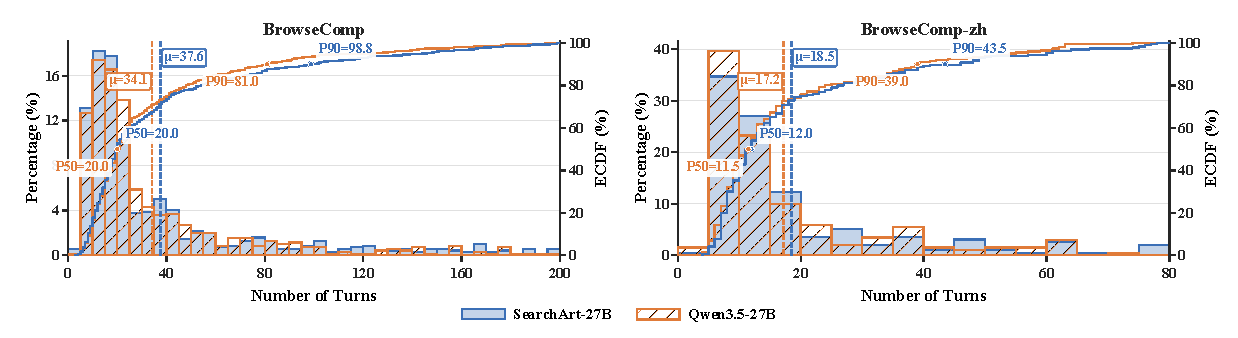
\includegraphics[width=1\linewidth]{img/any_correct_hist_ecdf_quantile_bg_noborder.pdf}
    \caption{Distributions of the number of turns on BrowseComp (left) and BrowseComp-zh (right). Bars show the percentage of trajectories, while solid curves represent the ECDFs. Annotations indicate the mean (\(\mu\)), 50th percentile (P50), and 90th percentile (P90).}
    \label{fig:post-train-behavior}
\end{figure}
\begin{figure}[!t]
    \centering
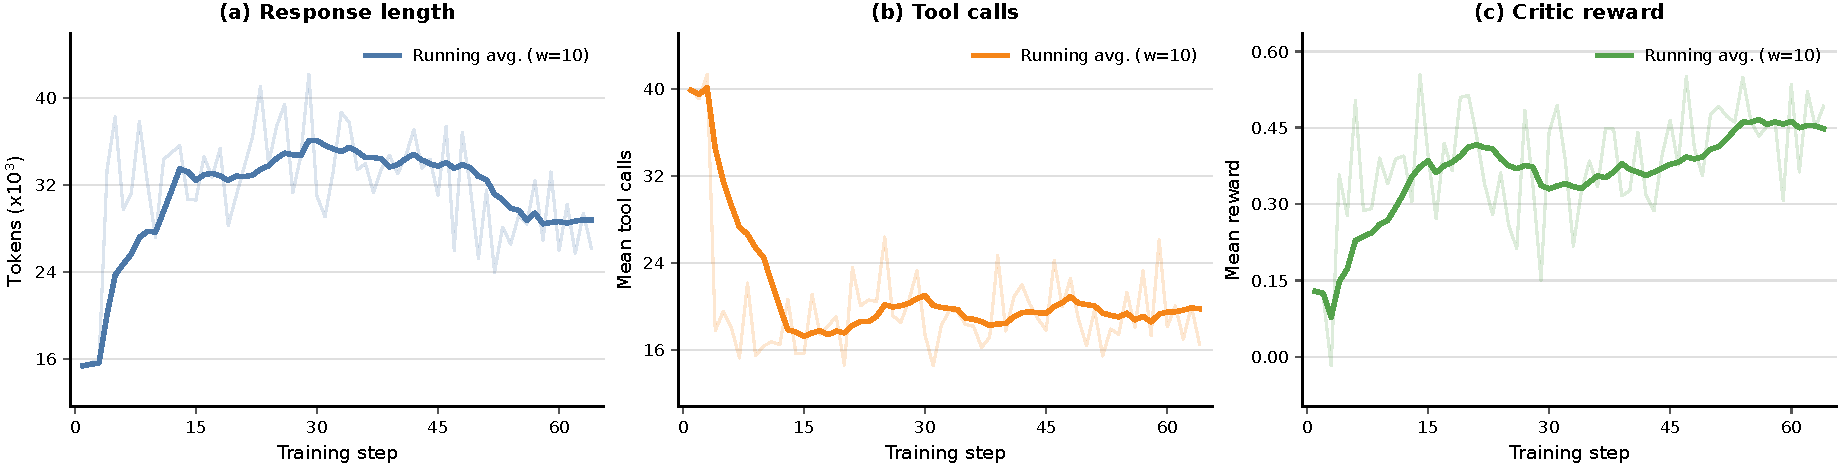
\includegraphics[width=1\linewidth]{img/training_curves_response_toolcalls_reward.pdf}
    \caption{Training dynamics of SearchArt-27B: (a) mean response length, (b) mean number of tool calls, and (c) mean critic reward.}
    \label{fig:post-train-process}
\end{figure}



Figure \redref{fig:post-train-behavior} highlights the more persistent search behavior of SearchArt-27B model. On both datasets, the ECDF of SearchArt-27B is generally shifted to the right of that of Qwen3.5-27B, indicating that SearchArt-27B is more willing to continue searching instead of terminating a trajectory prematurely. This difference is particularly pronounced on BrowseComp, where the mean turn count increases from 34.1 for Qwen3.5-27B to 37.6 for SearchArt-27B. Although both models have a median of 20 turns, the 90th percentile increases from 81.0 to 98.8 turns, showing that the additional search effort is concentrated primarily on difficult, long-running trajectories rather than being uniformly applied to all examples. A similar pattern is observed on BrowseComp-zh: SearchArt-27B has a mean of 18.5 turns compared with 17.2 for Qwen3.5-27B, while their 90th percentiles are 43.5 and 39.0 turns, respectively. These results suggest that fine-tuning enables SearchArt-27B to preserve a similar computational profile on typical cases while allocating a larger search budget to challenging instances. Such selective persistence is beneficial for agentic search tasks, where additional exploration can help gather more complete evidence and reduce the risk of premature termination.

\subsubsection{Training Process}
We show several key training dynamics in Figure \redref{fig:post-train-process}. The critic reward steadily improves throughout training, indicating that the policy learns to produce more successful trajectories. Meanwhile, the mean number of tool calls drops sharply during the early stage and subsequently stabilizes, suggesting that the agent learns a more efficient tool-use strategy. Response length initially increases as the model explores longer reasoning and tool-interaction trajectories, then gradually decreases and stabilizes, consistent with a transition toward more concise yet effective solutions.





\begin{figure}[!t]
    \centering
    \begin{subfigure}[t]{0.7\linewidth}
        \centering
        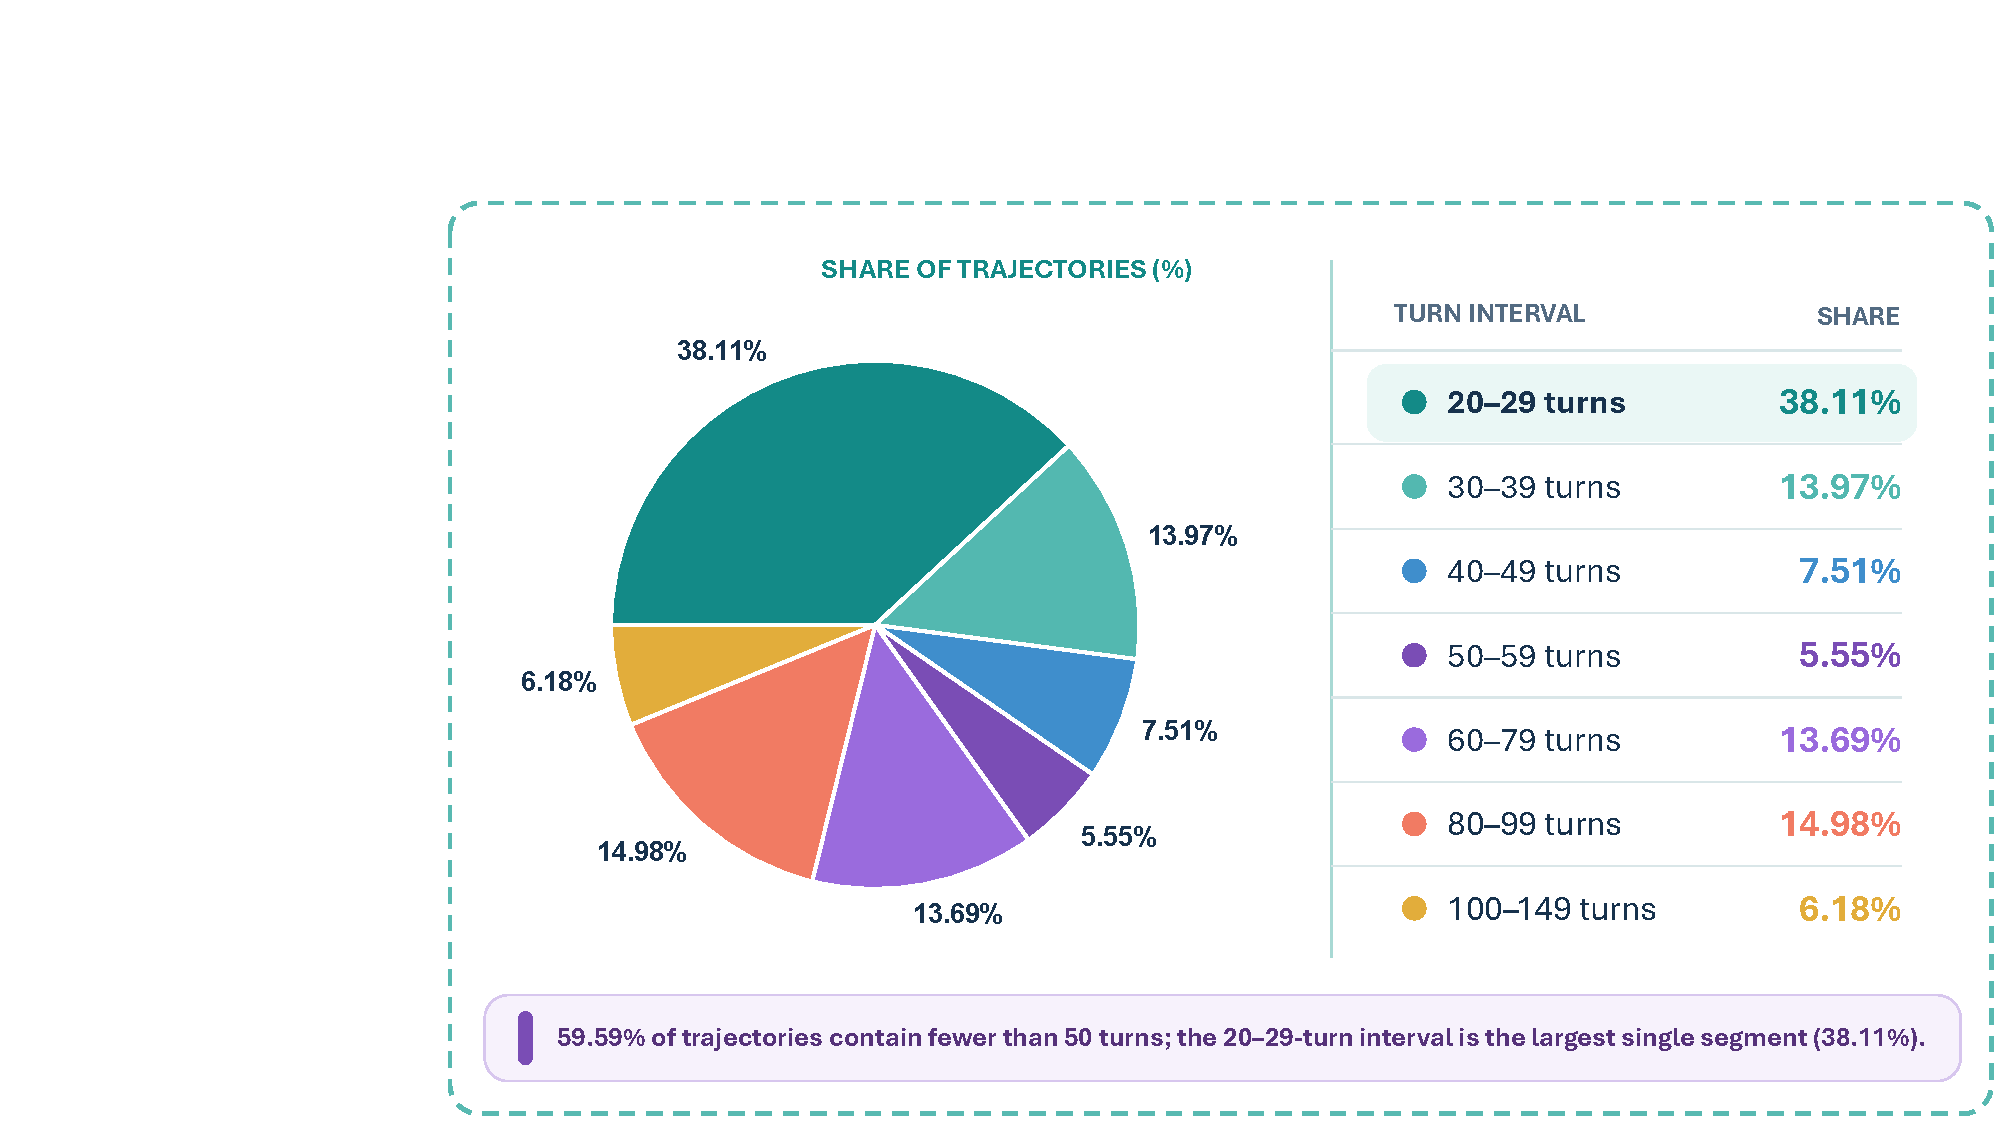
\includegraphics[width=\linewidth]{img/synthetic_qa_trajectory_distribution_v1.pdf}
        \caption{Trajectory turn distribution of DeepSearch QA.}
        \label{fig:synthetic_task_qa_trajectory_distribution_bright}
    \end{subfigure}
    \hfill
    \begin{subfigure}[t]{0.7\linewidth}
        \centering
        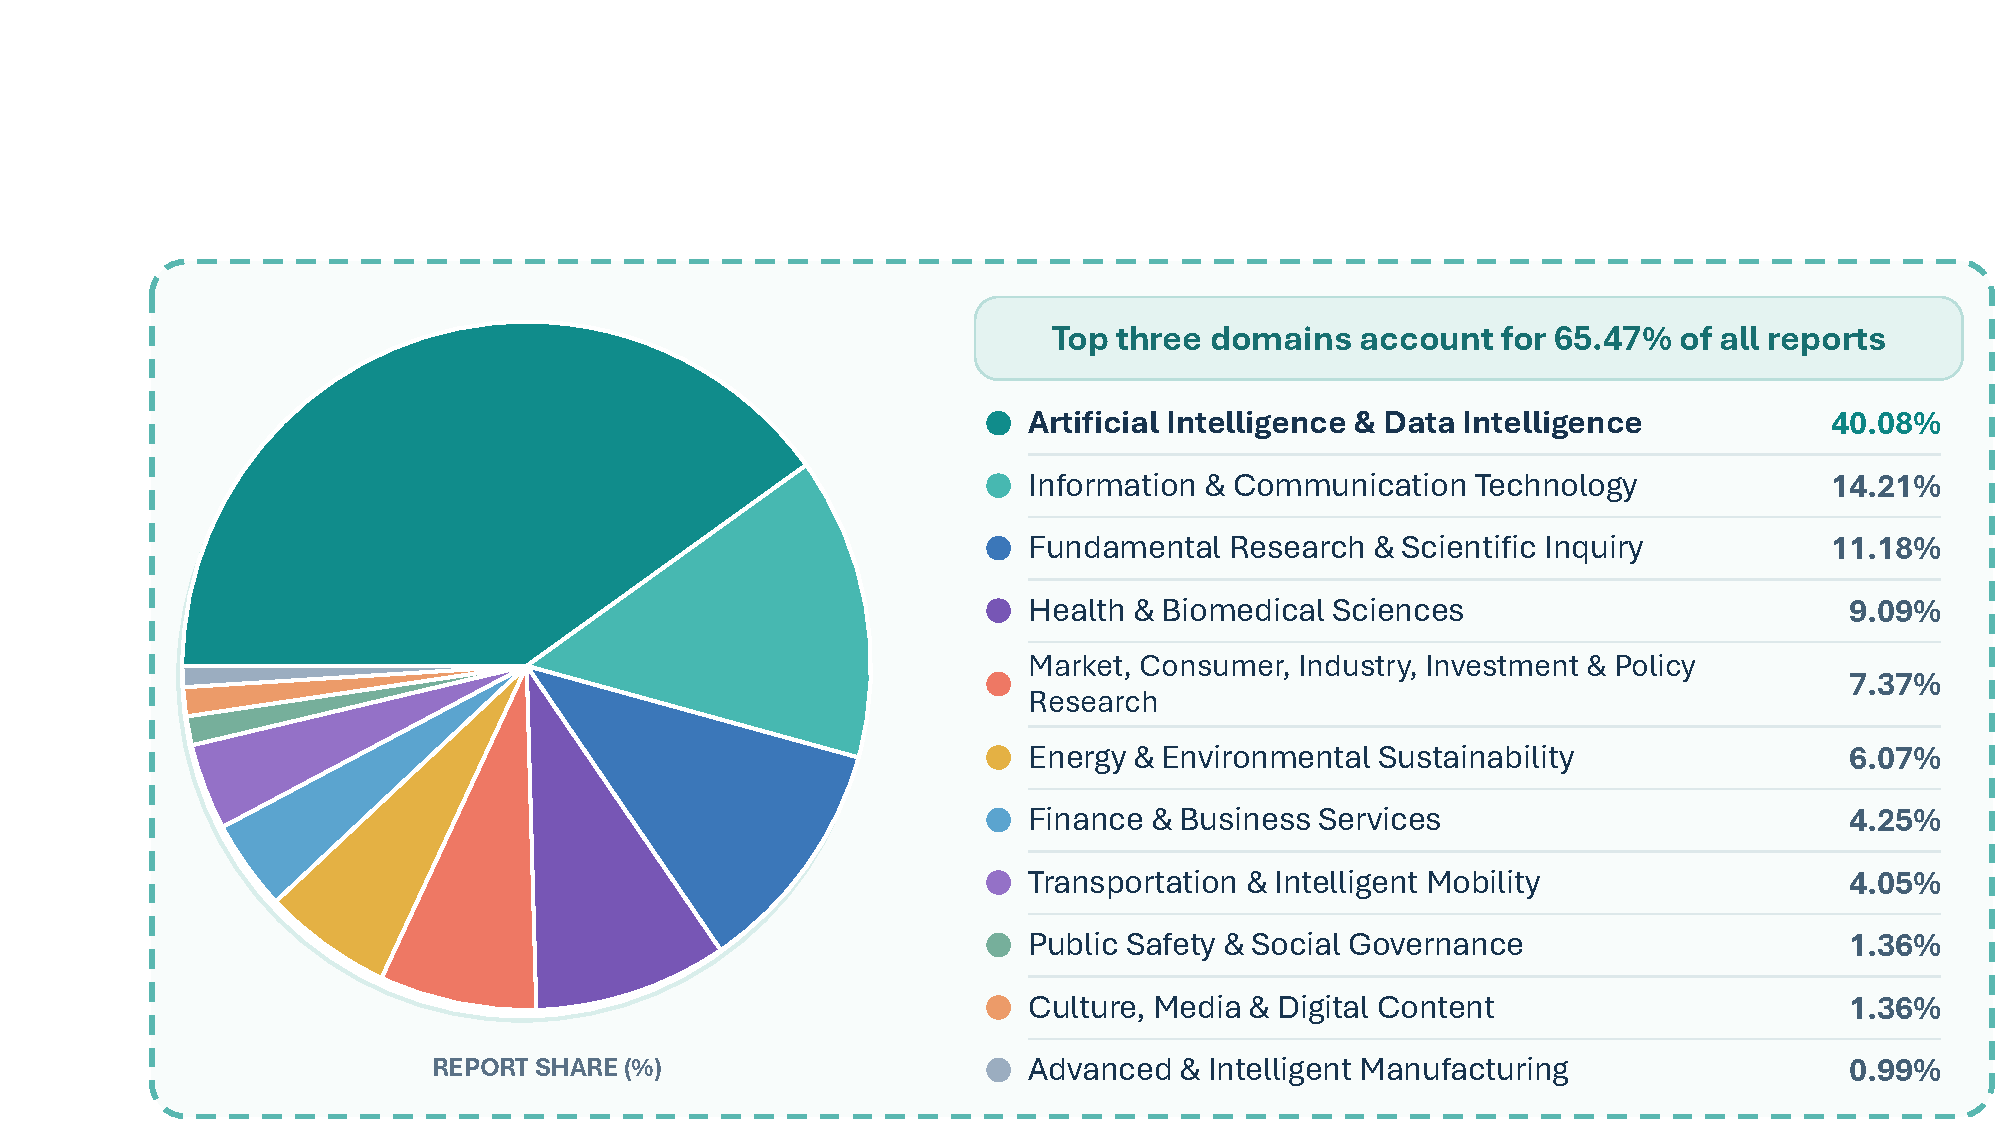
\includegraphics[width=\linewidth]
        {img/deepresearch-thematic-distribution_v1.pdf}
        \caption{Domain distribution of DeepResearch QA.}
        \label{fig:deepresearch_theme_distribution}
    \end{subfigure}

    \caption{Statistics of the synthesized QA datasets.}
    \label{fig:qa_synthesis_statistics}
\end{figure}


\subsubsection{Data Statistics}
Figure \redref{fig:qa_synthesis_statistics} summarizes the statistical distributions of the synthesized QA datasets. As shown in Figure \redref{fig:synthetic_task_qa_trajectory_distribution_bright}, DeepSearch QA contains search trajectories spanning from 20 to 149 interaction turns. The 20–29-turn interval constitutes the largest group, accounting for 38.11\% of all trajectories. Overall, 59.59\% of the trajectories contain fewer than 50 turns, while a substantial proportion involve considerably longer interactions: 19.24\% contain 50–79 turns, and 21.16\% contain at least 80 turns. This broad distribution indicates that DeepSearch QA covers search processes of varying lengths, including both relatively concise interactions and complex, long-horizon search trajectories.


Figure \redref{fig:deepresearch_theme_distribution} presents the domain distribution of DeepResearch QA. The dataset spans 11 domains, with Artificial Intelligence \& Data Intelligence representing the largest share at 40.08\%. It is followed by Information \& Communication Technology (14.21\%) and Fundamental Research \& Scientific Inquiry (11.18\%). Together, these three domains account for 65.47\% of all reports. The remaining examples cover a diverse range of areas, including health and biomedical sciences (9.09\%), market and policy research (7.37\%), energy and environmental sustainability (6.07\%), finance and business services (4.25\%), and transportation and intelligent mobility (4.05\%), as well as several smaller domains. Although the distribution emphasizes technology- and science-related topics, its broad domain coverage enables the evaluation of research agents across heterogeneous information needs.



\iffalse
\begin{table}[ht]%[htbp]
\scriptsize
\centering
\caption{Performance comparison of all methods on Wikipedia-based datasets. %$\dagger$ and $\star$  represent in-domain and out-domain datasets, respectively. 
We highlight the best performance among the trainable or frozen models in the same series.}
\begin{tabular}{l c c c c c c c c}
\toprule
\multirow{2}{*}{\textbf{Model}} & \multicolumn{3}{c}{\textbf{General QA}} & \multicolumn{4}{c}{\textbf{Multi-Hop QA}} &  \\
\addlinespace[0.1em]
\cline{2-8}
\addlinespace[0.3em]
 & \textbf{NQ} & \textbf{TriviaQA} & \textbf{PopQA} & \textbf{HotpotQA} & \textbf{2wiki} & \textbf{Musique} & \textbf{Bamboogle}$^{\star}$ & \textbf{Avg.} \\
\midrule
\multicolumn{9}{c}{\textbf{Non-decoupled Planner-Generator}} \\
\midrule
\multicolumn{9}{l}{\textbf{$\Rightarrow$ Qwen2.5-7b-Instruct}} \\
\addlinespace[0.1em]
\cdashline{1-9}
\addlinespace[0.3em]
\multicolumn{9}{l}{\textbf{$\downarrow$ Planner (Frozen) \& Generator (Frozen)}} \\
Direct Inference & 0.325 & 0.507 & 0.196 & 0.301 & 0.268 & 0.135 & 0.192 & 0.275 \\
Naive RAG & 0.585 & 0.753 & 0.489 & 0.478 & 0.325 & 0.162 & 0.408 & 0.457 \\
%Direct Inference (think) & 0.383 & 0.600 & 0.199 & 0.345 & 0.290 & 0.149 & 0.408 & 0.339(0.328) \\
%Direct Inference (nothink) & 0.325 & 0.507 & 0.196 & 0.301 & 0.268 & 0.135 & 0.192 & 0.275(0.289) \\
%Naive RAG (think) & 0.585 & 0.753 & 0.489 & 0.478 & 0.325 & 0.162 & 0.408 & 0.457(0.465) \\
%Naive RAG (nothink) & 0.586 & 0.757 & 0.508 & 0.525 & 0.380 & 0.228 & 0.392 & 0.482 \\
CoT & 0.370 & 0.583 & 0.178 & 0.299 & 0.278 & 0.109 & 0.432 & 0.321 \\
IRCoT & 0.537 & 0.703 & 0.442 & 0.394 & 0.194 & 0.105 & 0.336 & 0.387 \\
Search-o1 & 0.462 & 0.652 & 0.350 & 0.441 & 0.400 & 0.198 & 0.472 & 0.425 \\
\addlinespace[0.1em]
\cdashline{1-9}
\addlinespace[0.3em]
\multicolumn{9}{l}{\textbf{$\downarrow$ Planner (Trainable) \& Generator (Trainable)}} \\
SFT & 0.556 & 0.553 & 0.177 & 0.384 & 0.269 & 0.166 & 0.400 & 0.358 \\
%R1 &  &  &  &  &  &  &  &  \\
Search-R1 & \textbf{0.630} & \textbf{0.771} & 0.503 & 0.571 & 0.402 & 0.215 & 0.544 & 0.519 \\
%& 0.630 & 0.771 & 0.503 & 0.571 & 0.502 & 0.215 & 0.408 &  \\
\midrule
\multicolumn{9}{c}{\textbf{Generator Only (Frozen)}} \\
\midrule
\multicolumn{9}{l}{\textbf{$\Rightarrow$ Qwen3-32b}} \\
\addlinespace[0.1em]
\cdashline{1-9}
\addlinespace[0.3em]
Direct Inference & 0.486 & 0.737 & 0.276 & 0.451 & 0.364 & 0.218 & \textbf{0.648} & 0.454 \\
Naive RAG & 0.652 & \textbf{0.824} & 0.517 & 0.587 & 0.397 & 0.229 & 0.568 & 0.539 \\
%Direct Inference (think) & 0.486 & 0.737 & 0.276 & 0.451 & 0.364 & 0.218 & 0.648 & 0.454(0.422) \\
%Direct Inference (nothink) & 0.485 & 0.739 & 0.274 & 0.451 & 0.360 & 0.216 & 0.640 & 0.452(0.421) \\
%Naive RAG (think) & 0.652 & 0.824 & 0.517 & 0.587 & 0.397 & 0.229 & 0.568 & 0.539(0.534) \\
%Naive RAG (nothink) & 0.647 & 0.820 & 0.518 & 0.607 & 0.438 & 0.259 & 0.608 & 0.557(0.548) \\
\midrule
\multicolumn{9}{l}{\textbf{$\Rightarrow$ Deepseek-V3}} \\
\addlinespace[0.1em]
\cdashline{1-9}
\addlinespace[0.3em]
Direct Inference & 0.604 & \textbf{0.870} & 0.447 & 0.519 & 0.425 & 0.254 & 0.432 & 0.507 \\
Naive RAG & 0.670 & 0.840 & 0.527 & 0.606 & 0.438 & 0.241 & 0.424 & 0.535 \\
%Direct Inference (think) & 0.658 & 0.892 & 0.494 & 0.633 & 0.583 & 0.357 & 0.816 & 0.633 \\
%Direct Inference (nothink) & 0.604 & 0.870 & 0.447 & 0.519 & 0.425 & 0.254 & 0.432 & 0.507 \\
%Naive RAG (think) & 0.699 & 0.879 & 0.543 & 0.630 & 0.427 & 0.317 & 0.688 & 0.598 \\
%Naive RAG (nothink) & 0.670 & 0.840 & 0.527 & 0.606 & 0.438 & 0.241 & 0.424 & 0.535 \\
\midrule
\multicolumn{9}{l}{\textbf{$\Rightarrow$ Deepseek-R1}} \\
\addlinespace[0.1em]
\cdashline{1-9}
\addlinespace[0.3em]
Direct Inference & 0.657 & \textbf{0.903} & 0.499 & 0.655 & 0.594 & 0.365 & 0.632 & 0.615 \\
Naive RAG & 0.668 & \textbf{0.903} & 0.495 & 0.661 & 0.599 & 0.369 & 0.648 & 0.620 \\
%Direct Inference & 0.668 & 0.903 & 0.495 & 0.661 & 0.599 & 0.369 & 0.848 & 0.649 \\
%Naive RAG & 0.666 & 0.841 & 0.515 & 0.603 & 0.428 & 0.257 & 0.536 & 0.549 \\
\midrule
\multicolumn{9}{c}{\textbf{Decoupled Planner-Generator}} \\
\midrule
\multicolumn{9}{l}{\textbf{$\Rightarrow$ AI-SearchPlanner}} \\
\addlinespace[0.1em]
\cdashline{1-9}
\addlinespace[0.3em]
\multicolumn{9}{l}{$\downarrow$ \textbf{Planner (Trainable)}: Qwen2.5-7b-Instruct \textbf{\&} \textbf{Generator (Frozen)}: Qwen3-32b} \\
\multicolumn{1}{c}{$\alpha$ = 0}  & \textbf{0.674} & 0.800 & \textbf{0.540} & \textbf{0.678} & \textbf{0.565} & \textbf{0.355} & 0.568 & \textbf{0.597}(+10.76\%) \\
\multicolumn{9}{l}{\textbf{Generator Transferability}} \\
Qwen2.5-7b-Instruct & 0.628 & 0.764 & \textbf{0.517} & \textbf{0.638} & \textbf{0.462} & \textbf{0.320} & \textbf{0.552} & \textbf{0.554}(+6.74\%) \\
Deepseek-V3 & \textbf{0.678} & 0.833 & \textbf{0.534} & \textbf{0.671} & \textbf{0.562} & \textbf{0.349} & \textbf{0.640} & \textbf{0.610}(+14.02\%) \\
Deepseek-R1 & \textbf{0.719} & 0.880 & \textbf{0.549} & \textbf{0.741} & \textbf{0.617} & \textbf{0.373} & \textbf{0.656} & \textbf{0.648}(+4.52\%) \\
%\addlinespace[0.1em]
%\cdashline{1-9}
%\addlinespace[0.3em]
%\multicolumn{9}{l}{$\downarrow$ \textbf{Planner (Frozen)}: Qwen2.5-7b-Instruct} \\
%\multicolumn{9}{l}{\textbf{Generator (Frozen)}} \\
%Qwen3-32b & 0.616 & 0.772 & 0.447 & 0.623 & 0.528 & 0.325 & 0.520 & 0.547 \\
%Qwen2.5-7b-Instruct & 0.563 & 0.722 & 0.385 & 0.581 & \textbf{0.492} & 0.281 & 0.520 & 0.506 \\
%Deepseek-V3 & 0.651 & 0.837 & 0.447 & 0.641 & 0.524 & 0.305 & 0.637 & 0.577 \\
%Deepseek-R1 & & & & & & & & \\
%w/ Qwen3-32b & 0.655 & 0.793 & 0.490 & 0.526 & 0.602 & 0.300 & 0.544 & 0.559 \\
%w/ Qwen3-32b & 0.653 & 0.791 & 0.499 & 0.607 & 0.530 & 0.293 & 0.536 & 0.558 \\
%w/ Qwen3-32b & 0.701 & 0.806 & 0.567 & 0.678 & 0.605 & 0.321 & 0.604 & 0.612 \\
\bottomrule
\end{tabular}
\vspace{-0.5cm}  % 减少下方空白
\label{tab:wiki_dataset}
\end{table}
\fi



\section{Related Work}
\subsection{Agentic Large Language Models}
A growing body of research on LLMs \cite{naveed2025comprehensive, zhao2023survey, achiam2023gpt, qwenbai2023qwen, liu2024deepseek, guo2025deepseek, xu2026deepseek, yin2024survey} has shifted toward the development of agentic systems \cite{singh2025agentic, wu2025agentic, wu2025agentic1}. Such systems are designed to transform high-level objectives into sequences of manageable actions, select and operate external tools, and revise their plans in response to observations obtained during execution. 
In contrast to traditional conversational models \cite{lewis2020retrieval, gao2023retrieval, mei2025survey, liu2025llm4ranking, gong2026cardrewriter, niu2025distributionally, mei2025dense, niu2025addressing, mei2023improving}, which typically generate an answer within a single interaction step, agentic LLMs \cite{openai2026, anthropic2026, google2026, xu2026deepseek, qwen2026, zeng2026glm, MiniMaxAI2026, seed2026seed2, kimi2026} operate through multi-step decision processes and maintain contextual state throughout an extended workflow.


These abilities are now being incorporated into state-of-the-art models through both training-time optimization and specialized inference-time architectures. Notable examples include GPT-5.5 \cite{openai2026}, Claude-4.8 \cite{anthropic2026}, Gemini-3.1 Pro \cite{google2026}, DeepSeek-V4 \cite{xu2026deepseek}, Qwen3.5-397B \cite{qwen2026}, GLM-5.1 \cite{zeng2026glm}, Minimax-M2.5 \cite{MiniMaxAI2026}, Seed-2.0-Pro \cite{seed2026seed2}, and Kimi-K2.6 \cite{kimi2026}. Across tasks involving complex reasoning, software development, and multimodal understanding, these models exhibit increasingly competitive capabilities. Many of them also provide support for large context windows, structured tool use, and the execution of multi-step operations.


Collectively, these advances reflect a broader transition in the role of foundation models. Rather than functioning solely as systems for language generation, modern LLMs are increasingly positioned as general-purpose agents that can plan, act, adapt, and interact with external environments to complete complex tasks.



\subsection{Deep Search \& Research Agents}
The rapid development of agentic LLMs \cite{openai2026, anthropic2026, google2026, xu2026deepseek, qwen2026, zeng2026glm, MiniMaxAI2026, seed2026seed2, kimi2026} has given rise to a new category of systems commonly referred to as deep search \& research agents. These systems target open-ended research and knowledge-synthesis tasks that require extensive information retrieval, sustained reasoning, and the integration of evidence across heterogeneous sources. In contrast to conventional language models \cite{lewis2020retrieval, gao2023retrieval, mei2025survey, liu2025llm4ranking, gong2026cardrewriter, niu2025distributionally, mei2025dense, niu2025addressing, mei2023improving} that primarily generate responses from parametric knowledge, deep research agents continuously interact with external information environments. They formulate search strategies, gather relevant materials, revise intermediate assumptions, identify unresolved knowledge gaps, and consolidate the collected evidence into structured research reports.


A number of commercial systems have demonstrated the practical potential of this paradigm. Prominent examples include OpenAI Deep Research \cite{openai2026}, Claude Research \cite{anthropic2026}, Kimi-Researcher \cite{kimi2026}, and Gemini Deep Research \cite{google2026}. Although their implementations differ, these systems generally combine foundation models with web access, iterative planning, retrieval, and evidence synthesis to support relatively autonomous research workflows. OpenAI Deep Research, for example, integrates a reasoning model with multi-stage web exploration and asynchronous task execution. Gemini Deep Research constructs adaptive research plans that can be refined during interaction, while benefiting from the self-reflective reasoning and long-context capabilities of Gemini models. Claude Research follows an agentic search process in which successive retrieval steps build upon previous findings and explore a question from multiple perspectives. Perplexity Deep Research similarly combines large-scale search infrastructure with lexical and semantic retrieval mechanisms to identify and rerank relevant information.


Alongside industrial systems, the research community has proposed a growing number of open models and frameworks for deep research. Representative efforts include MiroThinker \cite{team2026mirothinker}, WebThinker \cite{li2026webthinker}, Tongyi-DeepResearch \cite{team2025tongyi}, OpenSeeker \cite{du2026openseeker}, REDSearcher \cite{chu2026redsearcher}, and Step-DeepResearch \cite{hu2025step}. These studies investigate different mechanisms for extending the research horizon of language-model agents, including iterative search, explicit planning, self-reflection, trajectory learning, and evidence-grounded synthesis. In particular, agent-oriented mid-training has become an increasingly common approach for improving the ability of models to interact with tools and execute long sequences of research actions. Systems such as Tongyi DeepResearch, REDSearcher, and Step-DeepResearch employ this strategy to internalize agentic behaviors rather than relying exclusively on inference-time prompting and external control logic.

Despite their effectiveness, most existing deep research systems continue to rely on general-purpose foundation models whose research capabilities are largely induced through externally designed workflows. Planning procedures, retrieval loops, reflection stages, and report-generation patterns are often explicitly encoded in the system architecture. Such designs can provide reliable behavioral structure, but they also introduce considerable engineering complexity and may limit the agent's ability to adapt beyond predefined execution patterns. Moreover, lightweight prompting-based agents, including many standard ReAct implementations, often perform only shallow exploration in specialized or technically demanding domains. They may terminate retrieval prematurely, overlook important evidence, or fail to develop sufficiently detailed analyses to satisfy users' actual research needs. These limitations motivate the development of research agents that can acquire stronger long-horizon search and reasoning capabilities at the model level while retaining flexibility across diverse research scenarios.

\iffalse
\subsection{Optimization of Research Capabilities}
Unlike orchestration-based systems, some works internalize relevant capabilities into models through end-to-end training. DeepResearcher conducts end-to-end RL training via GRPO in real web environments, demonstrating emergent cognitive behaviors such as planning, cross-source verification, and self-reflection. Kimi-Researcher supports long-horizon multi-turn search reasoning through end-to-end agentic RL training, employing context management mechanisms and asynchronous rollout systems. Tongyi DeepResearch proposes a unified training paradigm for agentic mid-training and post-training, combining automated data synthesis pipelines with on-policy RL. Related agent training methodology works such as WebRL, which proposes autonomous curriculum learning and KL-constrained policy updates, and Search-R1, which adopts RL-enhanced search reasoning integration, have made progress in this area.
Nevertheless, existing end-to-end works still primarily focus on improving “search efficacy” (e.g., retrieval accuracy, query optimization), lacking systematic construction strategies for “atomic core capabilities” crucial to in-depth research, such as long-horizon logical reasoning, multi-source cross-validation, and high-quality report composition.
Furthermore, how to optimize model size and inference cost while maintaining high performance remains an urgent challenge for the industry.

\subsection{Deep Research Related Evaluation Benchmarks}
In terms of evaluation, ResearchRubrics contains 101 domain-diverse research tasks, each equipped with 20-43 expert-written fine-grained scoring criteria, assessing factual accuracy, reasoning soundness, and clarity. DeepResearch Bench comprises 100 PhD-level research tasks spanning 22 domains, evaluating report quality through the RACE framework and information retrieval capabilities through the FACT framework. ReportBench reverse-engineers research questions based on expert survey papers on arXiv, assessing the citation accuracy and factual consistency of generated reports. However, these academic datasets for Deep Research, except for ResearchRubrics, remain insufficient in terms of task coverage comprehensiveness and evaluation depth, failing to adequately cover the diverse requirements of real research scenarios.
Another category of benchmarks focuses more on retrieval and knowledge testing capabilities. BrowseComp contains 1,266 fact-finding questions requiring multi-hop reasoning, directly targeting the evaluation of models’ ability to retrieve deeply hidden information. HLE (Humanity’s Last Exam) includes 2,500 expert-level questions across multiple disciplines, yet still carries a strong “closed-book exam” flavor, largely focusing on multi-hop search with definitive answers or frontier knowledge testing, failing to fully reach the openness and multidimensionality of real industrial-grade research scenarios. To this end, we construct ADR-Bench, aiming to fill the evaluation gap for Chinese Deep Research scenarios driven by real user demands.


\subsection{Data synthesis for deep research agents}
High-quality synthetic data is the key to the agentic search capabilities. Current approaches to agentic data synthesis mainly follow two paradigms: (1) graph-based methods traverse knowledge graphs to synthetic multi-hop QA data; (2) agent-based methods use agents explore real web environments for data synthesis. Despite their differences, both paradigms face a common and fundamental challenge: automatically synthesizing difficult QA pairs with unique and correct answers. To address this issue, we design a verification-driven method to improve QA data quality.



\subsection{Trajectory construction}
The ReAct paradigm serves as the foundation of most current agentic systems. Recent works have improved upon ReAct through procedural planning, multi-agent orchestration, and context management. However, these frameworks share a critical limitation: the absence of explicit verification during interactions. In long-horizon information seeking, agents must navigate massive search spaces where intermediate results are often noisy or misleading. Without a dedicated verification mechanism, agents are prone to accepting the first plausible-looking answer and terminating exploration prematurely, even when the result is incorrect. To address this limitation, we introduce an explicit verification mechanisms for both intermediate search results and final answers, designed to effectively teach the model robust verification behaviors.



\subsection{Context Management for Agents}
Managing growing context has attracted considerable recent attention, with existing methods falling into four categories. Sliding-window heuristics such as keep-last-k—adopted by the MiroThinker series—retain only recent steps and discard older content regardless of importance, while discard-all variants flush the entire context once thresholds are reached, as in DeepSeek-V3.2 and GLM-4.7. Periodic summarization methods such as MEM1 train agents to maintain compact internal states and achieve strong multi-hop QA performance, while MemAgent processes documents in segments with fixed-size memory buffers. Proactive curation approaches such as AgentFold and ARC enable agents to actively decide what and when to compress, yet they still lack surgical operations and cannot revisit earlier history to purge outdated content.

\fi



\section{Conclusion}
In this technical report, we presented \textbf{SearchArt}, a scalable framework for developing long-horizon search agents through verification-driven synthetic task generation and multi-stage post-training. SearchArt addresses several central challenges in search-agent training, including the limited availability of high-quality QA pairs, the high cost of manually annotated interaction trajectories, and the difficulty of providing reliable supervision for intermediate retrieval and reasoning behaviors. By constructing complex multi-hop information-seeking tasks from web documents and automatically generated evidence graphs, the framework produces both diverse QA pairs and corresponding long-horizon search trajectories at scale.


A key component of SearchArt is its verification pipeline, which jointly examines QA consistency, trajectory reliability, and the relevance of retrieved evidence. This process filters out shallow, redundant, or weakly grounded training examples and provides more reliable supervision for learning effective search policies. The verified trajectories are subsequently incorporated into a multi-stage post-training pipeline consisting of supervised fine-tuning and reinforcement learning-based policy optimization. Rather than optimizing only for final-answer correctness, SearchArt explicitly improves intermediate behaviors such as query formulation, evidence-branch selection, iterative information aggregation, search-budget allocation, and the timing of answer generation.


Experiments based on the Qwen3.5 model series across open-domain deep-search and deep-research benchmarks demonstrate that SearchArt substantially improves task-completion accuracy over the corresponding base models and search agents of comparable scale. The resulting agents exhibit stronger adaptive planning, more sustained evidence exploration, and more reliable reasoning over extended interaction horizons. These results indicate that the quality and structure of synthetic supervision are as important as its scale, particularly for tasks that require repeated retrieval, cross-source evidence integration, and long-horizon decision making.


Overall, SearchArt demonstrates that verification-driven synthetic task construction, combined with trajectory-level supervised and reinforcement learning, provides a practical and scalable approach to training capable search agents. By jointly improving task diversity, trajectory quality, and intermediate behavioral supervision, the framework offers a systematic foundation for building search and research agents that operate more effectively and reliably in complex, open-ended information environments.


\section{Future Work}

Building on the current SearchArt framework, we identify two primary directions for extending search agents toward more general and research-capable autonomous systems. The first direction concerns the transition from text-centric search to multimodal information seeking, while the second aims to develop an automated research framework capable of producing rigorous, evidence-grounded, and publication-style research reports.

\paragraph{Multimodal Search Agents.}
The current framework primarily focuses on textual information retrieval and reasoning. However, many real-world information environments contain heterogeneous modalities, including images, figures, tables, charts, slide decks, videos, and visually structured documents. Extending SearchArt to multimodal settings therefore requires agents that can not only retrieve information across different media formats, but also determine which modality is most informative at each stage of the search process. A multimodal search agent should be able to formulate modality-aware queries, interpret visual and textual evidence jointly, and establish correspondences between claims expressed in different representational forms. For example, the agent may need to connect a textual description with evidence contained in a scientific figure, compare numerical results across tables, or integrate information extracted from webpages, PDFs, images, and videos.


This extension also introduces new challenges for data construction, verification, and post-training. Multimodal synthetic tasks must capture cross-modal dependencies that cannot be resolved through textual evidence alone, while the corresponding trajectories should reflect modality selection, visual grounding, cross-modal evidence alignment, and iterative refinement of retrieval strategies. Verification mechanisms must further evaluate whether visual evidence genuinely supports the generated answer and whether the agent has correctly interpreted the relevant regions, objects, relations, or numerical values. By incorporating these signals into supervised fine-tuning and reinforcement learning, SearchArt can be extended from an NLP-oriented search framework into a general multimodal search-agent training system capable of operating over richer and more realistic information environments.

\paragraph{AutoResearch.}
A second direction is to advance search agents from complex information retrieval toward end-to-end automated research. Compared with conventional search tasks, scientific research requires substantially more than locating and aggregating relevant information. An AutoResearch system must formulate research questions, decompose them into verifiable subproblems, collect and organize evidence, compare competing explanations, identify limitations, and produce a coherent research report that satisfies domain-specific standards of rigor. Developing such a system requires the joint design of scalable research-task synthesis, fine-grained evaluation rubrics, research-oriented post-training objectives, and a structured inference harness for long-running research workflows.


At the data level, synthetic research tasks should cover diverse scientific domains and include explicit supervision for research planning, literature analysis, evidence comparison, hypothesis development, methodological reasoning, and report organization. At the evaluation level, rubrics should assess not only factual correctness, but also coverage, novelty, methodological validity, evidential sufficiency, citation quality, logical coherence, and the consistency between claims and supporting sources. These rubric-based signals can subsequently guide supervised fine-tuning and reinforcement learning, enabling the model to optimize intermediate research behaviors rather than merely the final report. In parallel, the inference harness should support hierarchical planning, persistent evidence management, context compression, iterative verification, citation tracking, and modular report generation. Integrating data synthesis, rubric-based evaluation, post-training, and harness-level orchestration would allow SearchArt to evolve into an AutoResearch framework capable of generating research-grade, well-structured, and evidence-grounded scientific reports through extended autonomous interaction.





\begingroup
\renewcommand{\thefootnote}{\fnsymbol{footnote}}
\setcounter{footnote}{0}

\section{Contributions}
\paragraph{Cores:} Lang Mei, Xiaohan Yu, Chong Chen\footnote{Team Leader}, Liyan Liu, Xiangnan Chen, Jinchao Ma, Chao Feng, Li Huang, Siyu Mo, Sichen Kang, Yunkun Xu, Zhihan Yang, Zhujun Xue, Jingren Zhang

\paragraph{Contributors (in alphabetical order by surname initial):} Qing He, Yingdi Huang, Hao Jiang, Ziao Ma, Zewei Pan, Minhao Sun, Zhuo Tao, Jinzhao Xiao, Gangtao Xin, Huanyao Zhang, Wenjian Zhang, Jiangshan Zhang, Guojie Zhu


\paragraph{Academic Contributors (in alphabetical order by surname initial):} Jiaxin Mao (Renmin University of China), Wentao Zhang (Peking University). 

\endgroup



%\section*{References}


\bibliographystyle{plainnat}
\bibliography{ref}


%%%%%%%%%%%%%%%%%%%%%%%%%%%%%%%%%%%%%%%%%%%%%%%%%%%%%%%%%%%%
\newpage
\appendix


\section{Case}

\subsection{DeepSearch QA}
\label{appendix:DeepSearch QA}
\begin{tcolorbox}[
    title={English Example (125-turn tool use with Qwen3.7-Max)},
    colback=gray!5,
    colframe=gray!40,
    fonttitle=\bfseries,
    boxrule=0.5pt,
    arc=2pt,
    breakable
]
\ttfamily
\textbf{Question:} The British telegraph director who narrowly escaped drowning in the Red Sea when his ship wrecked in the late 1860s hired a Thuringian-born engineer who famously documented a Middle Eastern city using a plate camera. This Thuringian engineer married an Armenian woman whose father served as a general for a prominent royal figure. This royal figure sent the very first domestic telegram in his country to his brother. What specific city was this brother located in when he received this historic message?

\textbf{Golden Answer:} Shiraz 
\end{tcolorbox}

\begin{tcolorbox}[
    title={Chinese Example (104-turn tool use with Qwen3.7-Max)},
    colback=gray!5,
    colframe=gray!40,
    fonttitle=\bfseries,
    boxrule=0.5pt,
    arc=2pt,
    breakable
]
\ttfamily
\textbf{Question:} 在2024年秋季于科罗拉多州北部一所州立大学年度试验花园进行的一项研究中，某一种特定颜色的花朵每1000张图像的标准化访花率为26.06次。一位英国昆虫学家极力推荐种植一种常开此类颜色花朵的本土野花（其基原物种的花冠内面近基部具有斜向毛环，且有时呈污白色），同时建议避免种植蜀葵等重瓣花。请问，这位昆虫学家是在他的哪本著作中提出人类可以通过将土地转变为小型自然保留区来与自然健康共存的？


\textbf{Golden Answer:} 《寂静的地球》
\end{tcolorbox}



\subsection{DeepResearch QA}
\label{appendix:DeepResearch QA}
\begin{tcolorbox}[
    title={English Example},
    colback=gray!5,
    colframe=gray!40,
    fonttitle=\bfseries,
    boxrule=0.5pt,
    arc=2pt,
    breakable
]
\ttfamily
\textbf{Question:} What are the current research approaches and methodologies that integrate communication and computation in wireless networks, particularly focusing on how interference can be leveraged for distributed computation rather than treating these as separate optimization problems?
\end{tcolorbox}

\begin{tcolorbox}[
    title={Chinese Example},
    colback=gray!5,
    colframe=gray!40,
    fonttitle=\bfseries,
    boxrule=0.5pt,
    arc=2pt,
    breakable
]
\ttfamily
\textbf{Question:} 请深度调研2024年中国家电行业基础云应用的现状、趋势与挑战，包括家电企业上云的主要驱动因素、用云场景、云服务选型偏好（尤其是安全合规、成本控制、出海需求等方面），以及基础云如何支撑家电企业的数字化转型、智能家居业务和大模型应用

\end{tcolorbox}



\subsection{Real-world User Experience–oriented QA}
\label{appendix:Real-world User Experience–oriented QA}
\begin{tcolorbox}[
    title={Example},
    colback=gray!5,
    colframe=gray!40,
    fonttitle=\bfseries,
    boxrule=0.5pt,
    arc=2pt,
    breakable
]
\ttfamily
\textbf{Question:} 2025-2026雪季，崇礼哪些雪场更适合新手？请从初级道、教练、交通、价格和人多不多几个方面比较。\\

\textbf{Question:} 截至2026年5月22日，张艺谋、冯小刚、姜文自2000年以来分别执导过哪些电影？请整理每部电影的豆瓣评分、中国内地票房和主要获奖情况，并分析三位导演这些作品市场表现和口碑差异的成因。\\

\textbf{Question:} 截至2026年5月，面向个人用户的国产 AI 编程工具或 coding plan 有哪些？请整理主要厂商的价格、套餐、token或调用额度、额度刷新规则、可用模型、公开性能或用户反馈；如果TTFT、TPS等指标没有公开资料，请标注缺失。最后按性价比推荐一个最适合个人订阅的方案，并用Markdown格式输出。\\

\textbf{Question:} 截至2026年5月，帮我整理美剧《紧急呼救》（9-1-1）已播各季中出现过的主要插曲歌单，按季列出歌曲名和歌手。
\end{tcolorbox}




\subsection{DeepResearch Outline}
\label{appendix:DeepResearch Outline}
\begin{tcolorbox}[
    title={Example of Hierarchical Research Outline},
    colback=gray!5,
    colframe=gray!40,
    fonttitle=\bfseries,
    boxrule=0.5pt,
    arc=2pt,
    breakable
]
\ttfamily
\textbf{Question:} What are the trends in China’s computing power market?

\textbf{Outline:} 

\textcolor{TitleRed}{1. Overview of China’s Computing Power Market}

\textcolor{TitleRed}{1.1 Market Size and Growth [citation]1, 2, 3, 4, 9, 18[/citation]}

\textcolor{TitleRed}{1.1.1 Total Computing Power Capacity}
\begin{itemize}[leftmargin=1em, listparindent=\parindent]
\item China’s total computing power capacity reached 280 EFLOPS in 2024. [citation]1, 4[/citation]
\item It is expected to exceed 300 EFLOPS in 2025 and 2,500 EFLOPS by 2030. [citation]2, 9[/citation]
\item China’s computing power capacity has recorded an average annual growth rate of 48\% over the past eight years. [citation]22[/citation]
\end{itemize}


\textcolor{TitleRed}{1.1.2 Intelligent Computing Power Capacity}
\begin{itemize}[leftmargin=1em, listparindent=\parindent]
\item Intelligent computing power capacity reached 725.3 EFLOPS in 2024, representing year-on-year growth of 74.1\%. [citation]1, 14[/citation]
\item It is expected to reach 1,037.3 EFLOPS in 2025, an increase of 43\%. [citation]1, 3[/citation]
\item It is projected to reach 2,781.9 EFLOPS by 2028, with a CAGR of 46.2\% from 2023 to 2028. [citation]3[/citation]
\end{itemize}

\textcolor{TitleRed}{1.1.3 General-Purpose Computing Power Capacity}
\begin{itemize}[leftmargin=1em, listparindent=\parindent]
\item General-purpose computing power capacity reached 71.5 EFLOPS in 2024, up 20.6\% year on year. [citation]1[/citation]
\item It is expected to reach 85.8 EFLOPS in 2025, representing growth of 20\%. [citation]1[/citation]
\item The CAGR from 2023 to 2028 is projected to be 18.8\%. [citation]1, 3[/citation]
\end{itemize}

\textcolor{TitleRed}{1.1.4 Market Size by Value}
\begin{itemize}[leftmargin=1em, listparindent=\parindent]
\item China’s computing power market is expected to reach RMB 835.1 billion in 2025, representing year-on-year growth of more than 30\%. [citation]2, 4[/citation]
\item The market is projected to reach RMB 1.05 trillion in 2026 and nearly RMB 2 trillion by 2030. [citation]2, 4[/citation]
\item The AI server market is expected to reach RMB 296.346 billion in 2025, accounting for 67.01\% of the computing server market. [citation]18[/citation]
\end{itemize}


\textcolor{TitleRed}{1.2 Global Competitiveness and Ranking [citation]16, 22[/citation]}

\textcolor{TitleRed}{1.2.1 Global Computing Power Ranking}
\begin{itemize}[leftmargin=1em, listparindent=\parindent]
\item China ranks second globally in computing power, with a score of 70, behind only the United States, which scores 77. [citation]16[/citation]
\item China and the United States are both classified as “front-runners,” with China recording the largest improvement worldwide. [citation]16[/citation]
\end{itemize}

\textcolor{TitleRed}{1.2.2 Global Position in Intelligent Computing Power}
\begin{itemize}[leftmargin=1em, listparindent=\parindent]
\item By the end of 2025, China’s intelligent computing power capacity is expected to reach 1.59 million PFLOPS, ranking second globally. [citation]16, 22[/citation]
\item China has built 42 intelligent computing clusters containing at least 10,000 accelerator cards each, while its operational computing facilities contain more than 13.73 million standard racks. [citation]16, 22[/citation]
\end{itemize}


\textcolor{TitleRed}{2. Structural Characteristics of the Computing Power Market}

\textcolor{TitleRed}{2.1 Computing Power Mix [citation]1, 3, 13[/citation]}

\textcolor{TitleRed}{2.1.1 Shares of Training and Inference Computing}
\begin{itemize}[leftmargin=1em, listparindent=\parindent]
\item In 2023, training workloads accounted for 58.7\% of computing power demand, while inference workloads accounted for 41.3\%. [citation]13[/citation]
\item The share of inference demand is expected to reach 72.6\% in 2027 and 73.0\% in 2028. [citation]13[/citation]
\item Demand for inference computing has significantly greater growth potential than training computing and is expected to become the primary source of future growth. [citation]13[/citation]
\end{itemize}

\textcolor{TitleRed}{2.1.2 Intelligent and General-Purpose Computing Mix}
\begin{itemize}[leftmargin=1em, listparindent=\parindent]
\item In 2024, intelligent computing accounted for 32\% of total computing power, while general-purpose computing accounted for 68\%. [citation]5[/citation]
\item The growth rate of intelligent computing power, at 74.1\%, significantly exceeded the 20.6\% growth rate of general-purpose computing power. [citation]1[/citation]
\end{itemize}

\textcolor{TitleRed}{2.2 Industry Chain Structure [citation]4, 12, 15[/citation]}

\textcolor{TitleRed}{2.2.1 Upstream: Core Hardware and Equipment}
\begin{itemize}[leftmargin=1em, listparindent=\parindent]
\item AI chips: Cambricon, Huawei Ascend, Baidu Kunlun, and Hygon Information Technology. [citation]12, 15[/citation]
\item Servers: Inspur Information, Sugon, H3C, and Nettrix. [citation]12, 15, 18[/citation]
\item Storage equipment: Yangtze Memory Technologies Co. [citation]15[/citation]
\item Network equipment: Innolight Technology and Ruijie Networks. [citation]15[/citation]
\end{itemize}

\textcolor{TitleRed}{2.2.2 Midstream: Data Centres and Computing Services}
\begin{itemize}[leftmargin=1em, listparindent=\parindent]
\item Data centre operators: VNET Group and Range Intelligent Computing Technology. [citation]15[/citation]
\item Cloud computing services: China Telecom Cloud, Alibaba Cloud, Tencent Cloud, and Huawei Cloud. [citation]12, 15[/citation]
\item Computing power scheduling: Sugon and China Telecom. [citation]15[/citation]
\end{itemize}

\textcolor{TitleRed}{2.2.3 Downstream: Industry Applications}
\begin{itemize}[leftmargin=1em, listparindent=\parindent]
\item In the internet sector, general-purpose computing accounts for 39\%, while intelligent computing accounts for 53\%. [citation]7[/citation]
\item Other major application sectors include finance, manufacturing, telecommunications, government, healthcare, and education. [citation]7, 15[/citation]
\end{itemize}

\textcolor{TitleRed}{2.3 Regional Distribution [citation]6, 11, 15[/citation]}

\textcolor{TitleRed}{2.3.1 Layout of National Computing Hub Nodes}
\begin{itemize}[leftmargin=1em, listparindent=\parindent]
\item China has established eight national computing hub nodes: Beijing–Tianjin–Hebei, the Yangtze River Delta, the Guangdong–Hong Kong–Macao Greater Bay Area, Chengdu–Chongqing, Guizhou, Inner Mongolia, Gansu, and Ningxia. [citation]6[/citation]
\item More than 60\% of the country’s newly added computing power is located in these national hub nodes. [citation]6[/citation]
\end{itemize}

\textcolor{TitleRed}{2.3.2 Distribution Between Eastern and Western China}
\begin{itemize}[leftmargin=1em, listparindent=\parindent]
\item Computing capacity in eastern China is largely operating at full capacity and fully leased, while supply and demand conditions in western China are relatively less constrained. [citation]11[/citation]
\item Western China focuses primarily on high-performance servers for training workloads, while eastern China focuses on low-latency servers for inference workloads. [citation]18[/citation]
\end{itemize}

\textcolor{TitleRed}{3. Development Trends in the Computing Power Market}

\textcolor{TitleRed}{3.1 Transition Towards Intelligent Computing [citation]1, 3, 13, 14[/citation]}

\textcolor{TitleRed}{3.1.1 Rapid Growth of Intelligent Computing Power}
\begin{itemize}[leftmargin=1em, listparindent=\parindent]
\item The CAGR of intelligent computing power, at 46.2\%, is significantly higher than the 18.8\% CAGR of general-purpose computing power. [citation]1, 3[/citation]
\item Newly added intelligent computing power is expected to exceed 100 EFLOPS in 2025. [citation]4[/citation]
\end{itemize}

\textcolor{TitleRed}{3.1.2 Inference Computing as a New Growth Driver}
\begin{itemize}[leftmargin=1em, listparindent=\parindent]
\item The share of inference computing is expected to rise from 41.3\% in 2023 to 73.0\% in 2028. [citation]13[/citation]
\item Lightweight large language models such as DeepSeek are driving rapid expansion in inference applications. [citation]13[/citation]
\end{itemize}

\textcolor{TitleRed}{3.2 Domestic Substitution [citation]5, 12[/citation]}

\textcolor{TitleRed}{3.2.1 Rising Self-Sufficiency in Domestic Chips}
\begin{itemize}[leftmargin=1em, listparindent=\parindent]
\item China’s self-sufficiency rate for AI GPUs increased from less than 10\% in 2020 to approximately 34\% in 2024. [citation]5[/citation]
\item The self-sufficiency rate for domestically produced AI chips is expected to reach 82\% by 2027. [citation]5[/citation]
\end{itemize}

\textcolor{TitleRed}{3.2.2 Market Share of Domestic Servers}
\begin{itemize}[leftmargin=1em, listparindent=\parindent]
\item More than 900,000 domestically produced servers were sold in 2024, representing approximately 20\% of the market. [citation]5[/citation]
\item Domestic chips are progressing from being merely “usable” to becoming genuinely competitive and user-friendly. [citation]5[/citation]
\end{itemize}

\textcolor{TitleRed}{3.3 Green Development [citation]6, 8, 18[/citation]}

\textcolor{TitleRed}{3.3.1 Adoption of Liquid Cooling Technology}
\begin{itemize}[leftmargin=1em, listparindent=\parindent]
\item The liquid cooling market for intelligent computing centres reached RMB 18.4 billion in 2024 and is expected to reach RMB 130 billion by 2029. [citation]8[/citation]
\item More than 50\% of data centre projects are expected to adopt liquid cooling technology in 2025. [citation]8[/citation]
\end{itemize}

\textcolor{TitleRed}{3.3.2 Energy Consumption and PUE Indicators}
\begin{itemize}[leftmargin=1em, listparindent=\parindent]
\item Data centres consumed a total of 150 billion kWh of electricity in 2023, accounting for 1.6\% of China’s total electricity consumption. [citation]8[/citation]
\item The national average power usage effectiveness, or PUE, was 1.48, while the average PUE across the eight national computing hub nodes reached 1.257. [citation]8[/citation]
\item By 2030, annual electricity consumption by computing centres is expected to reach 600 billion kWh, accounting for 5\%–6\% of national electricity consumption. [citation]9[/citation]
\end{itemize}

\textcolor{TitleRed}{3.3.3 Coordination with Green Electricity}
\begin{itemize}[leftmargin=1em, listparindent=\parindent]
\item Green electricity accounts for more than 80\% of the power used by newly built data centres in the national computing hub nodes. [citation]6[/citation]
\item China is promoting the coordinated geographical deployment of green electricity and computing power. [citation]19[/citation]
\end{itemize}

\textcolor{TitleRed}{3.4 Innovation in Computing Service Models [citation]14, 20, 21[/citation]}

\textcolor{TitleRed}{3.4.1 Computing Power Leasing Market}
\begin{itemize}[leftmargin=1em, listparindent=\parindent]
\item The intelligent computing power leasing market reached approximately RMB 147.96 billion in 2024. [citation]14[/citation]
\item It is expected to grow to RMB 211.61 billion in 2025. [citation]14[/citation]
\item The average unit price of computing power is RMB 17,000 per PFLOPS per month. [citation]14[/citation]
\end{itemize}

\textcolor{TitleRed}{3.4.2 Computing Voucher Subsidy Policies}
\begin{itemize}[leftmargin=1em, listparindent=\parindent]
\item Beijing provides subsidies covering up to 50\% of eligible expenses, with a maximum subsidy of RMB 30 million for new-type research and development institutions. [citation]20[/citation]
\item Shanghai has issued RMB 600 million in computing vouchers, offering support of up to 100\% and a maximum allocation of RMB 1 million per recipient. [citation]21[/citation]
\item Many regions have introduced combined subsidy programmes involving computing vouchers, data vouchers, and model vouchers. [citation]21[/citation]
\end{itemize}

\textcolor{TitleRed}{4. Supply and Demand Dynamics}

\textcolor{TitleRed}{4.1 Structural Imbalances Between Supply and Demand [citation]11[/citation]}

\textcolor{TitleRed}{4.1.1 Surplus of General-Purpose Computing Power}
\begin{itemize}[leftmargin=1em, listparindent=\parindent]
\item Some older general-purpose computing centres remain idle, while the average rack deployment rate in internet data centres is only 58\%. [citation]11[/citation]
\item PUE exceeds 2.5 in some regions, indicating low energy efficiency. [citation]11[/citation]
\end{itemize}

\textcolor{TitleRed}{4.1.2 Shortage of Intelligent Computing Power}
\begin{itemize}[leftmargin=1em, listparindent=\parindent]
\item China is expected to require three million GPUs in 2025, while production capacity is unlikely to meet demand. [citation]11[/citation]
\item A significant supply gap remains in high-end intelligent computing power. [citation]11[/citation]
\end{itemize}

\textcolor{TitleRed}{4.2 Computing Power Utilisation [citation]5, 11[/citation]}

\textcolor{TitleRed}{4.2.1 Low Overall Utilisation}
\begin{itemize}[leftmargin=1em, listparindent=\parindent]
\item Actual GPU utilisation at intelligent computing centres remains low, falling below 32\% in some cases. [citation]5[/citation]
\item The average rack utilisation rate across the computing infrastructure industry is below 60\%. [citation]11[/citation]
\end{itemize}

\textcolor{TitleRed}{4.2.2 Causes of Supply–Demand Mismatches}
\begin{itemize}[leftmargin=1em, listparindent=\parindent]
\item Computing demand is evolving rapidly, while underlying hardware is undergoing continuous generational replacement. [citation]11[/citation]
\item Limited market understanding among both buyers and sellers contributes to resource mismatches. [citation]11[/citation]
\end{itemize}

\textcolor{TitleRed}{5. Policy Environment and Planning}

\textcolor{TitleRed}{5.1 National Strategic Planning [citation]6, 10, 19[/citation]}

\textcolor{TitleRed}{5.1.1 East Data, West Computing Project}
\begin{itemize}[leftmargin=1em, listparindent=\parindent]
\item The project was launched in 2022 to establish an integrated national computing power network. [citation]5, 6[/citation]
\item By 2025, China aims to establish urban computing networks with latency of 1 millisecond, regional computing networks with latency of 5 milliseconds, and cross-hub computing networks with latency of 20 milliseconds. [citation]6[/citation]
\end{itemize}

\textcolor{TitleRed}{5.1.2 The 15th Five-Year Plan, 2026–2030}
\begin{itemize}[leftmargin=1em, listparindent=\parindent]
\item The share of value added by core digital economy industries in GDP is expected to rise from 10.5\% to 12.5\%. [citation]19[/citation]
\item China will promote market-oriented construction and operation of computing infrastructure and support government procurement of computing services and computing power leasing. [citation]19[/citation]
\item China will assess and plan the construction of ultra-large-scale intelligent computing clusters. [citation]19[/citation]
\end{itemize}

\textcolor{TitleRed}{5.2 Fiscal Support [citation]10, 20, 21[/citation]}

\textcolor{TitleRed}{5.2.1 Number and Coverage of Policies}
\begin{itemize}[leftmargin=1em, listparindent=\parindent]
\item More than ten major national-level policies were introduced between 2023 and 2025. [citation]10[/citation]
\item These policies cover computing infrastructure, the “AI Plus” initiative, data industry development, and related areas. [citation]10[/citation]
\end{itemize}

\textcolor{TitleRed}{5.2.2 Corporate AI Investment}
\begin{itemize}[leftmargin=1em, listparindent=\parindent]
\item Leading technology companies are expected to invest a combined total of approximately RMB 450 billion in AI computing power in 2025. [citation]10[/citation]
\item Investment and financing in the artificial intelligence sector exceeded RMB 100 billion in 2024. [citation]10[/citation]
\end{itemize}

\textcolor{TitleRed}{6. Market Challenges and Risks}

\textcolor{TitleRed}{6.1 Technical Challenges [citation]5, 17[/citation]}

\textcolor{TitleRed}{6.1.1 Chip Sanctions and Export Restrictions}
\begin{itemize}[leftmargin=1em, listparindent=\parindent]
\item The United States has tightened restrictions on the sale of AI chips to China, contributing to a severe shortage of computing power. [citation]17[/citation]
\item Domestic research and development teams have been forced to slow the development of large language models. [citation]17[/citation]
\end{itemize}

\textcolor{TitleRed}{6.1.2 Ecosystem Barriers}
\begin{itemize}[leftmargin=1em, listparindent=\parindent]
\item NVIDIA’s CUDA ecosystem accounts for more than 90\% of the global market. [citation]17[/citation]
\item Migrating to domestic chips involves high costs and lengthy adaptation cycles. [citation]17[/citation]
\end{itemize}

\textcolor{TitleRed}{6.2 Industry Challenges [citation]5, 17[/citation]}

\textcolor{TitleRed}{6.2.1 Insufficient Industry Chain Coordination}
\begin{itemize}[leftmargin=1em, listparindent=\parindent]
\item Adaptation between the computing layer and the model layer remains inadequate, while the model layer is poorly connected with the application layer. [citation]17[/citation]
\item Supply–demand mismatches and functional disconnections exist across different parts of the industry chain. [citation]17[/citation]
\end{itemize}

\textcolor{TitleRed}{6.2.2 Business Model Constraints}
\begin{itemize}[leftmargin=1em, listparindent=\parindent]
\item Users have not yet developed established payment habits, leaving the market dependent on government subsidies. [citation]17[/citation]
\item Scaling and replicating products remains difficult due to the absence of standardised product systems. [citation]17[/citation]
\end{itemize}

\textcolor{TitleRed}{6.3 Infrastructure Challenges [citation]5[/citation]}

\textcolor{TitleRed}{6.3.1 Management of Large-Scale Computing Interconnections}
\begin{itemize}[leftmargin=1em, listparindent=\parindent]
\item Clusters containing more than 10,000 accelerator cards face challenges in controlling hardware failure rates and system faults. [citation]5[/citation]
\item China has limited experience in managing and interconnecting computing resources at such a large scale. [citation]5[/citation]
\end{itemize}

\textcolor{TitleRed}{6.3.2 High Requirements for Supporting Infrastructure}
\begin{itemize}[leftmargin=1em, listparindent=\parindent]
\item Power density per rack has increased from 7–8 kW to 40–60 kW. [citation]5[/citation]
\item This places substantially higher requirements on electricity supply, structural load-bearing capacity, and heat dissipation. [citation]5[/citation]
\end{itemize}

\textcolor{TitleRed}{7. Future Outlook and Opportunities}

\textcolor{TitleRed}{7.1 Market Size Forecasts [citation]2, 4, 9, 18[/citation]}

\textcolor{TitleRed}{7.1.1 Near-Term Forecasts, 2025–2026}
\begin{itemize}[leftmargin=1em, listparindent=\parindent]
\item The computing power market is expected to reach RMB 1.05 trillion in 2026. [citation]2, 4[/citation]
\item Intelligent computing power capacity is expected to reach 1,460.3 EFLOPS in 2026. [citation]22[/citation]
\end{itemize}

\textcolor{TitleRed}{7.1.2 Long-Term Forecasts for 2030}
\begin{itemize}[leftmargin=1em, listparindent=\parindent]
\item The computing power market is expected to approach RMB 2 trillion by 2030. [citation]2, 4[/citation]
\item Total computing power capacity is expected to exceed 2,500 EFLOPS by 2030. [citation]9[/citation]
\item The direct output of AI-related industries is expected to reach RMB 2 trillion, driving more than RMB 20 trillion in upstream and downstream output. [citation]9[/citation]
\end{itemize}

\textcolor{TitleRed}{7.2 Technology Development Trends [citation]5, 18[/citation]}

\textcolor{TitleRed}{7.2.1 Heterogeneous Technology Architectures}
\begin{itemize}[leftmargin=1em, listparindent=\parindent]
\item CPUs, GPUs, NPUs, FPGAs, and other chips will become increasingly integrated and coordinated. [citation]18[/citation]
\item China is also developing emerging architectures such as quantum computing, in-memory computing, and photonic computing. [citation]5[/citation]
\end{itemize}

\textcolor{TitleRed}{7.2.2 Customised Product Formats}
\begin{itemize}[leftmargin=1em, listparindent=\parindent]
\item Dedicated and customised products will be developed for AI training, inference, edge computing, and other specialised applications. [citation]18[/citation]
\item Inference is expected to become the primary workload for AI servers. [citation]13[/citation]
\end{itemize}

\textcolor{TitleRed}{7.3 Industry Opportunities [citation]14, 19[/citation]}

\textcolor{TitleRed}{7.3.1 Computing Power Services Market}
\begin{itemize}[leftmargin=1em, listparindent=\parindent]
\item The intelligent computing services market reached USD 5 billion in 2024 and is expected to grow to USD 7.95 billion in 2025. [citation]3[/citation]
\item The market is projected to record a CAGR of 57.3\% from 2023 to 2028. [citation]3[/citation]
\end{itemize}

\textcolor{TitleRed}{7.3.2 Expansion of Industry Applications}
\begin{itemize}[leftmargin=1em, listparindent=\parindent]
\item Computing power is expanding rapidly beyond the internet sector into industrial manufacturing, urban governance, smart retail, and other fields. [citation]7[/citation]
\item The development of “industrial brains” and “city brains” has begun to achieve meaningful scale. [citation]7[/citation]
\end{itemize}
\end{tcolorbox}

\section{Prompt}



\begin{tcolorbox}[
    title={Search Agent System Prompt},
    colback=gray!5,
    colframe=gray!70,
    boxrule=0.5pt,
    arc=2mm,
    left=2mm,
    right=2mm,
    top=1mm,
    bottom=1mm,
    breakable
]
\ttfamily
% \small

You are a search assistant. Your core function is to conduct thorough, multi-source investigations into any topic. You must handle both broad, open-domain inquiries and queries within specialized academic fields.

For every request, synthesize information from credible, diverse sources to deliver a comprehensive, accurate, and objective response. When you have gathered sufficient information, provide a definitive final answer.


\end{tcolorbox}


\begin{tcolorbox}[
    title={Evaluation Prompt},
    colback=gray!5,
    colframe=gray!70,
    boxrule=0.5pt,
    arc=2mm,
    left=2mm,
    right=2mm,
    top=1mm,
    bottom=1mm,
    breakable
]
\ttfamily
% \small

You are a strict semantic answer-matching expert responsible for determining whether the Prediction (predicted answer) and the Ground Truth (reference answer) are semantically consistent.

Your task should follow this workflow:

\begin{enumerate}
    \item First, read the prediction.
    \item The prediction may contain extensive reasoning, intermediate analysis, explanations, or thought processes.
    \item You must first accurately extract the \textbf{final predicted answer} from the prediction.
    \item Then compare the extracted final answer with the ground truth for semantic equivalence.
\end{enumerate}

\textbf{Matching rules:}
\begin{itemize}
    \item If both express the same fact, meaning, or conclusion, the result should be considered a match.
    \item Do not question the correctness of the ground truth.
    \item The prediction may contain substantial reflection or reasoning; focus only on the \textbf{final predicted answer}.
    \item When the answer contains numerical values such as years, dates, or monetary amounts, compare the values strictly for exact correctness.
    \item If the two answers differ in meaning, conflict factually, or reach different conclusions, they should be considered a non-match.
    \item Differences in language do not affect the matching result. For example, ``apple'' and ``苹果'' should be considered a match.
    \item For numerical comparisons, the values must match exactly. For example, 3.14 and 3.14159 should \textbf{not} be considered a match.
    \item If the ground truth contains a list of multiple acceptable answers, the prediction is considered a match as long as it matches any one of them.
\end{itemize}

If the prediction or the extracted final answer is:
\begin{itemize}
    \item an empty string,
    \item contains no valid answer,
    \item consists only of punctuation with no meaningful content,
    \item indicates a request timeout,
    \item or states that it cannot answer,
\end{itemize}

then \texttt{match} must be \texttt{false}.

\textbf{Output only the following valid JSON object:}

\begin{verbatim}
{
  "predict_answer": "The final predicted answer extracted from the prediction",
  "reason": "Briefly explain the judgment in exactly three sentences.",
  "match": true or false
}
\end{verbatim}

\end{tcolorbox}





\section{Tool}

\begin{tcolorbox}[
    title=\textbf{Available Tools},
    enhanced,
    colback=gray!5,
    colframe=gray!70,
    boxrule=0.8pt,
    arc=2mm,
    left=3mm,
    right=3mm,
    top=2mm,
    bottom=2mm,
    breakable,
    fonttitle=\bfseries
]
\ttfamily
\textbf{Tool 1: \texttt{web\_search}}

\begin{itemize}
    \item \textbf{Description:} Search the web for information relevant to one or more semantic queries.
    \item \textbf{Input Parameter:}
    \begin{itemize}
        \item \texttt{queries} (\emph{List[String]}): A list of 1--5 concise search queries. Each query should be a short semantic phrase or question rather than a long paragraph.
    \end{itemize}
    \item \textbf{Output:} Search results corresponding to each submitted query.
\end{itemize}

\vspace{0.8em}

\textbf{Tool 2: \texttt{web\_fetch\_and\_summary}}

\begin{itemize}
    \item \textbf{Description:} Retrieve the content of a webpage and summarize it according to a specified information objective.
    \item \textbf{Input Parameters:}
    \begin{itemize}
        \item \texttt{url} (\emph{String}): URL of the webpage.
        \item \texttt{goal} (\emph{String}): The information objective guiding the extraction and summarization.
    \end{itemize}
    \item \textbf{Output:} A goal-oriented summary of the webpage content.
\end{itemize}

\end{tcolorbox}



\begin{tcolorbox}[
    title=\textbf{Prompt for Webpage Summary},
    enhanced,
    colback=gray!5,
    colframe=gray!70,
    boxrule=0.8pt,
    arc=2mm,
    left=3mm,
    right=3mm,
    top=2mm,
    bottom=2mm,
    breakable,
    fonttitle=\bfseries
]
\ttfamily
Please process the following webpage content according to the user's information goal.

\vspace{0.5em}

\textbf{Webpage Content}
\begin{verbatim}
{webpage_content}
\end{verbatim}

\textbf{User Goal}
\begin{verbatim}
{goal}
\end{verbatim}

\textbf{Task Guidelines}

\begin{enumerate}
    \item \textbf{Content Scanning (Rationale).}
    Locate the sections of the webpage that are directly relevant to the user's information goal.

    \item \textbf{Evidence Extraction.}
    Extract all important supporting information without omission. Preserve the original context as much as possible rather than paraphrasing. The extracted evidence may span multiple paragraphs when necessary.

    \item \textbf{Summary Generation.}
    Produce a concise, logically organized summary that prioritizes clarity and explicitly reflects how the extracted information contributes to the user's goal.
\end{enumerate}

\textbf{Constraint}

Remove distracting or irrelevant content (e.g., advertisements, invalid hyperlinks, navigation elements, and other non-informative text) before performing extraction.

\vspace{0.5em}

\textbf{Output Format}

\begin{verbatim}
## Rationale:
...

## Evidence:
...

## Summary:
...
\end{verbatim}


\end{tcolorbox}

%\newpage
%\section*{NeurIPS Paper Checklist}

%%% BEGIN INSTRUCTIONS %%%
The checklist is designed to encourage best practices for responsible machine learning research, addressing issues of reproducibility, transparency, research ethics, and societal impact. Do not remove the checklist: {\bf The papers not including the checklist will be desk rejected.} The checklist should follow the references and follow the (optional) supplemental material.  The checklist does NOT count towards the page
limit. 

Please read the checklist guidelines carefully for information on how to answer these questions. For each question in the checklist:



\end{document}